\section{Selection}

\subsection{pre-selection}

The same preselection as in \cite{MainAN} is used. 


\subsection{muon identification}

The muons are chosen to pass global muon prompt tight
selection (GM\_PT). [to be updated]



\subsection{variable distributions}

The distributions of the variables used for the BDT training are shown in Figures \ref{fig:TMVAPlotsBarrel} and \ref{fig:TMVAPlotsEndcaps}.

\newpage

\begin{figure}
  \centering
  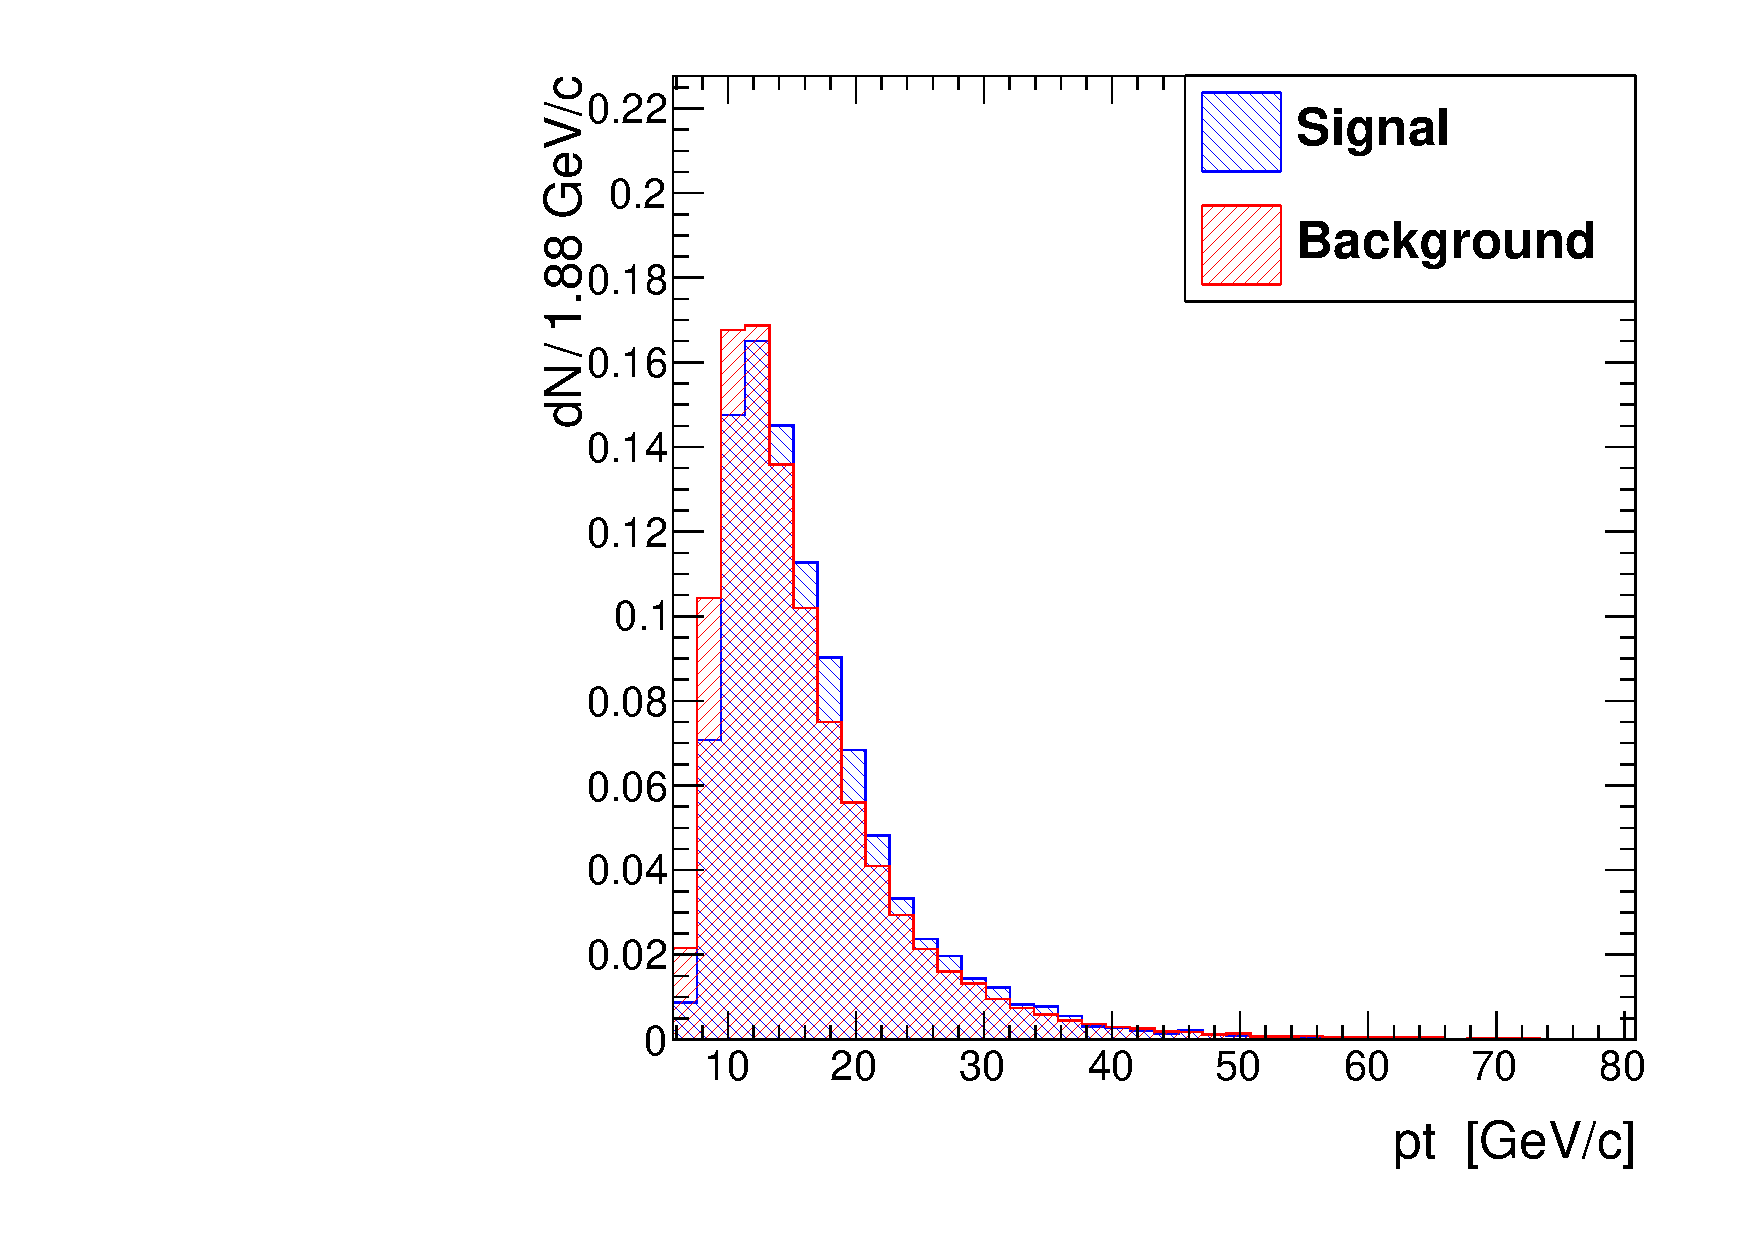
\includegraphics[width=0.3\textwidth]{Figures/pt_barrel}
  %\label{fig:ptBarrel}
  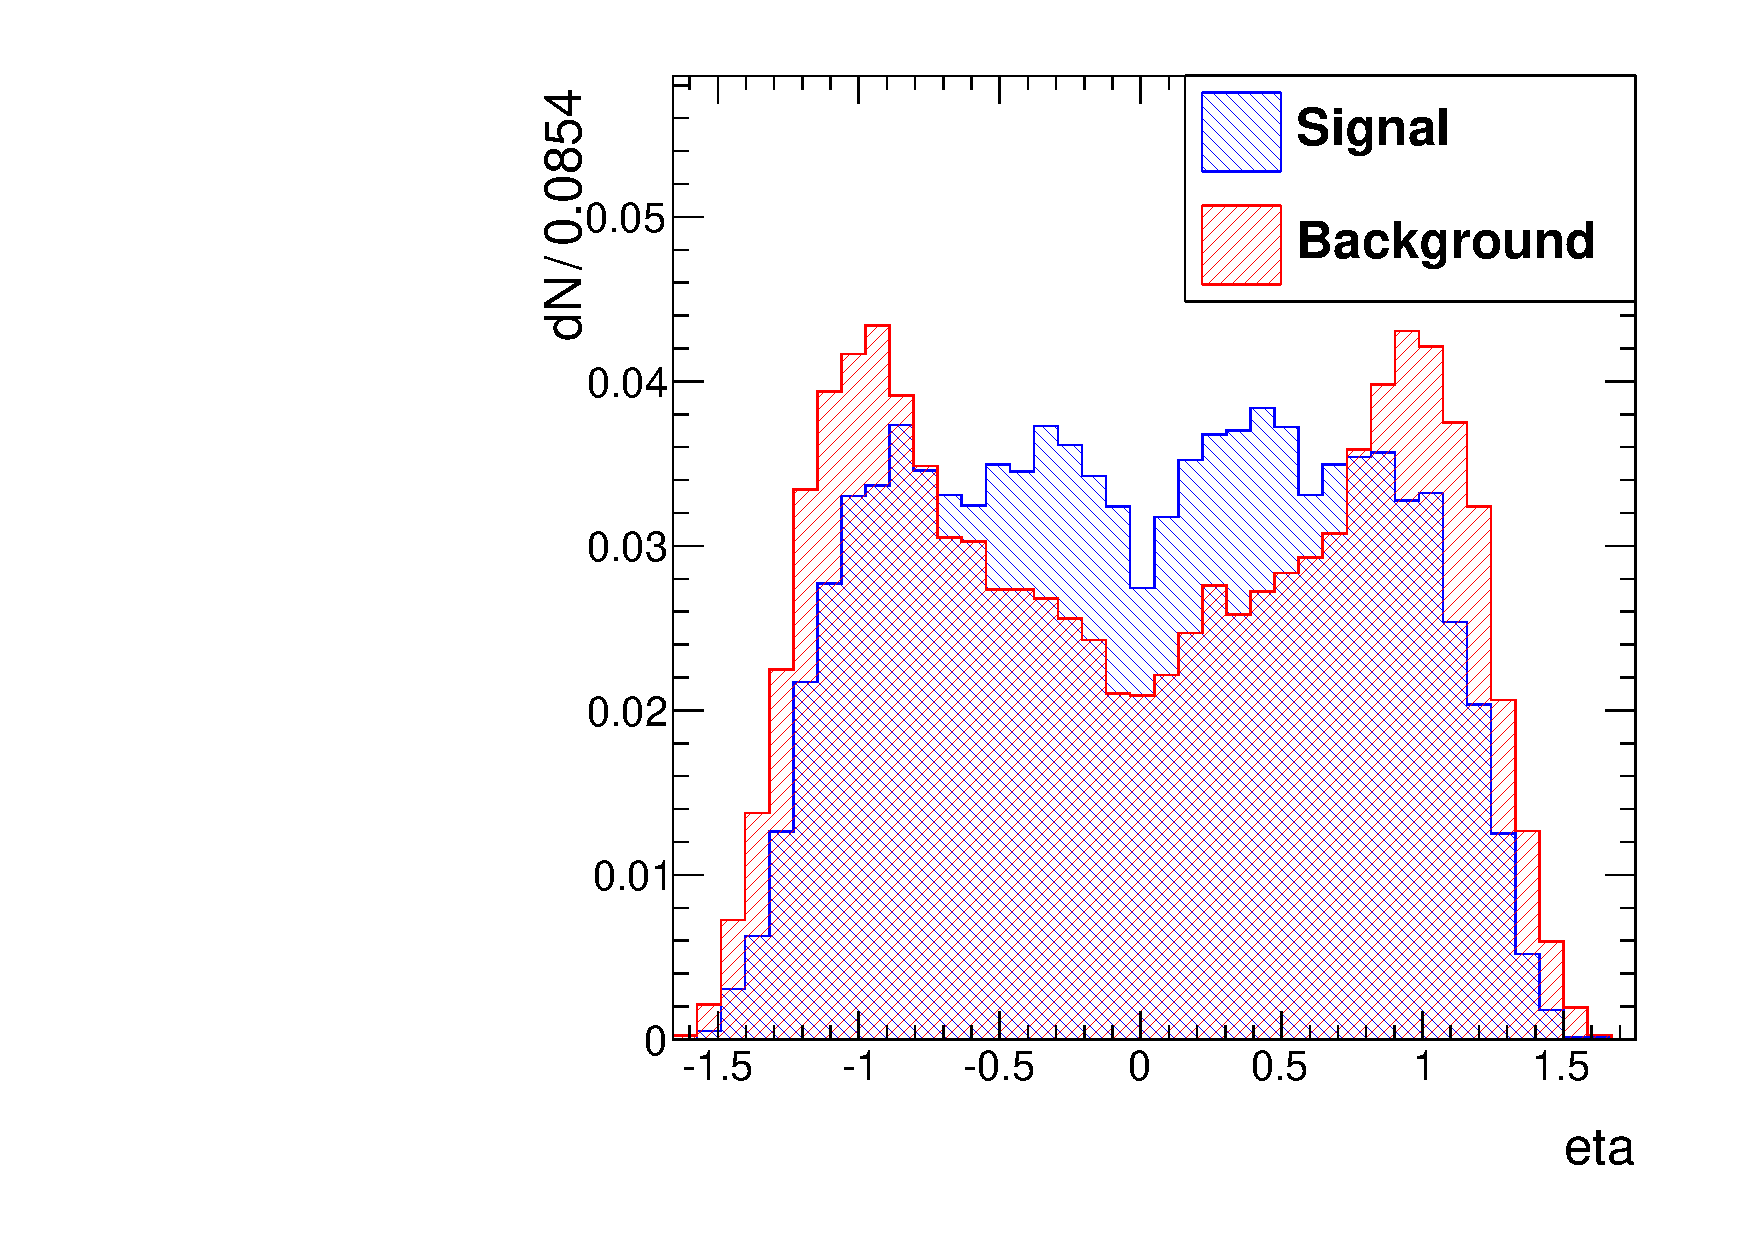
\includegraphics[width=0.3\textwidth]{Figures/eta_barrel}
  %\label{fig:etaBarrel}
  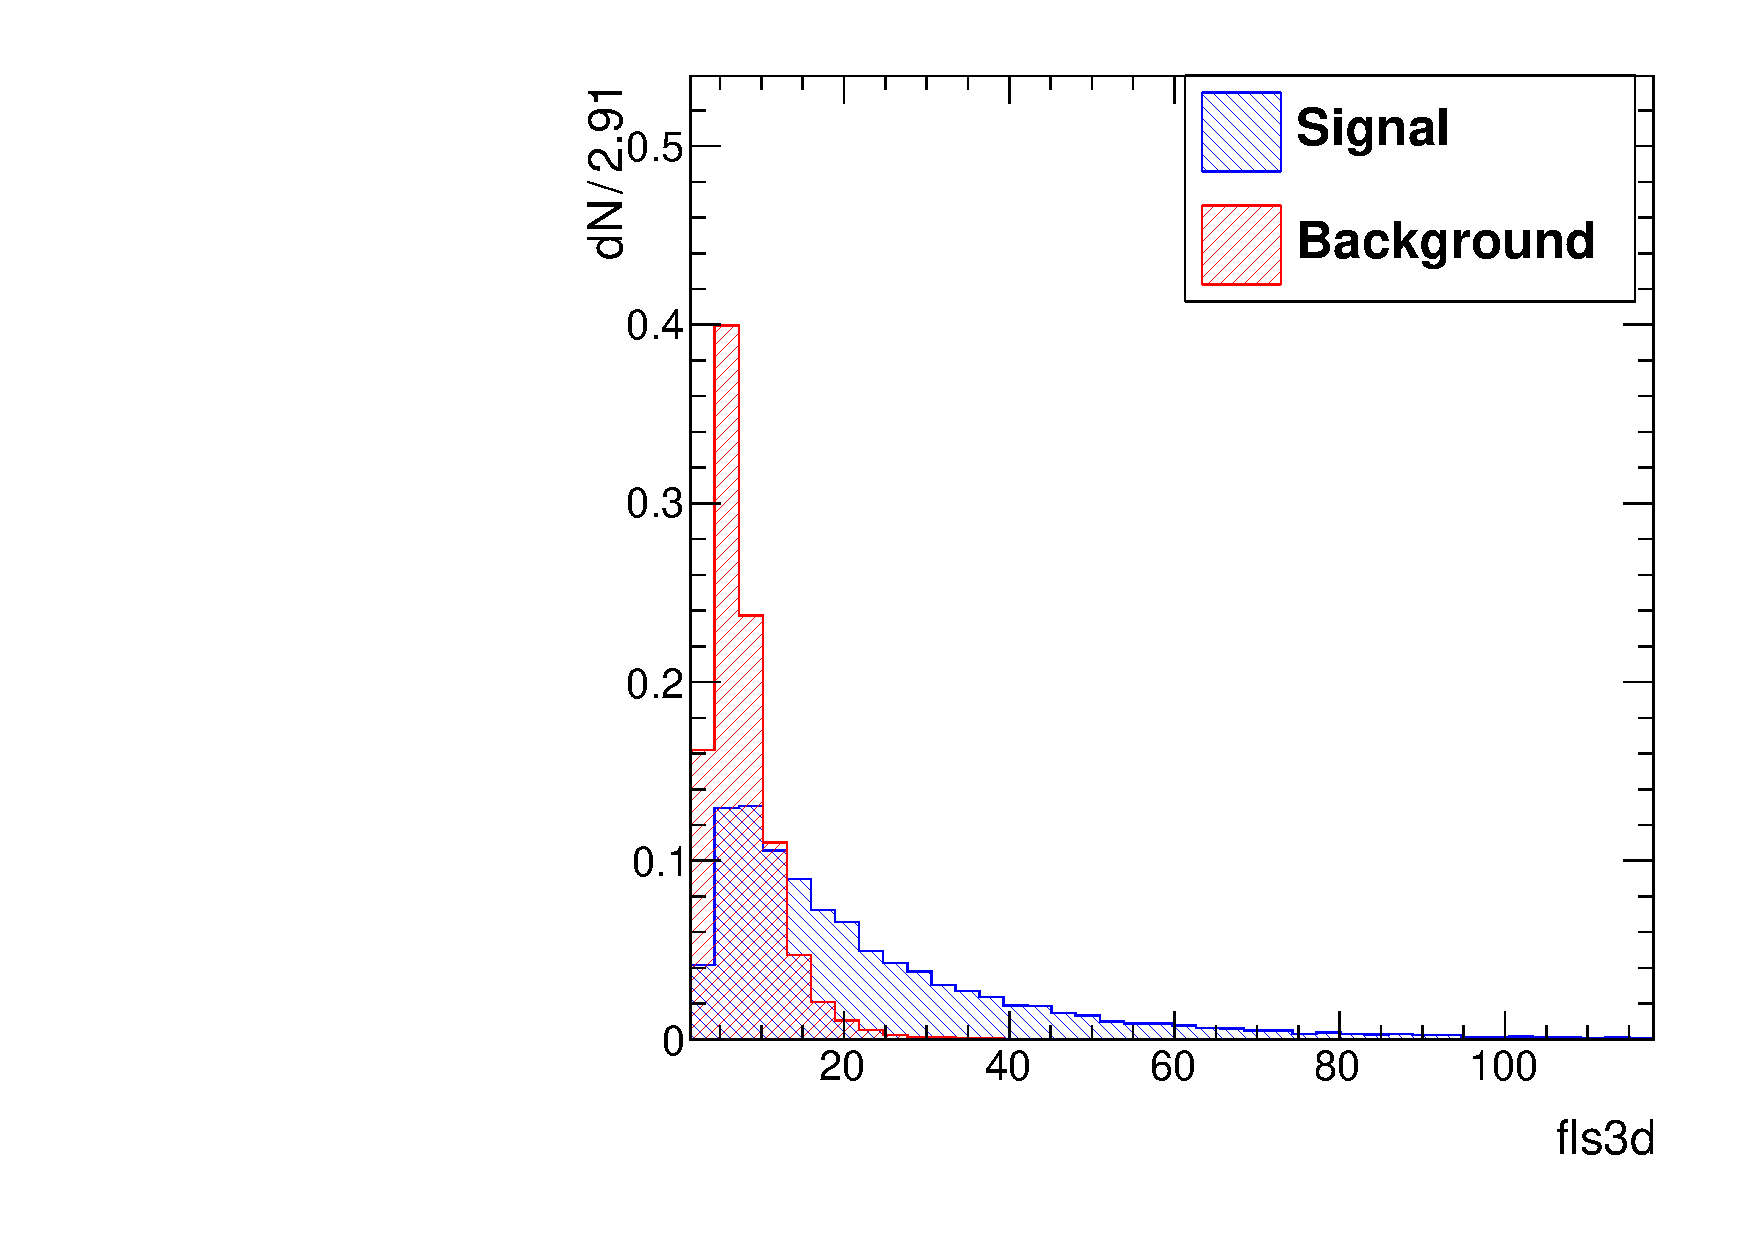
\includegraphics[width=0.3\textwidth]{Figures/fls3d_barrel}
  %\label{fig:fls3dBarrel}
  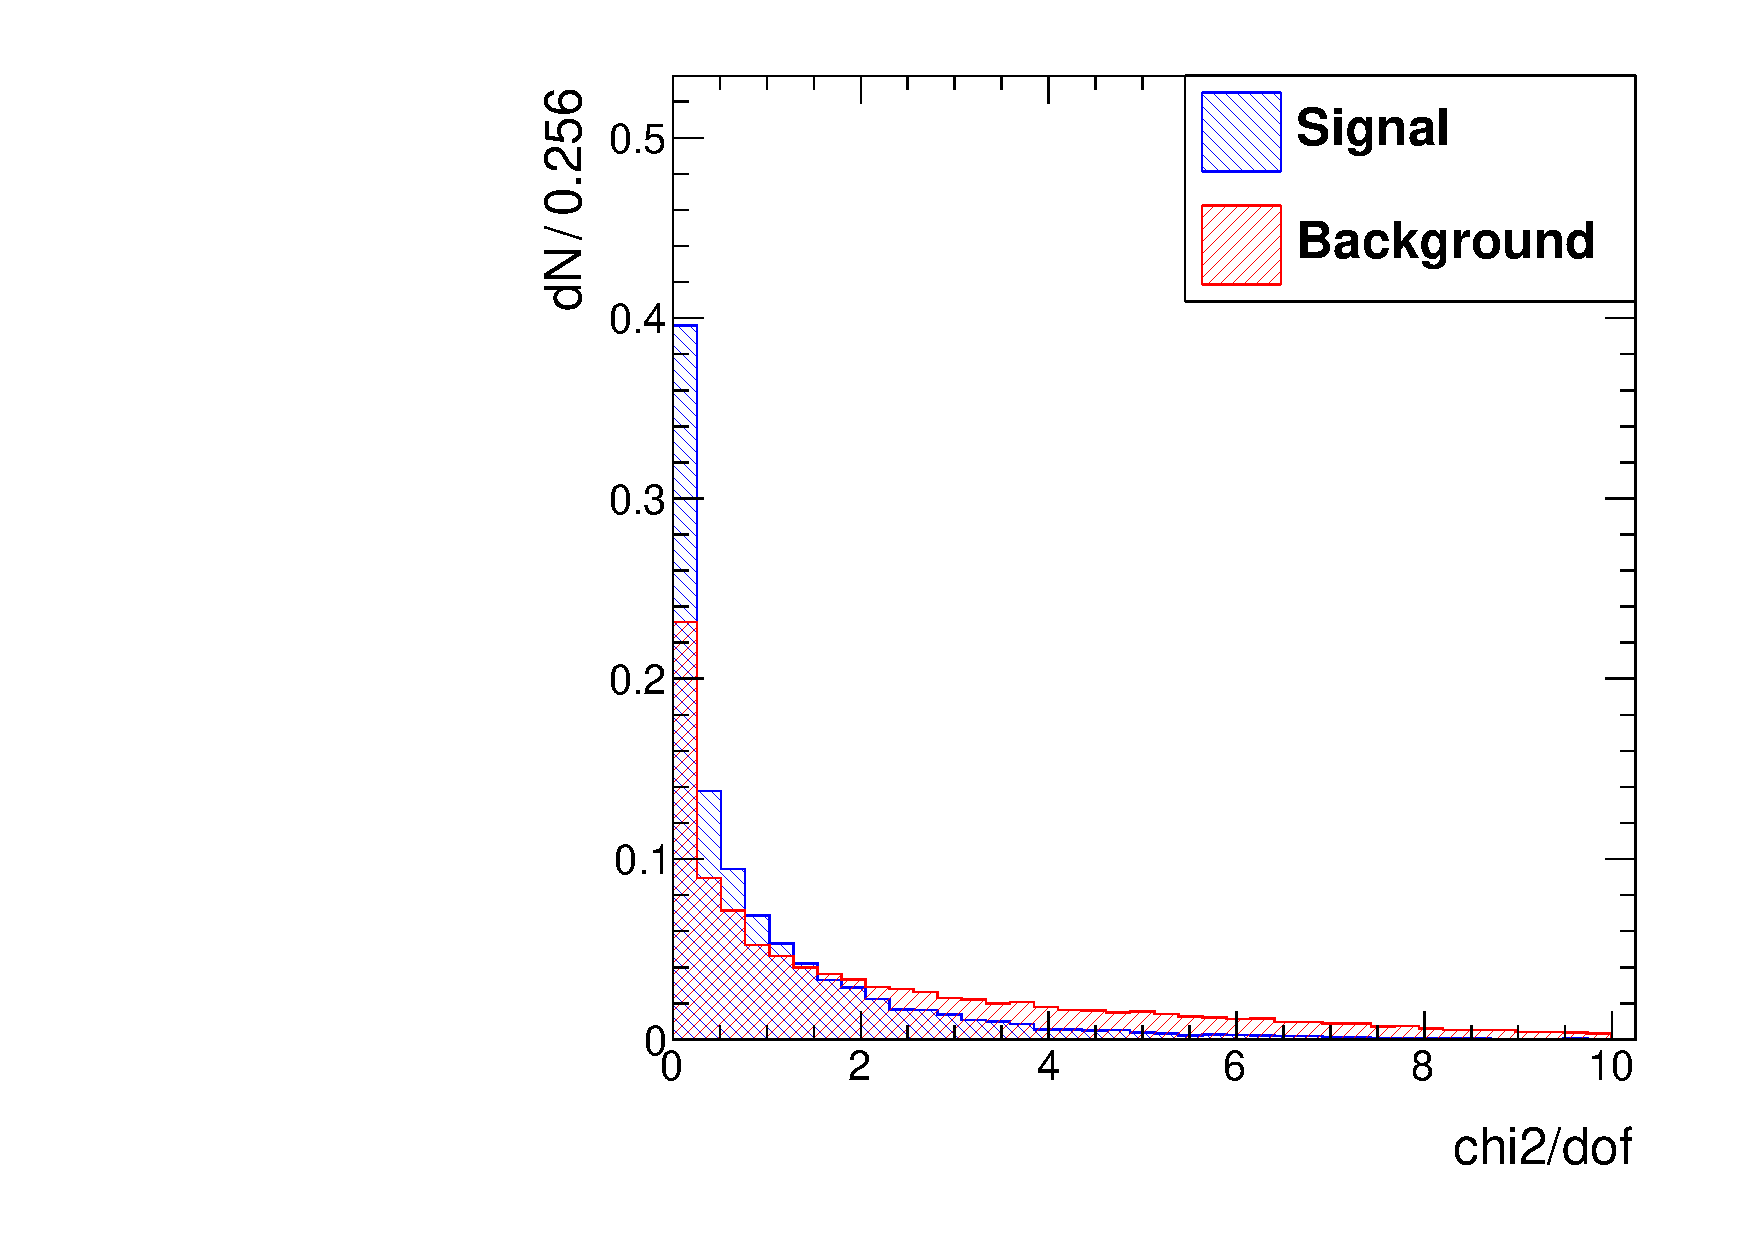
\includegraphics[width=0.3\textwidth]{Figures/chi2dof_barrel}
  %\label{fig:chi2dofBarrel}
  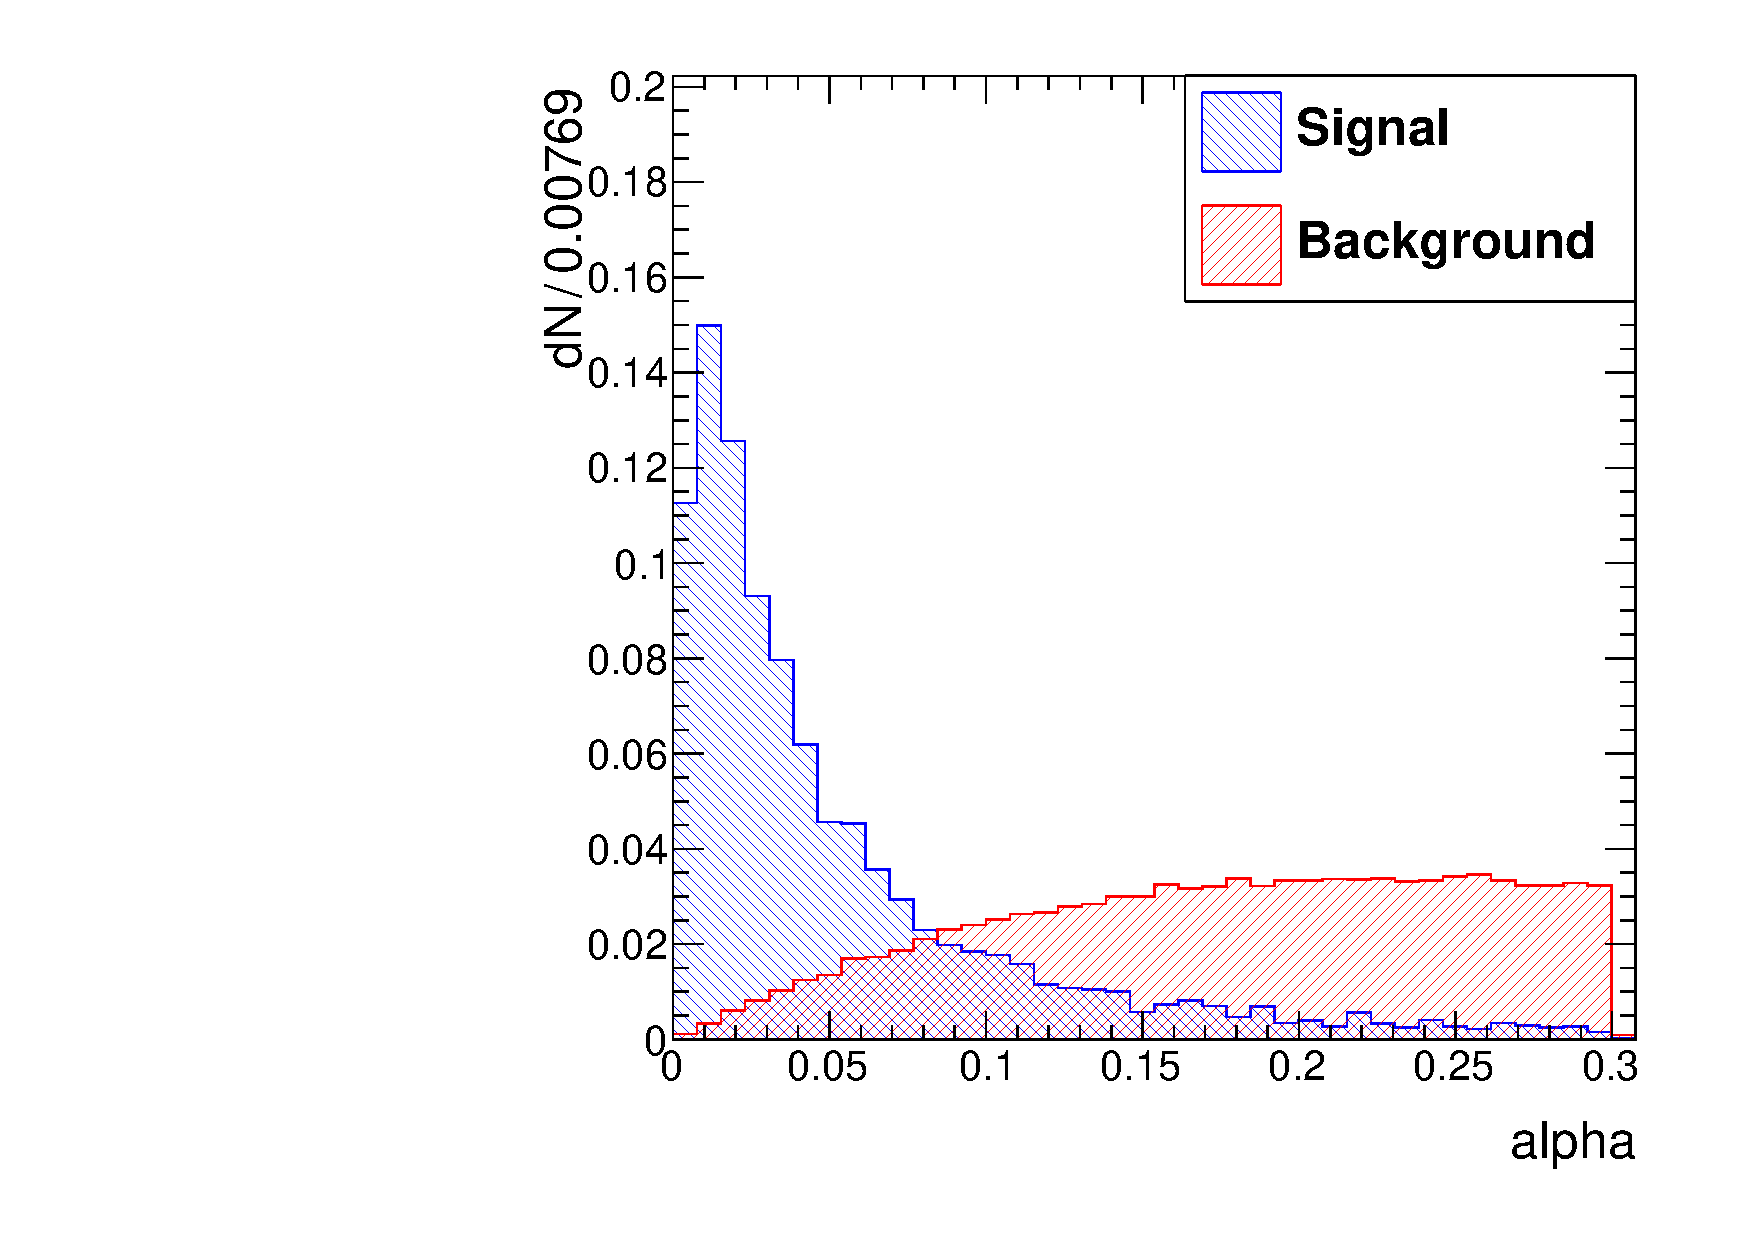
\includegraphics[width=0.3\textwidth]{Figures/alpha_barrel}
  %\label{fig:alphaBarrel}
  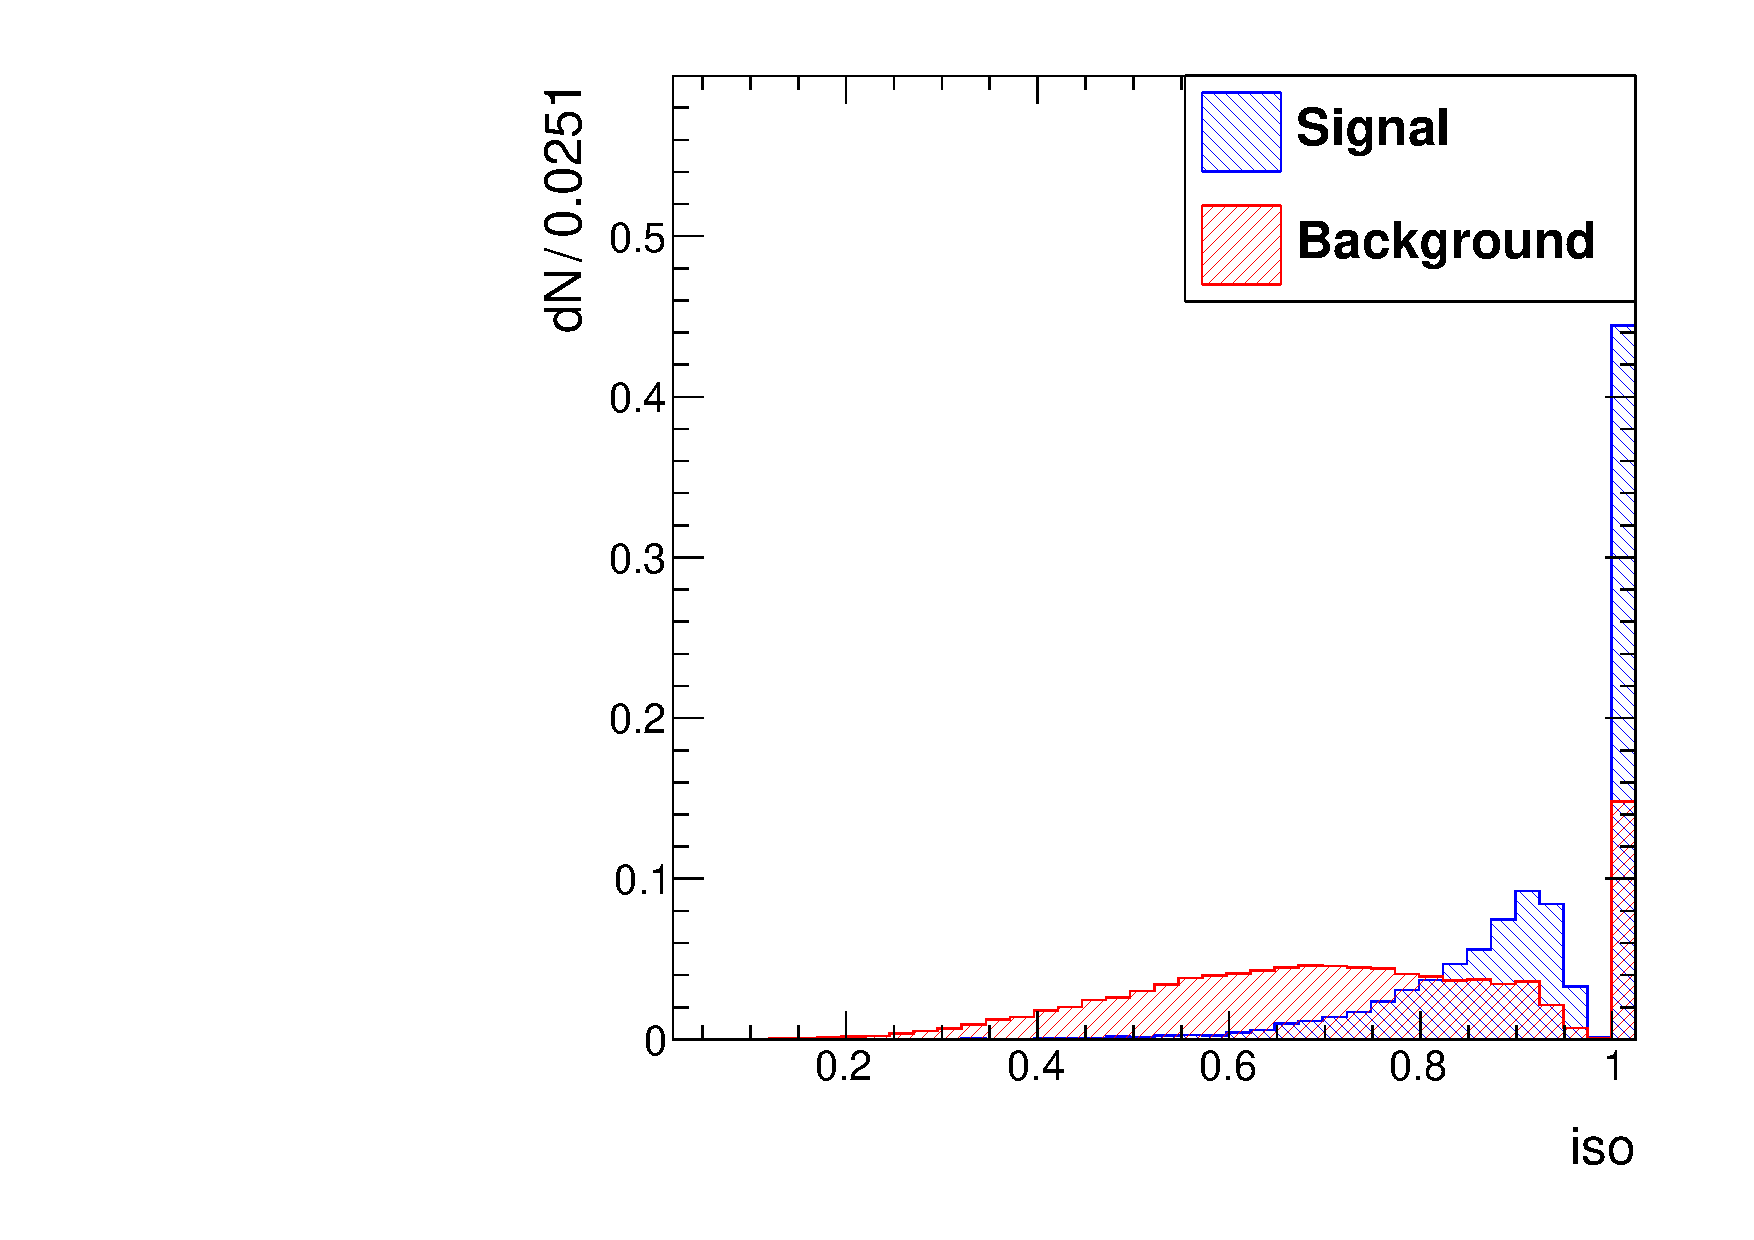
\includegraphics[width=0.3\textwidth]{Figures/iso_barrel}
  %\label{fig:isoBarrel}
  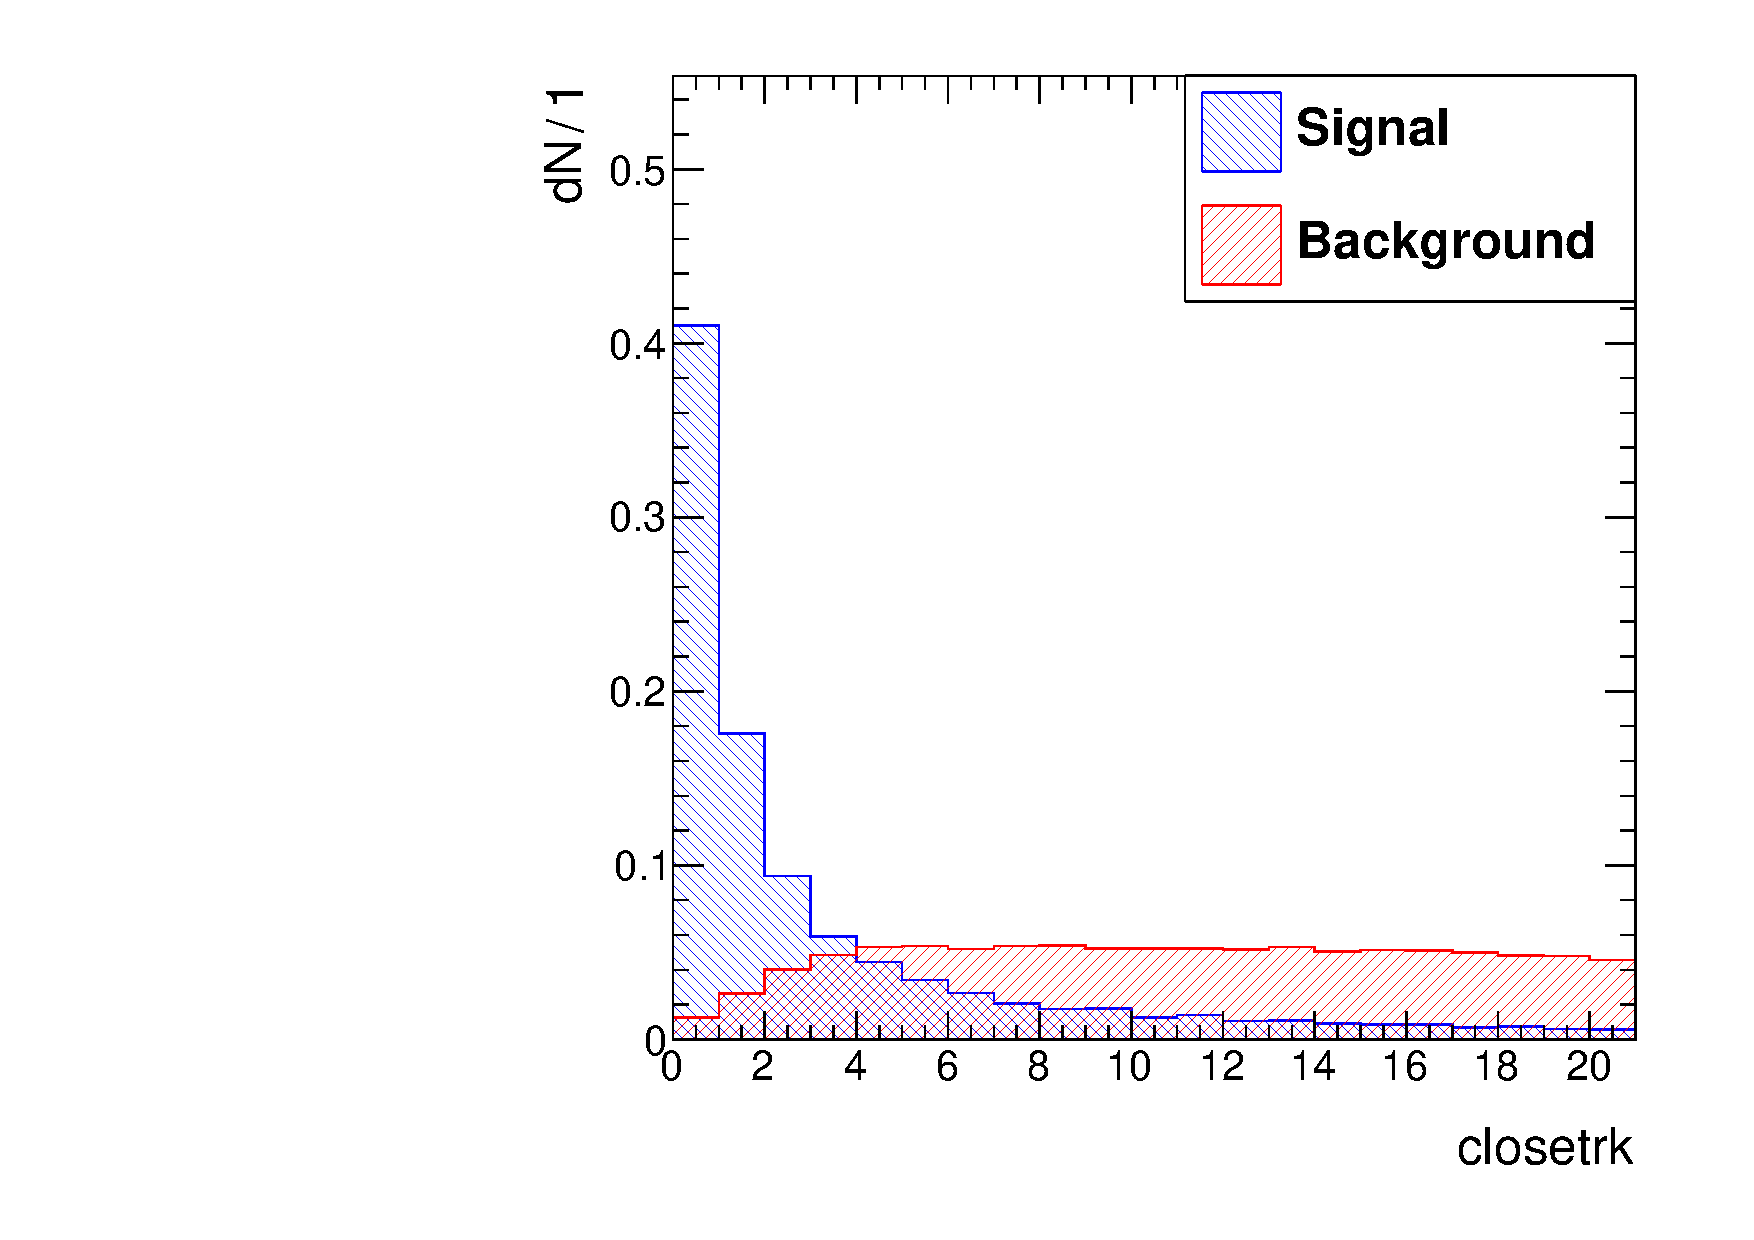
\includegraphics[width=0.3\textwidth]{Figures/closetrk_barrel}
  %\label{fig:closetrkBarrel}
  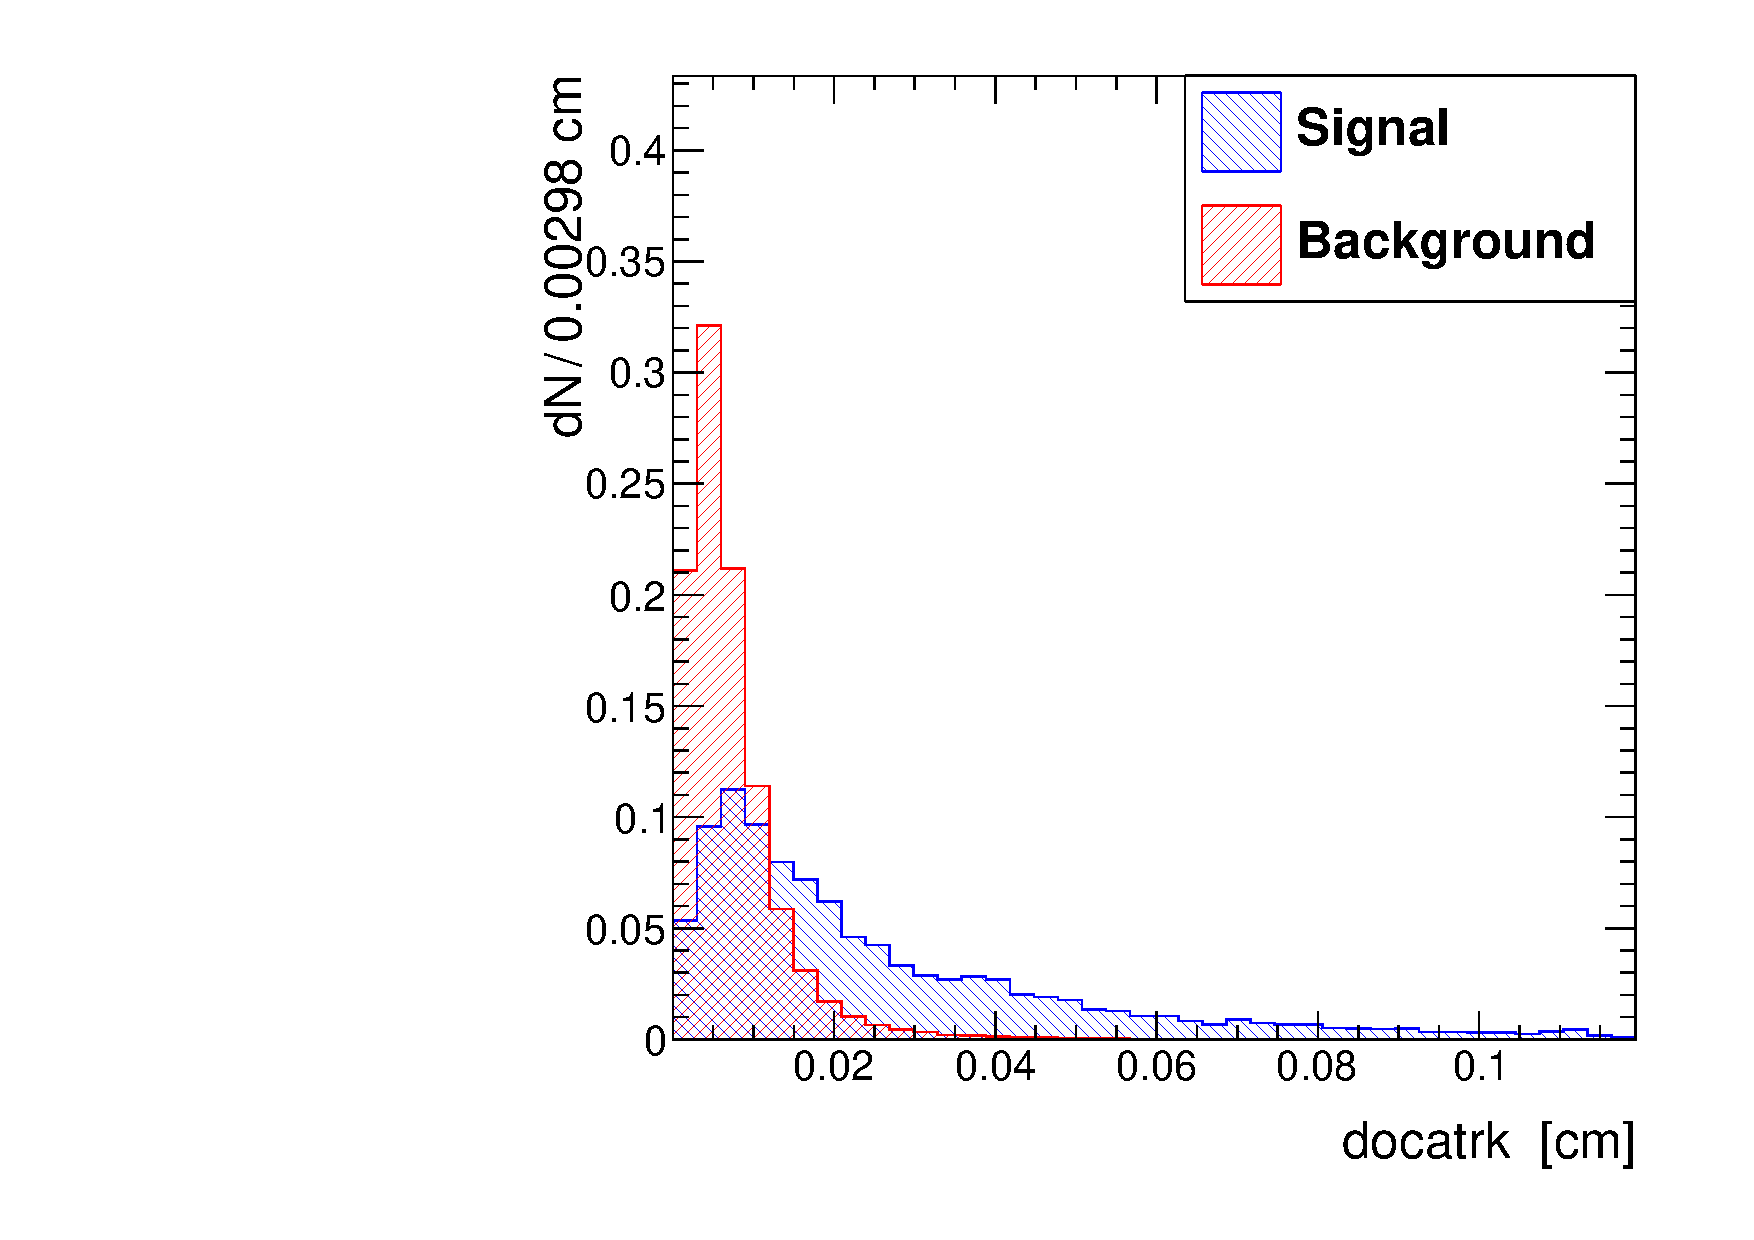
\includegraphics[width=0.3\textwidth]{Figures/docatrk_barrel}
  %\label{fig:docatrkBarrel}
  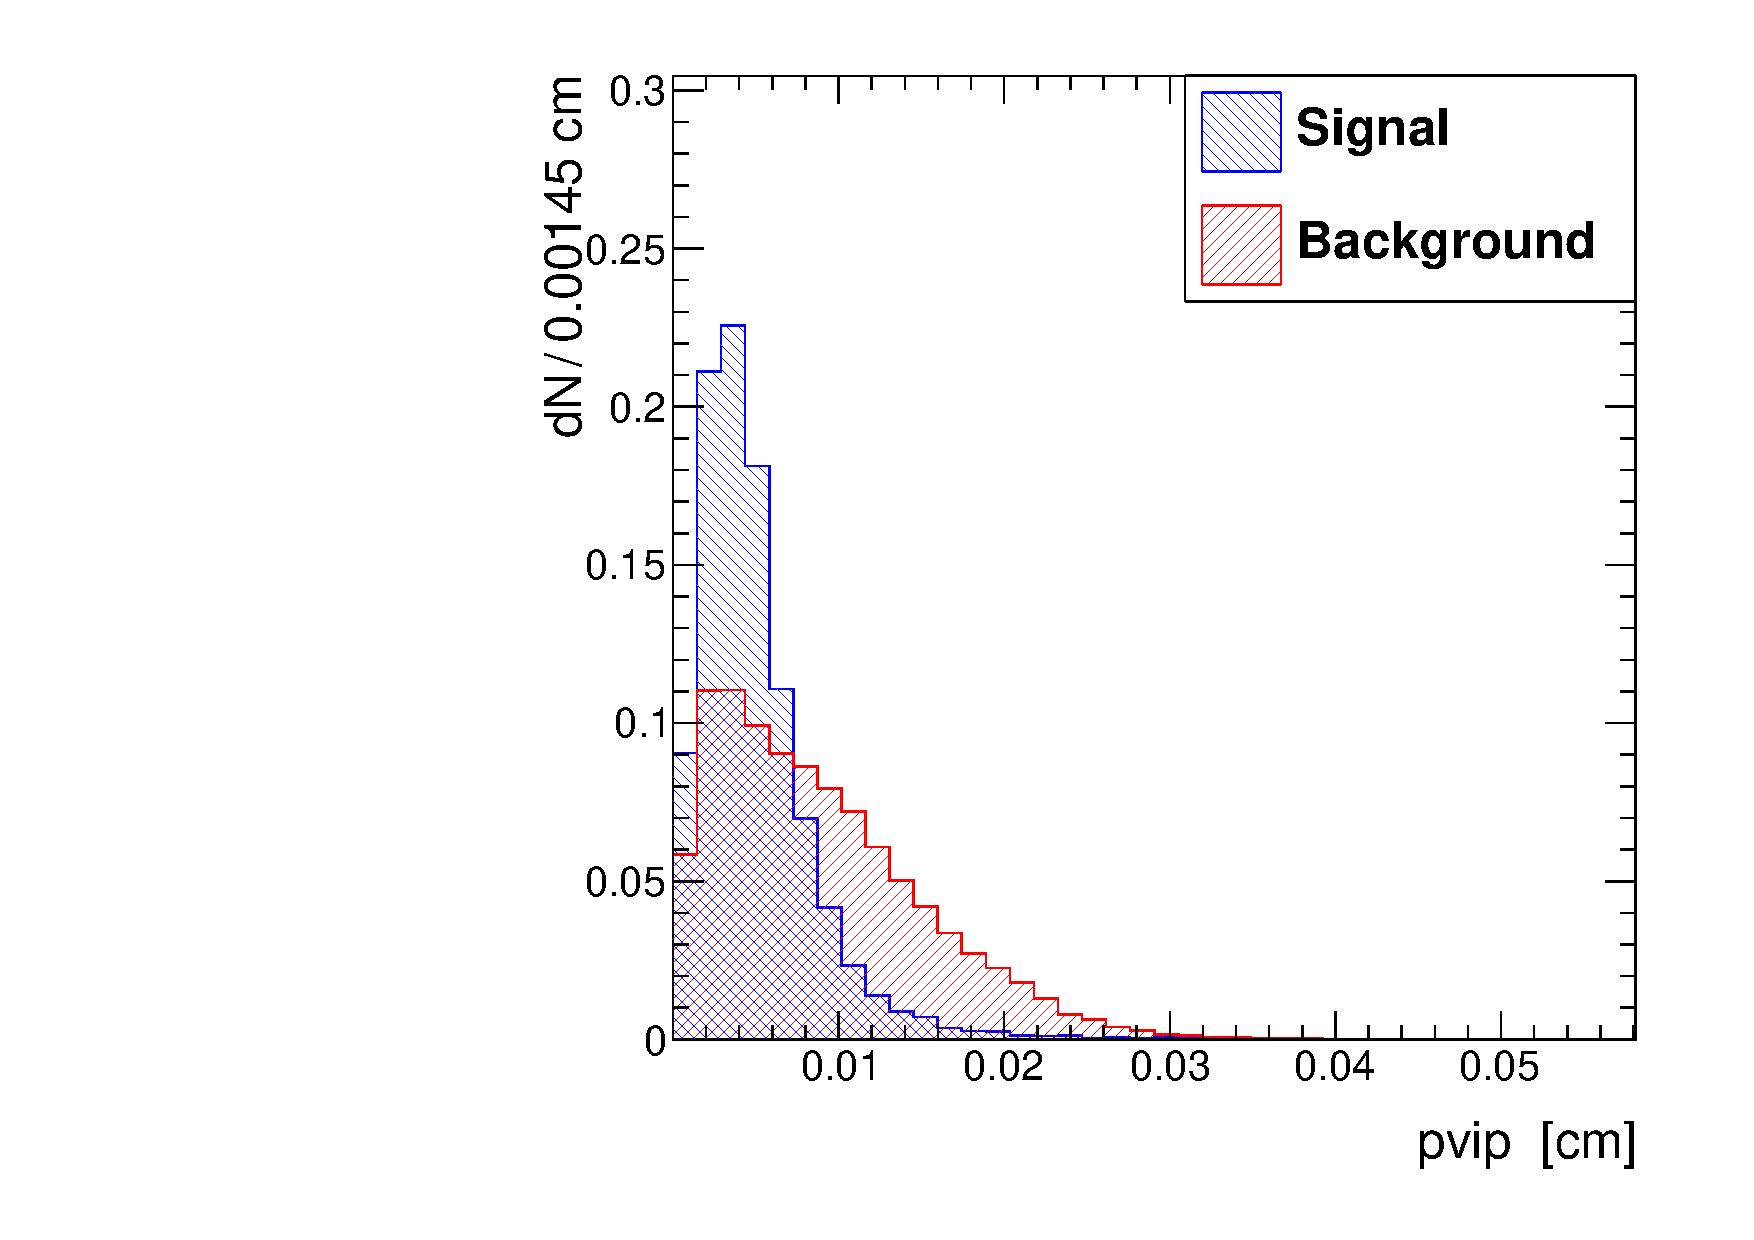
\includegraphics[width=0.3\textwidth]{Figures/pvip_barrel}
  %\label{fig:pvipBarrel}
  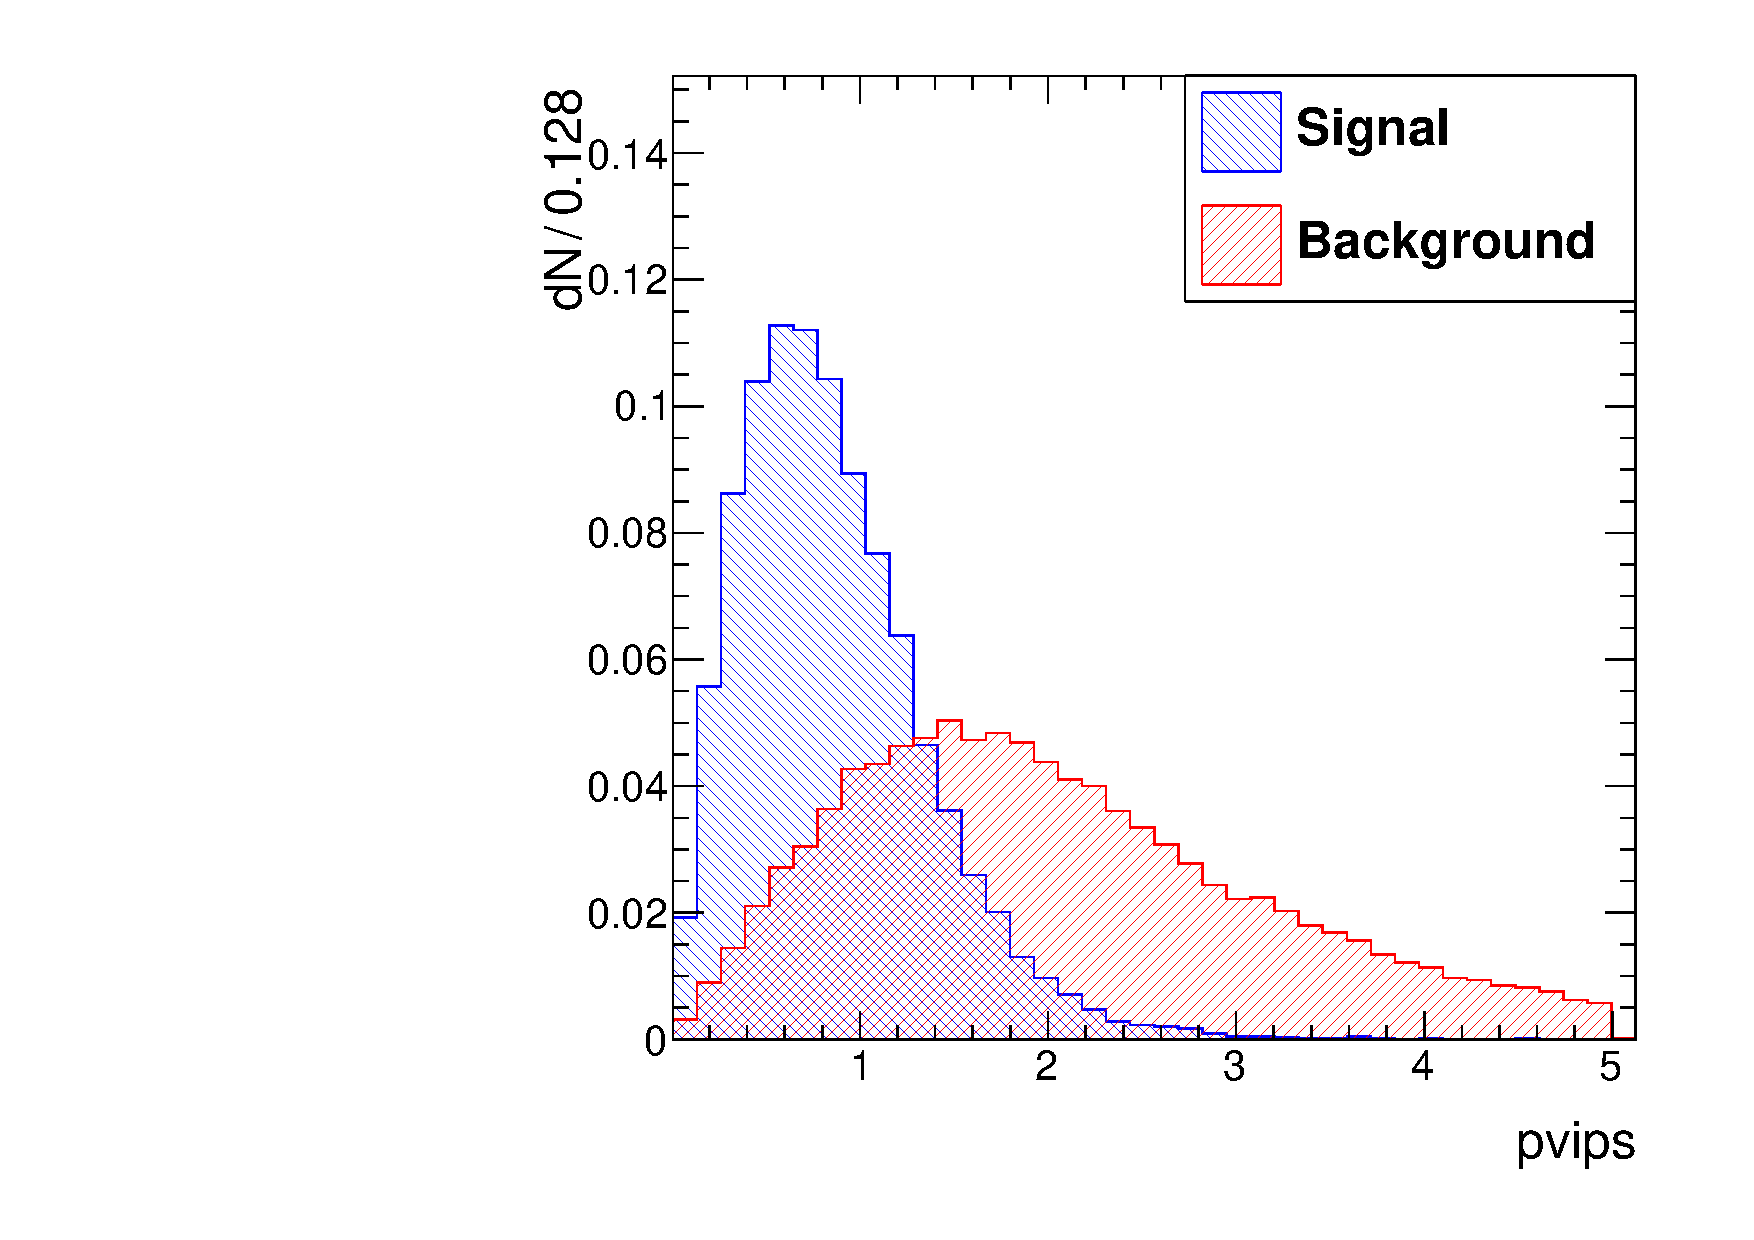
\includegraphics[width=0.3\textwidth]{Figures/pvips_barrel}
  %\label{fig:pvipsBarrel}
  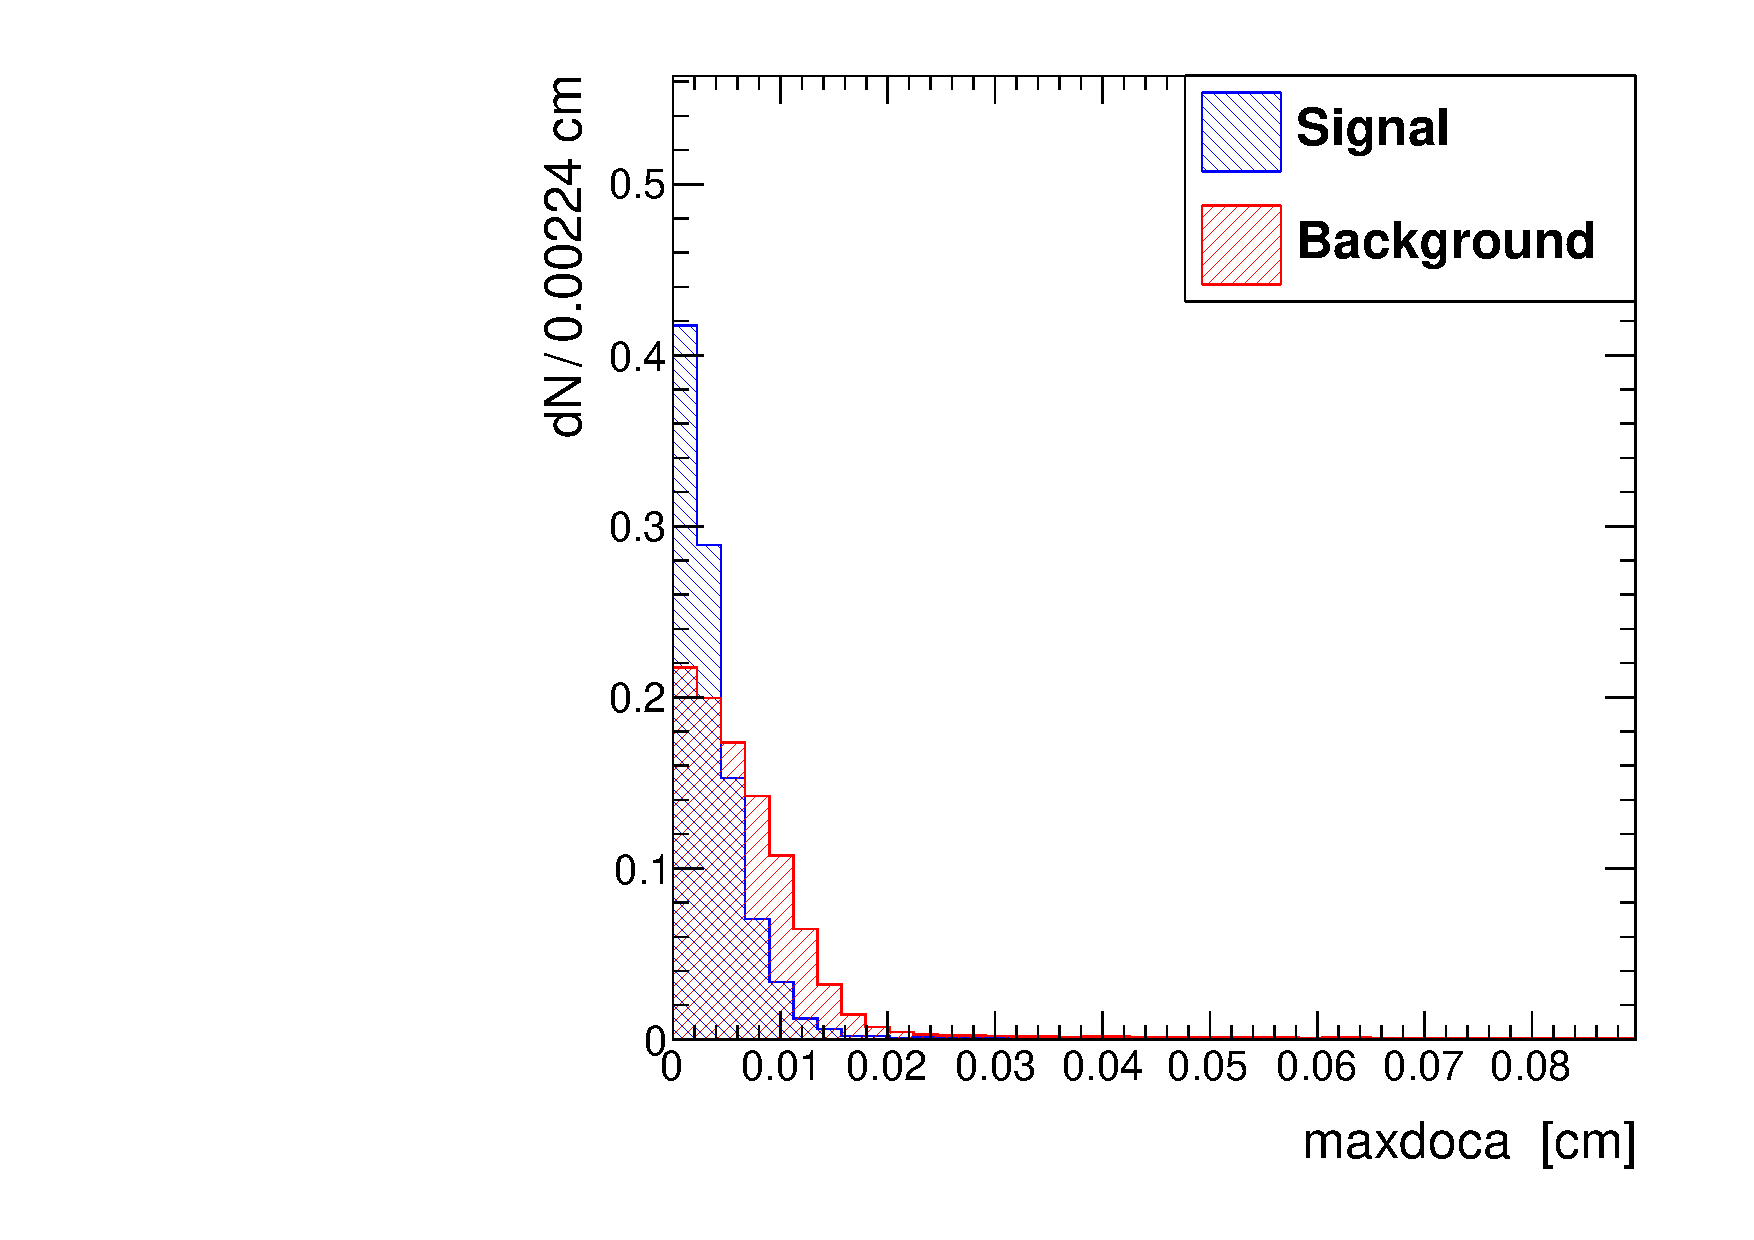
\includegraphics[width=0.3\textwidth]{Figures/maxdoca_barrel}
  %\label{fig:maxdocaBarrel}
  \caption{Standard TMVA plot of the input variables for the barrel BDT for signal (blue) and background (red). The background is extracted from data dimuon sidebands.}
  \label{fig:TMVAPlotsBarrel}
\end{figure}

\begin{figure}
  \centering
  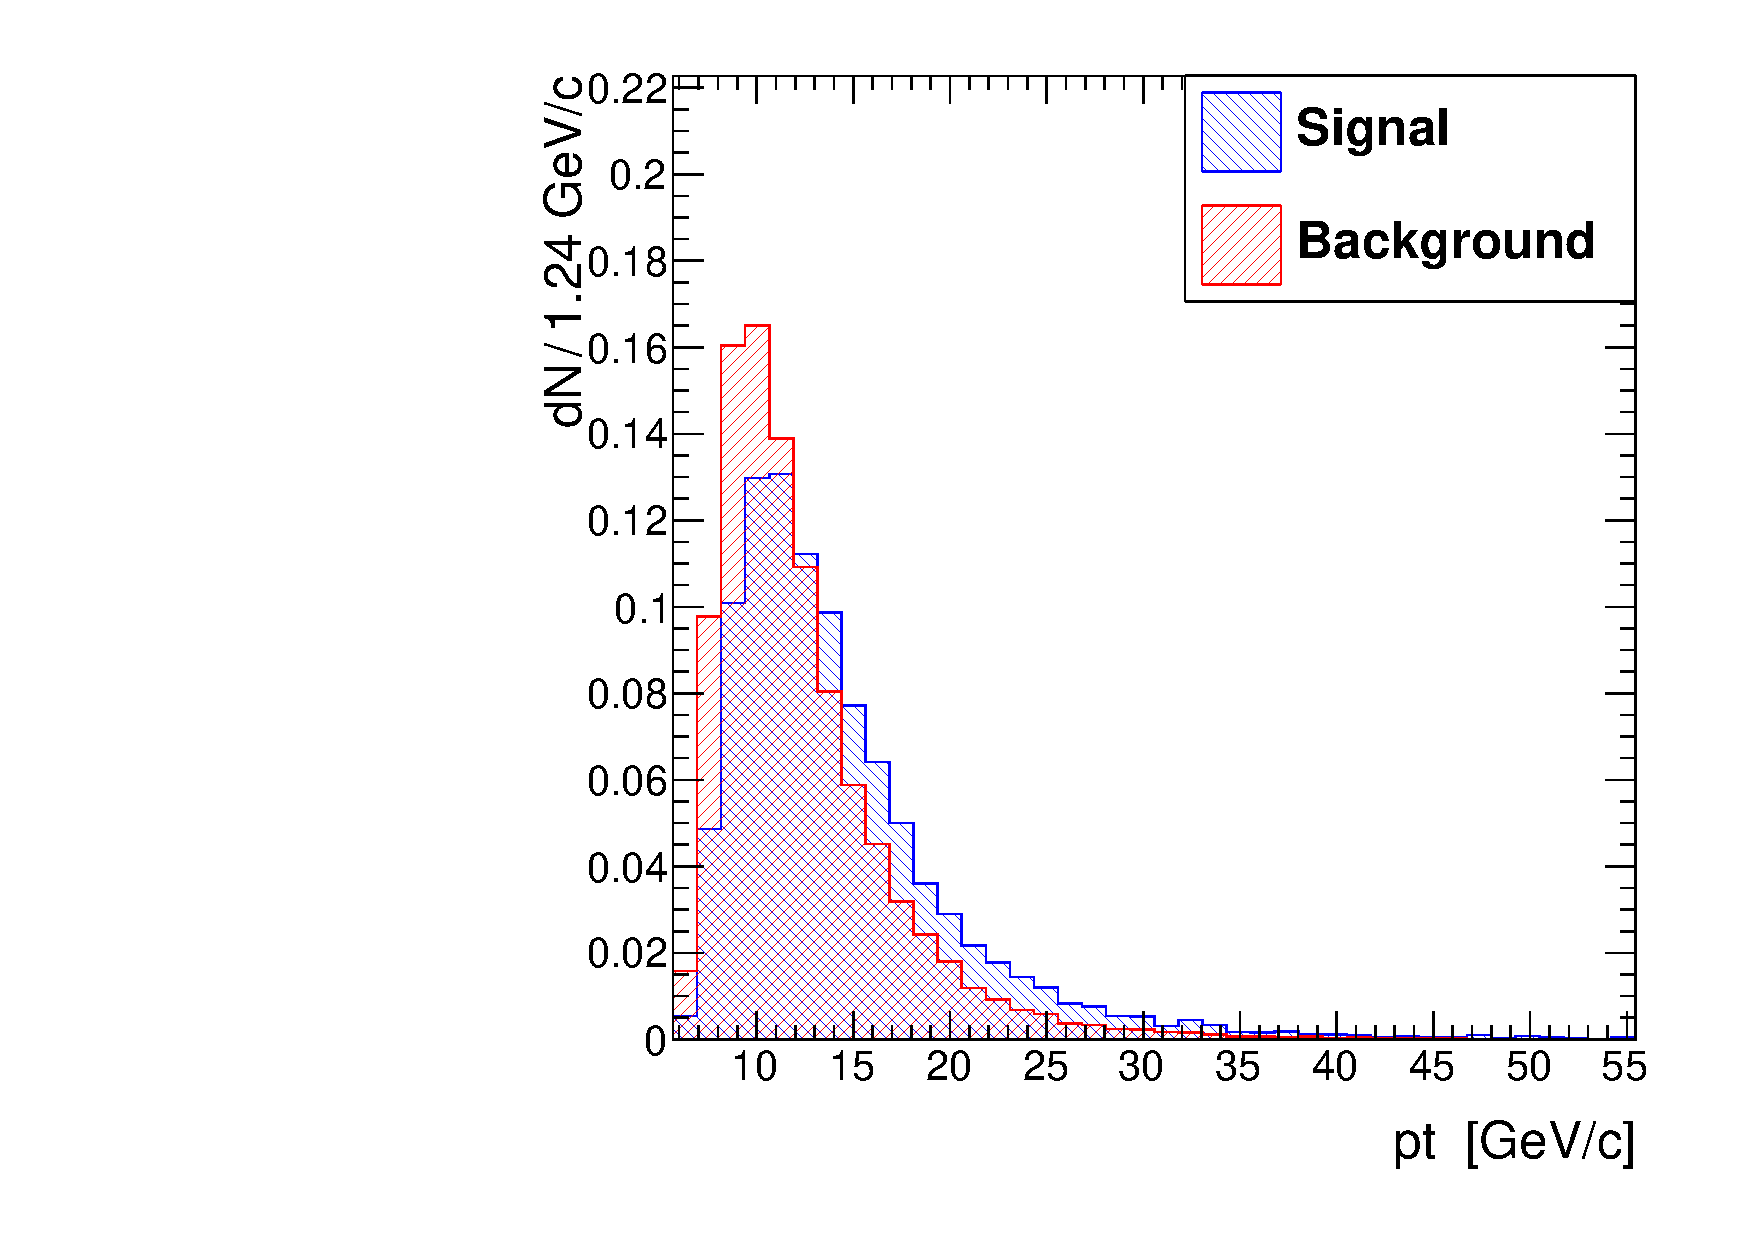
\includegraphics[width=0.3\textwidth]{Figures/pt_endcaps}
  %\label{fig:ptEndcaps}
  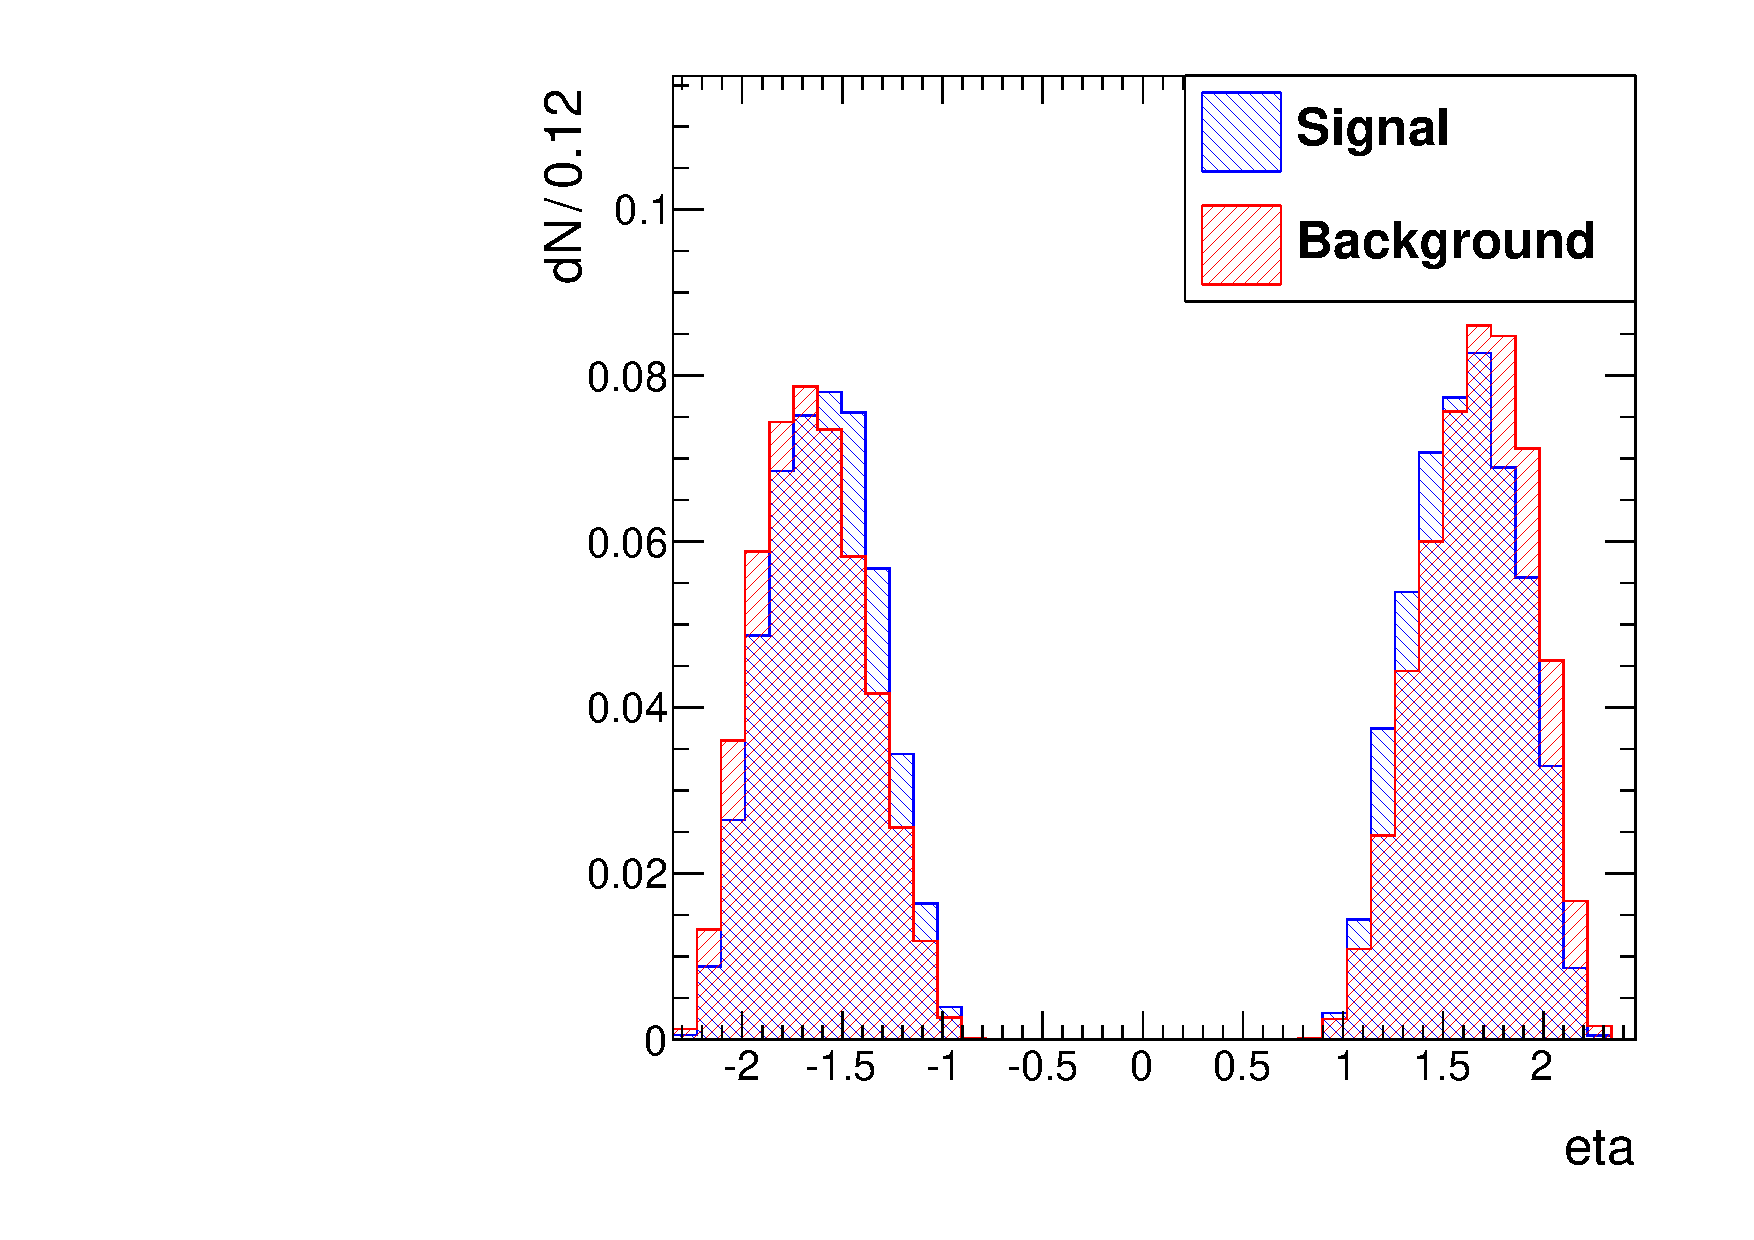
\includegraphics[width=0.3\textwidth]{Figures/eta_endcaps}
  %\label{fig:etaEndcaps}
  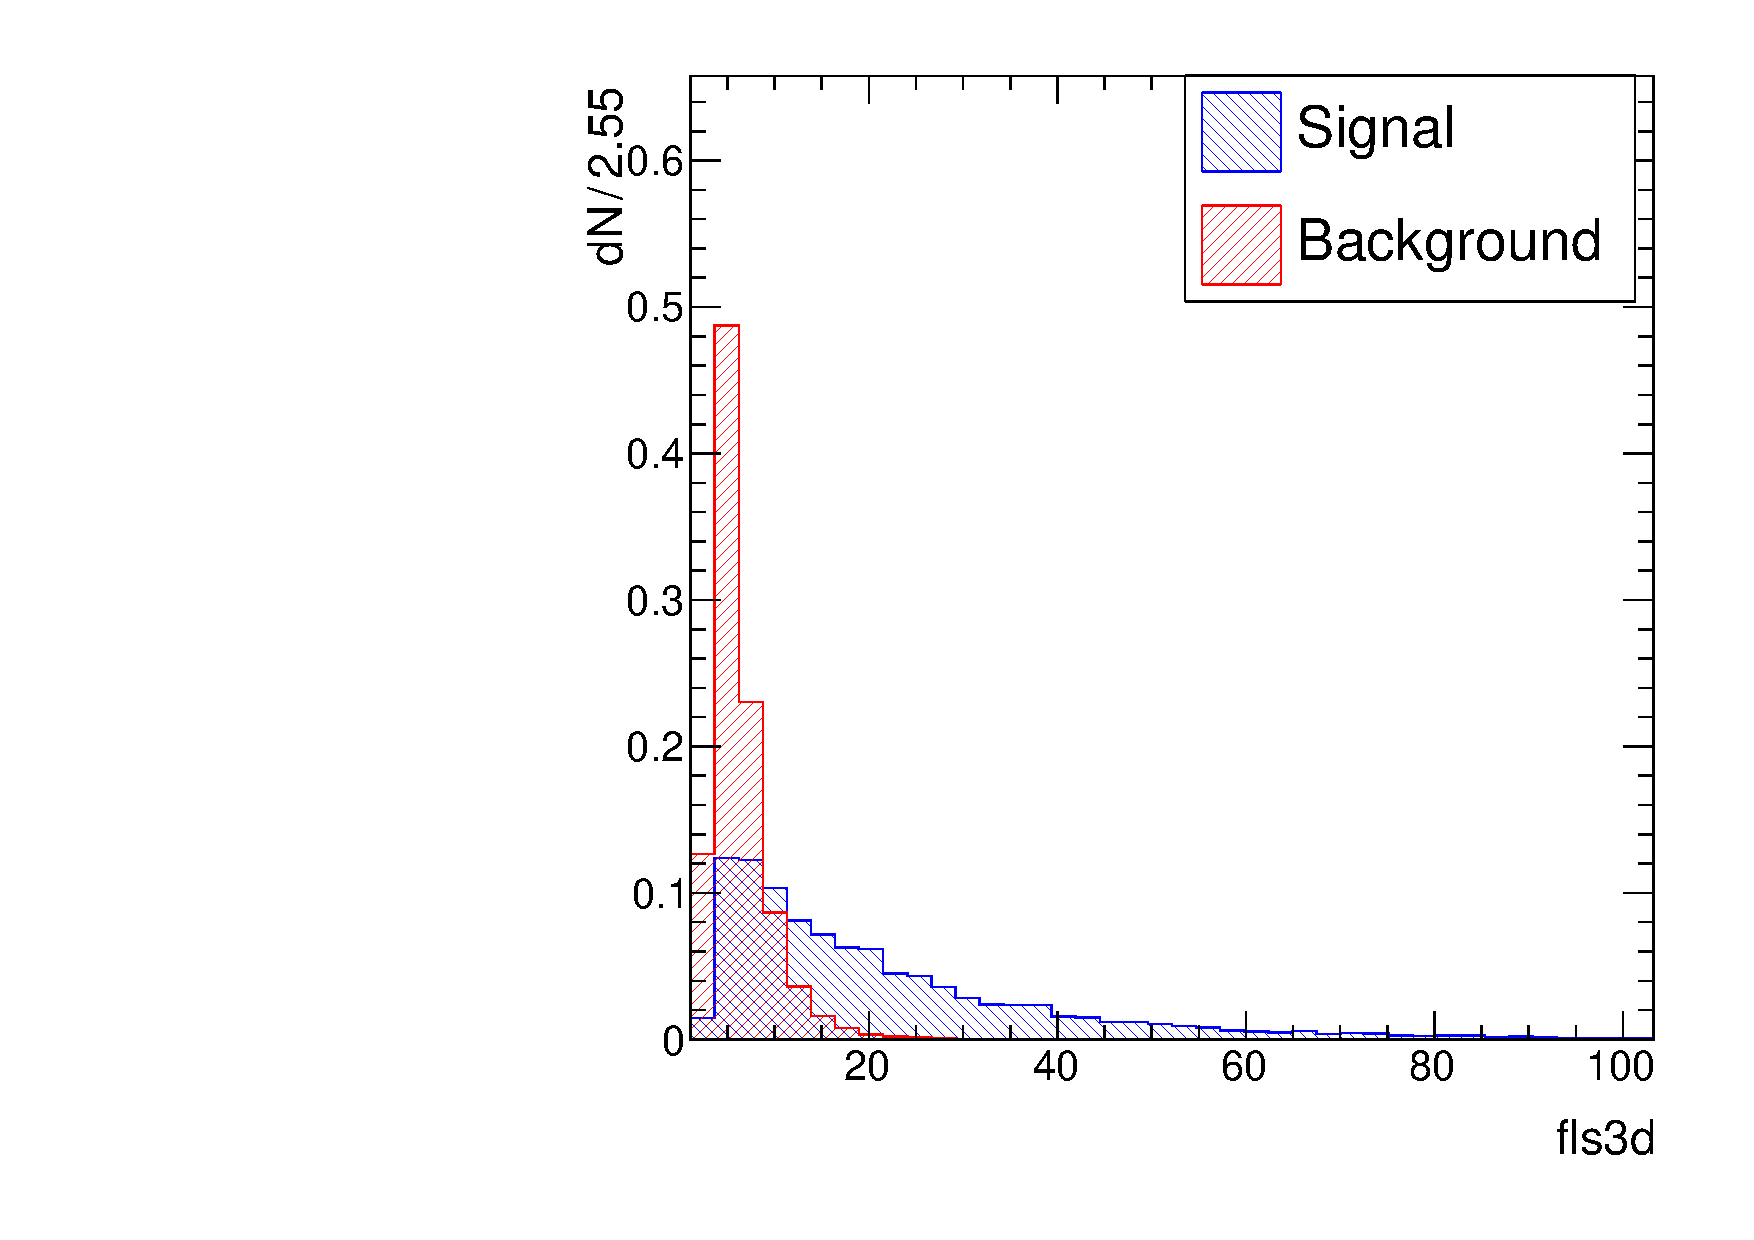
\includegraphics[width=0.3\textwidth]{Figures/fls3d_endcaps}
  %%\label{fig:fls3dEndcaps}
  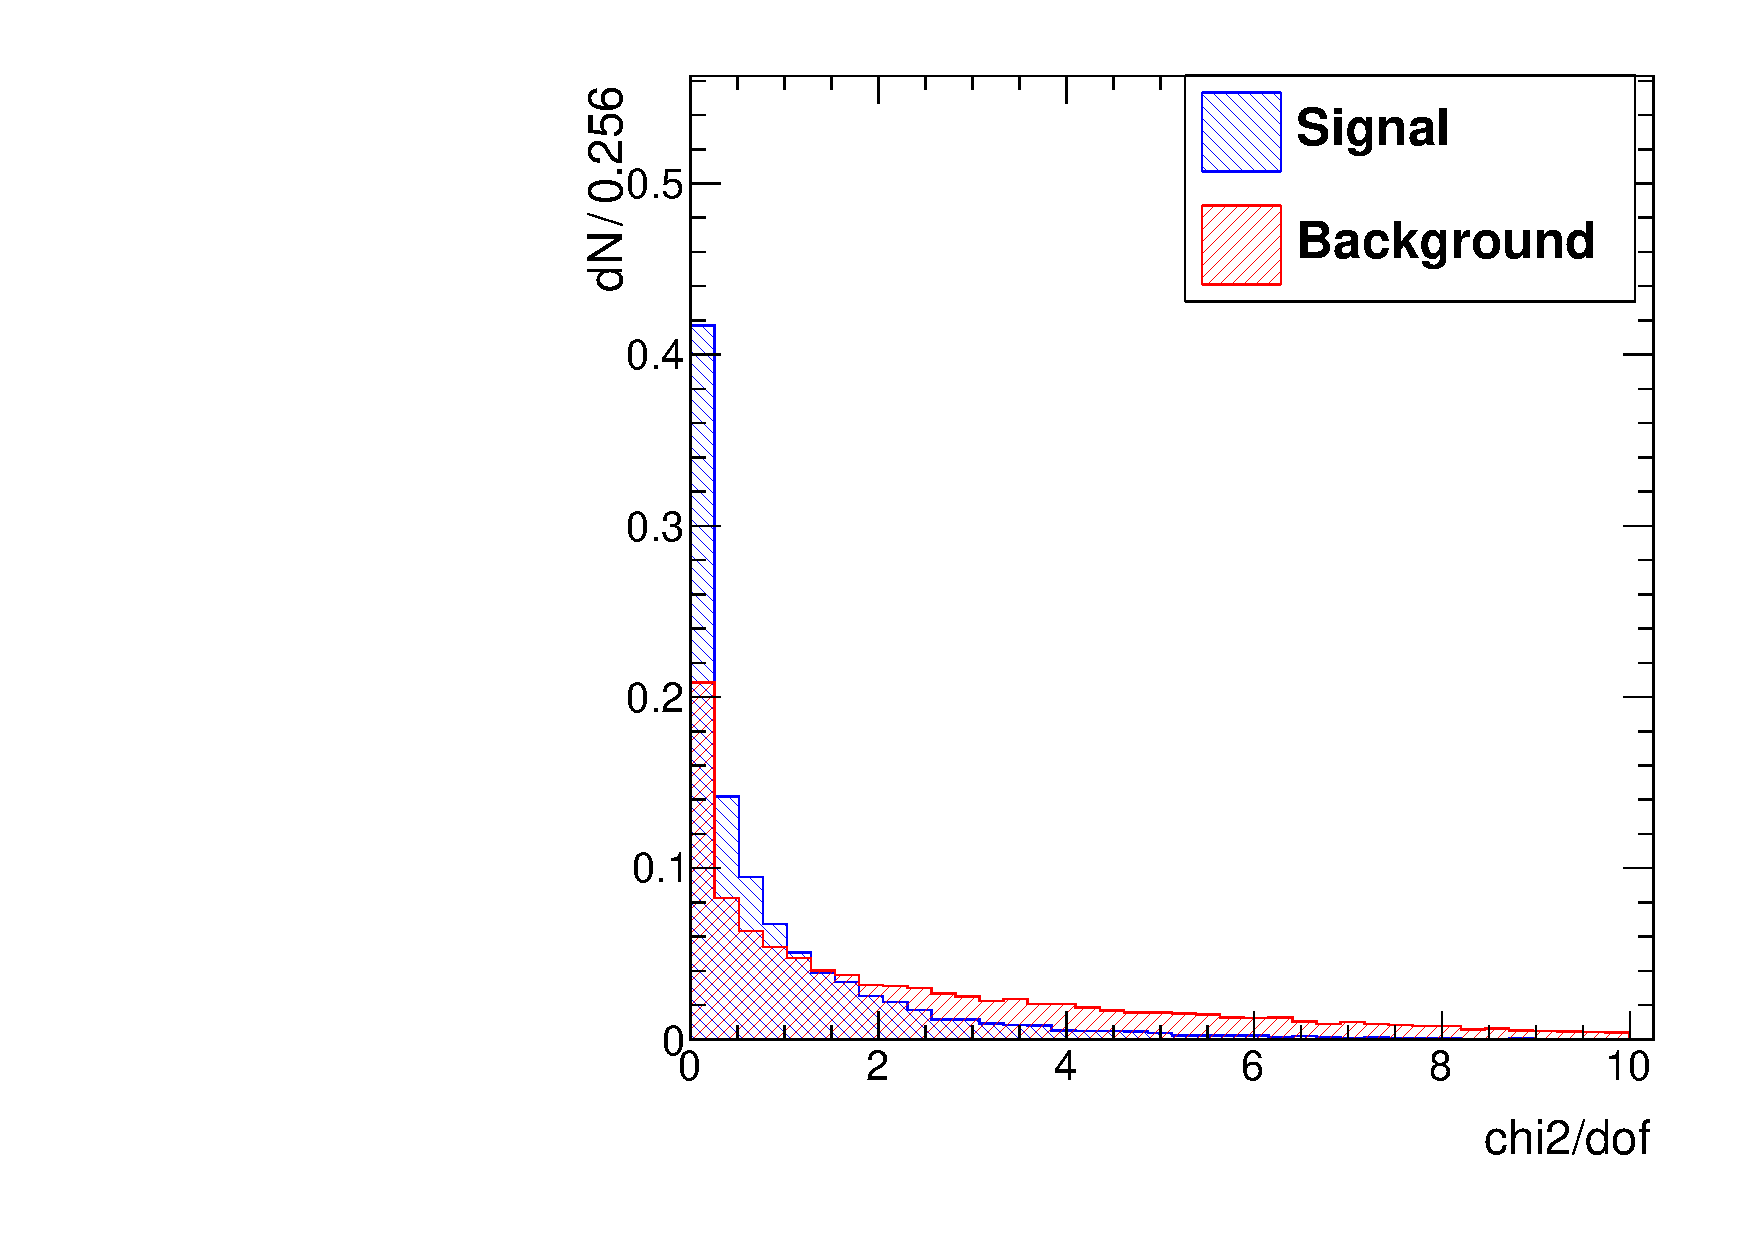
\includegraphics[width=0.3\textwidth]{Figures/chi2dof_endcaps}
  %\label{fig:chi2dofEndcaps}
  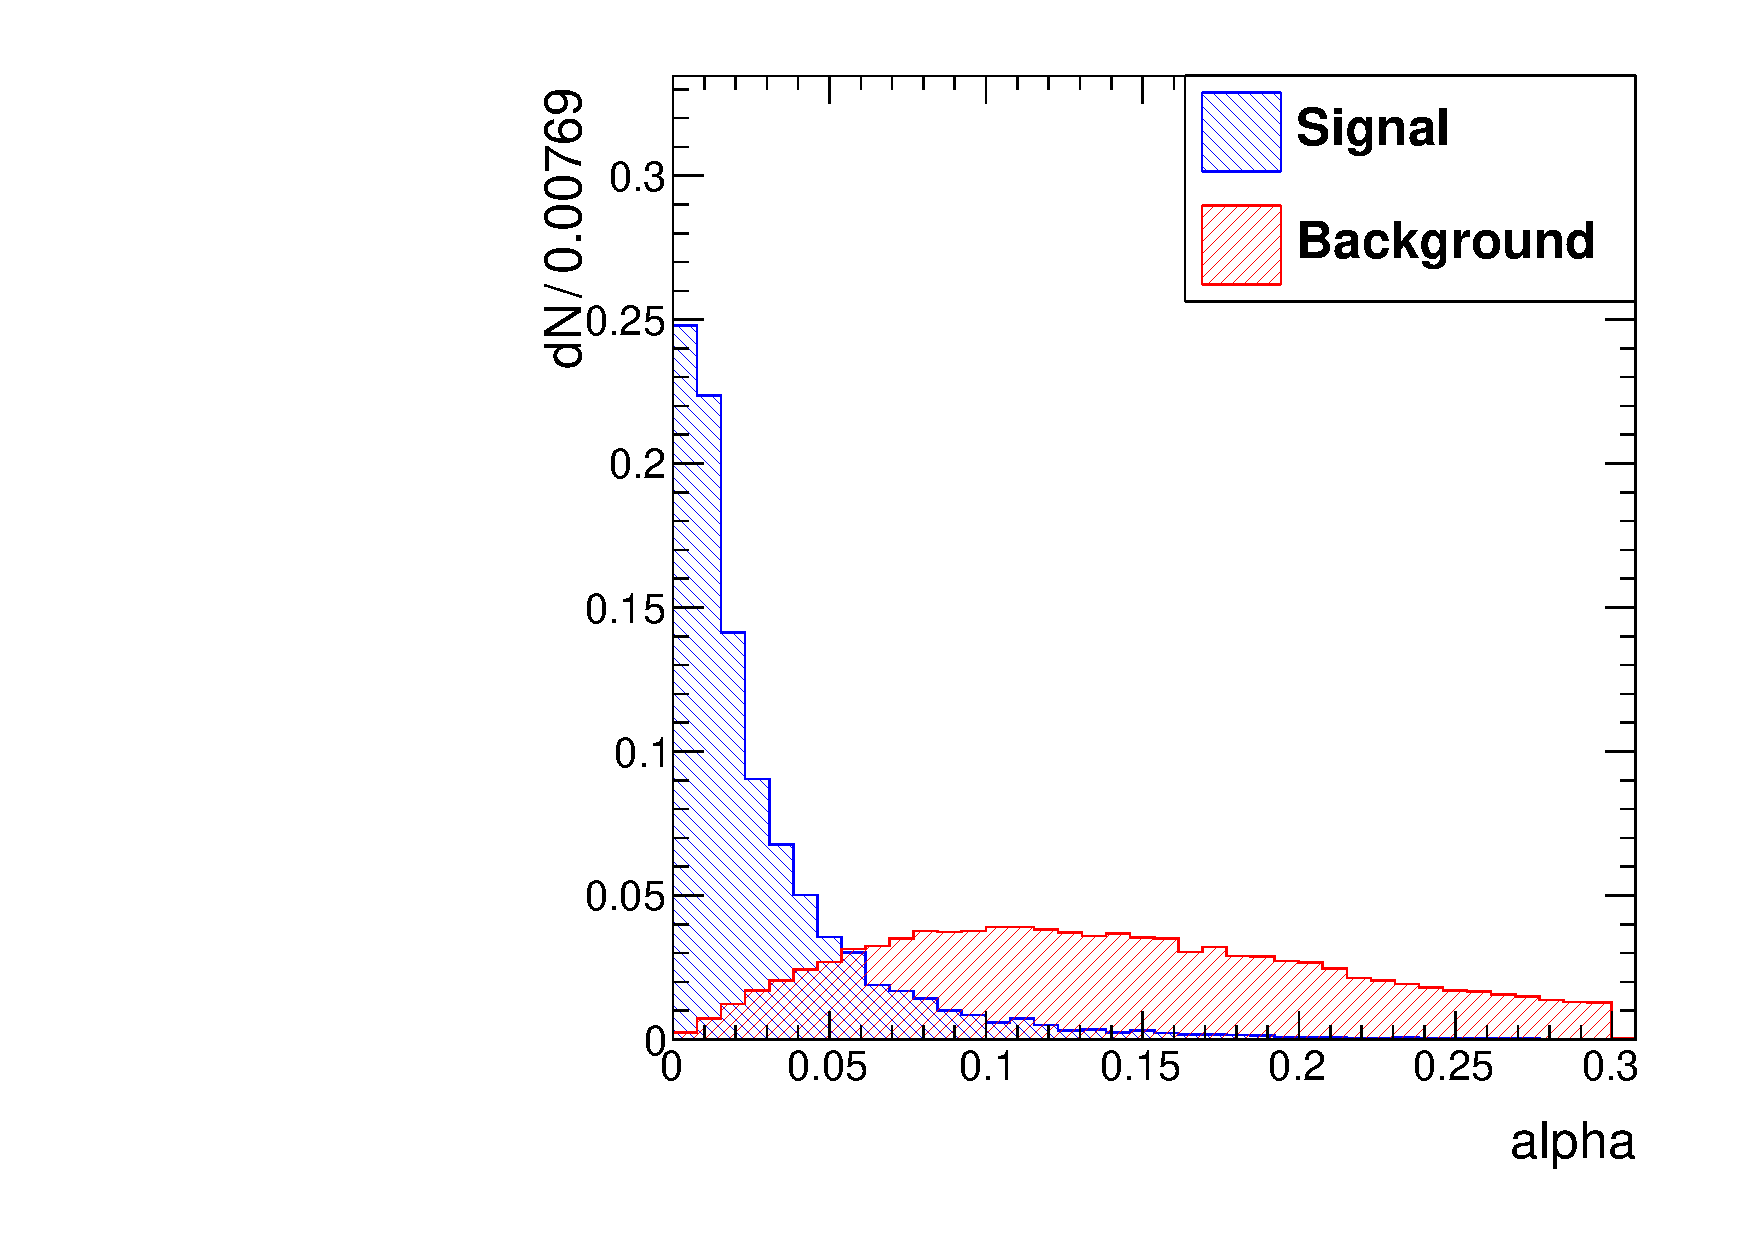
\includegraphics[width=0.3\textwidth]{Figures/alpha_endcaps}
  %\label{fig:alphaEndcaps}
  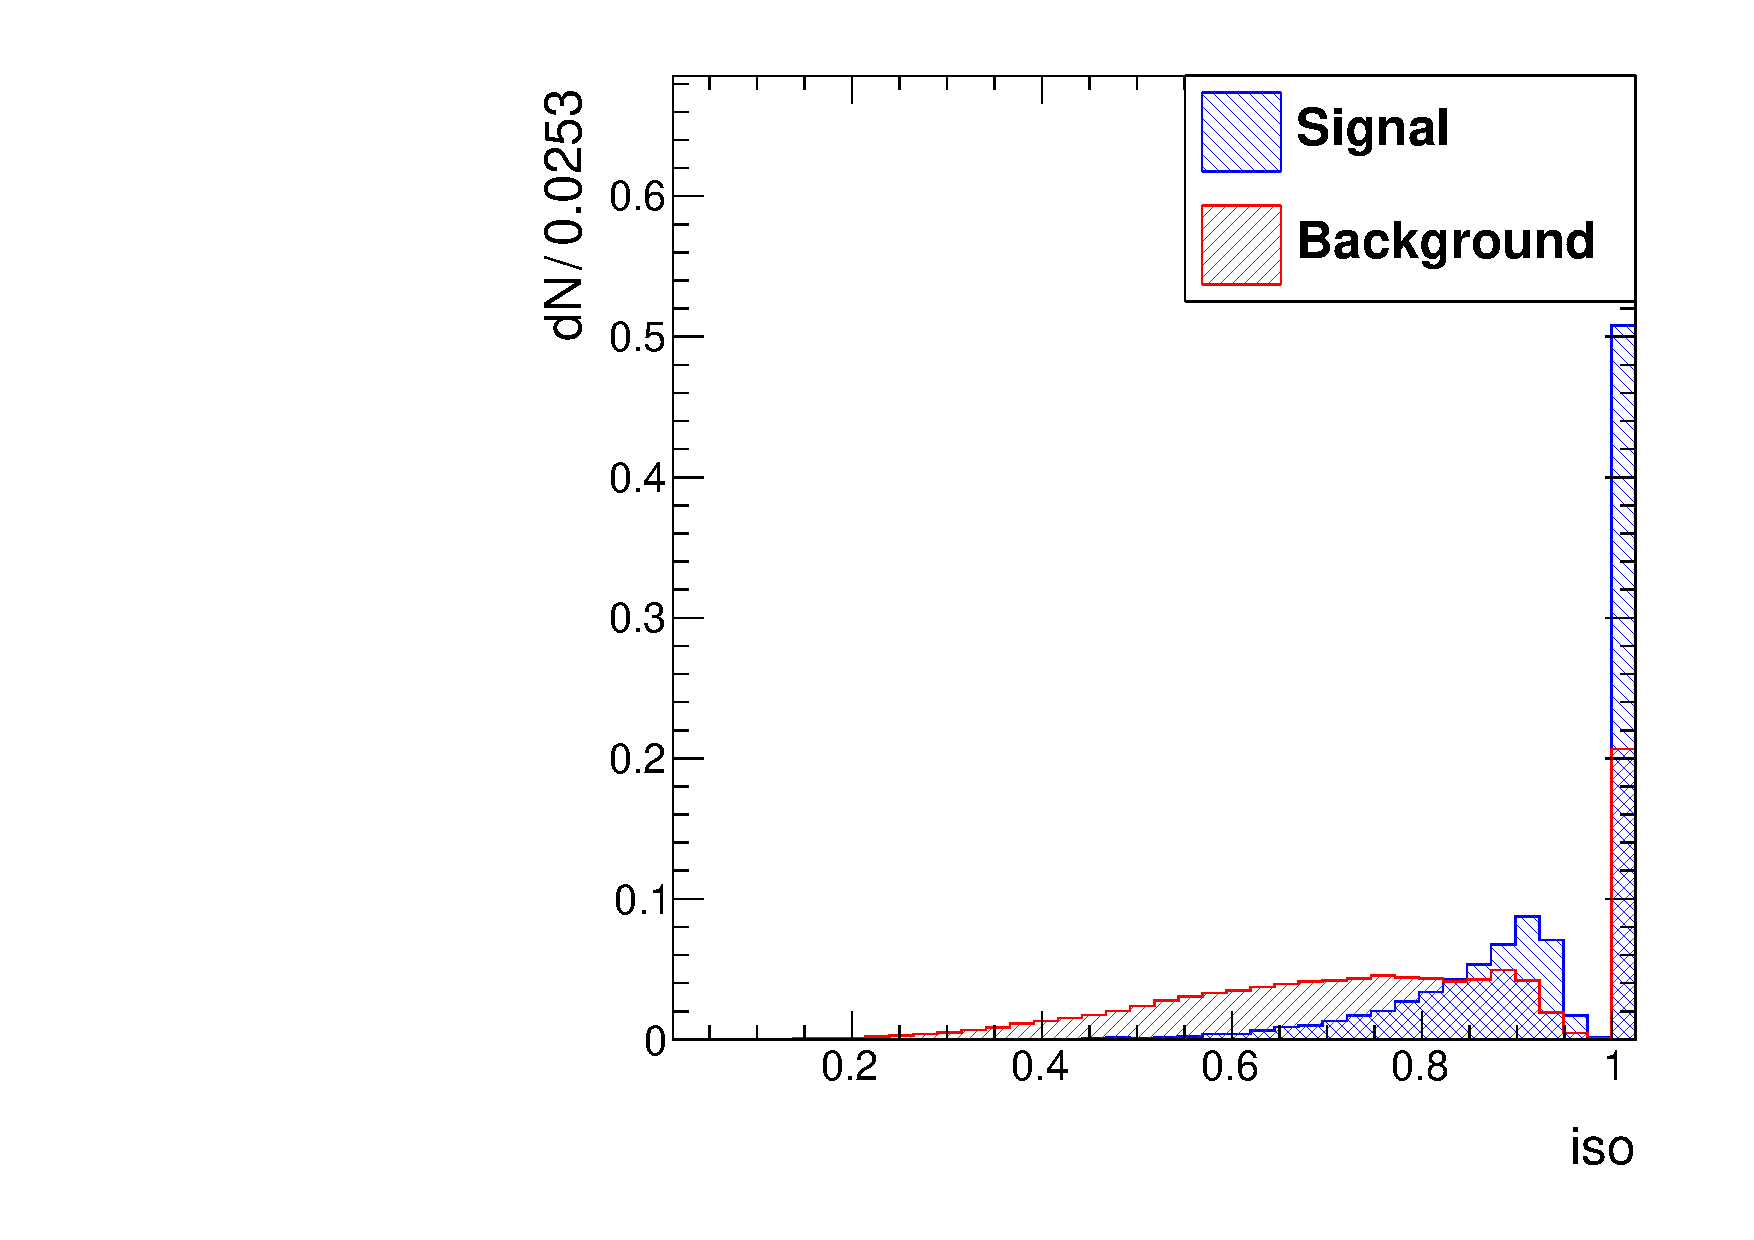
\includegraphics[width=0.3\textwidth]{Figures/iso_endcaps}
  %\label{fig:isoEndcaps}
  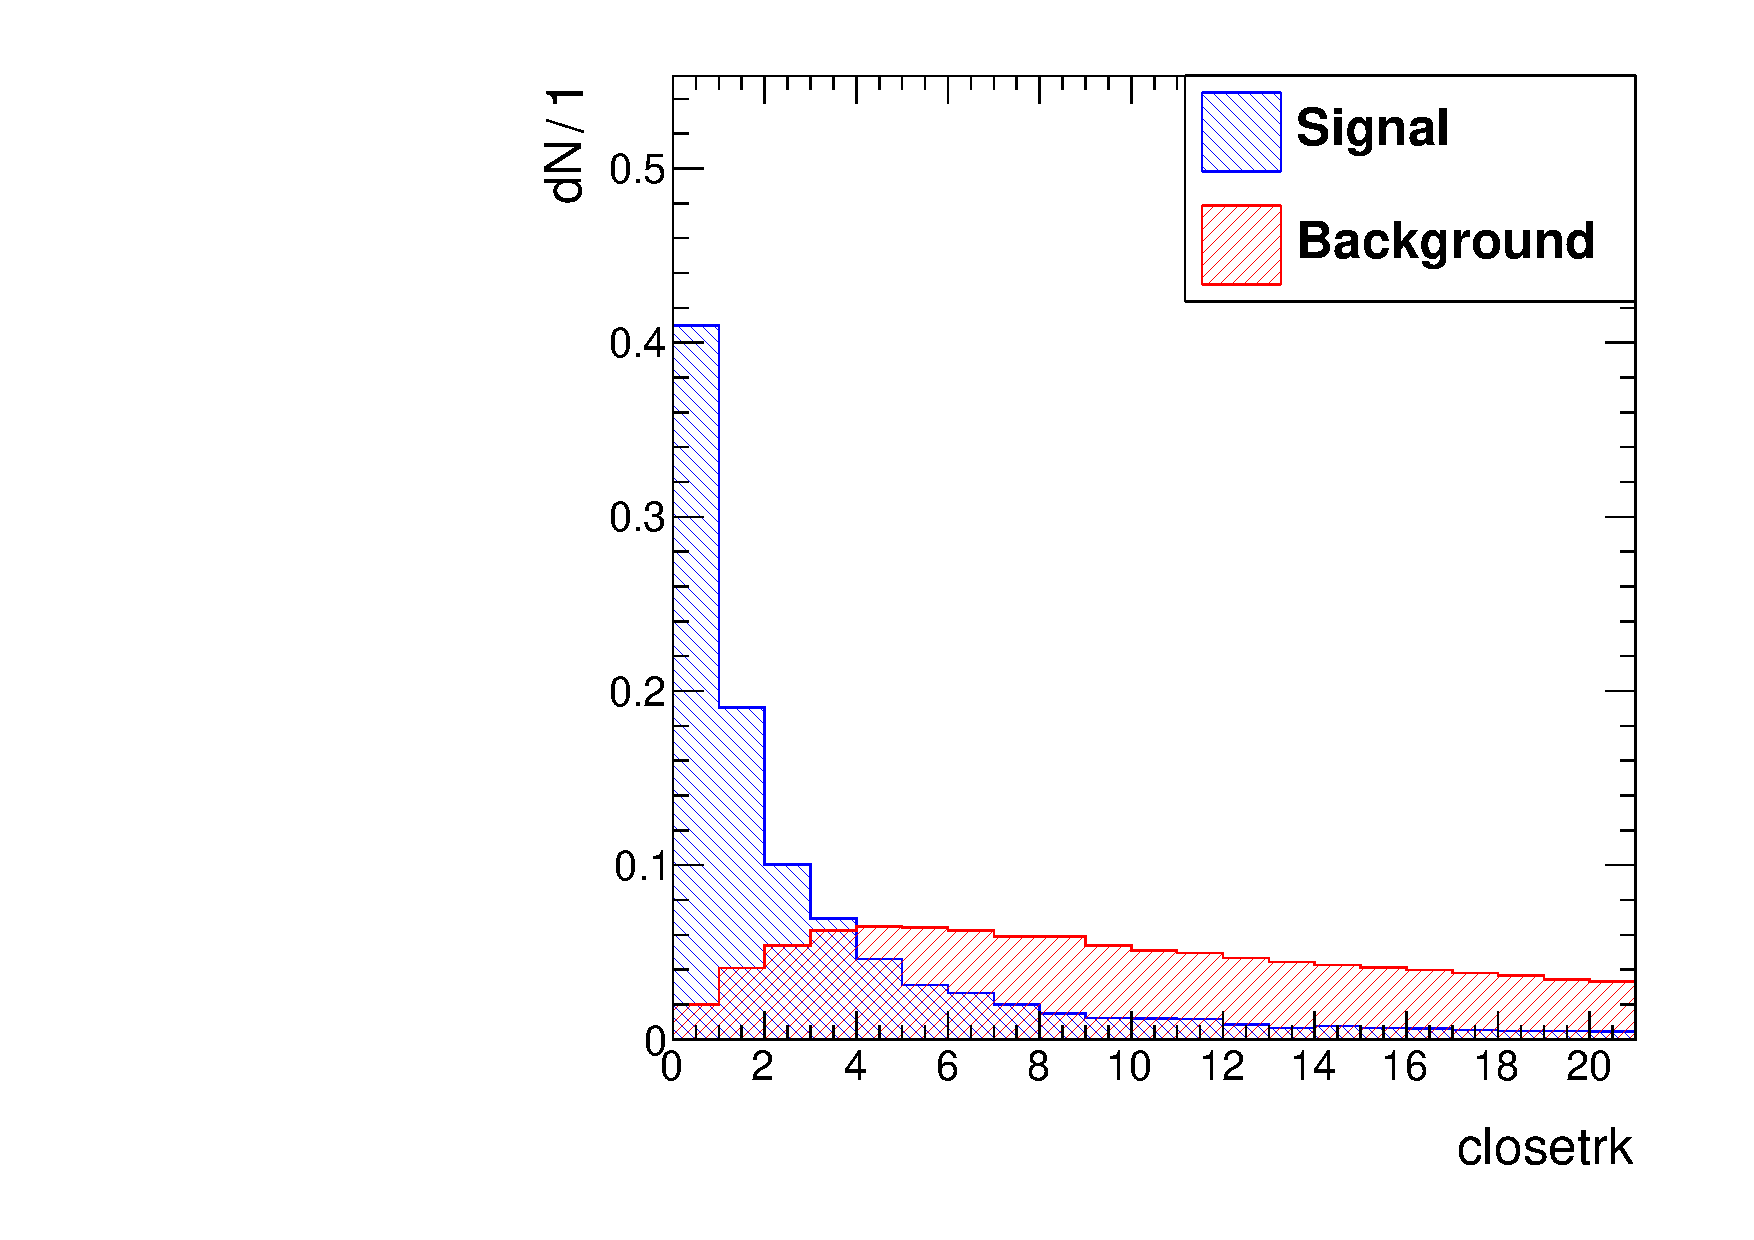
\includegraphics[width=0.3\textwidth]{Figures/closetrk_endcaps}
  %\label{fig:closetrkEndcaps}
  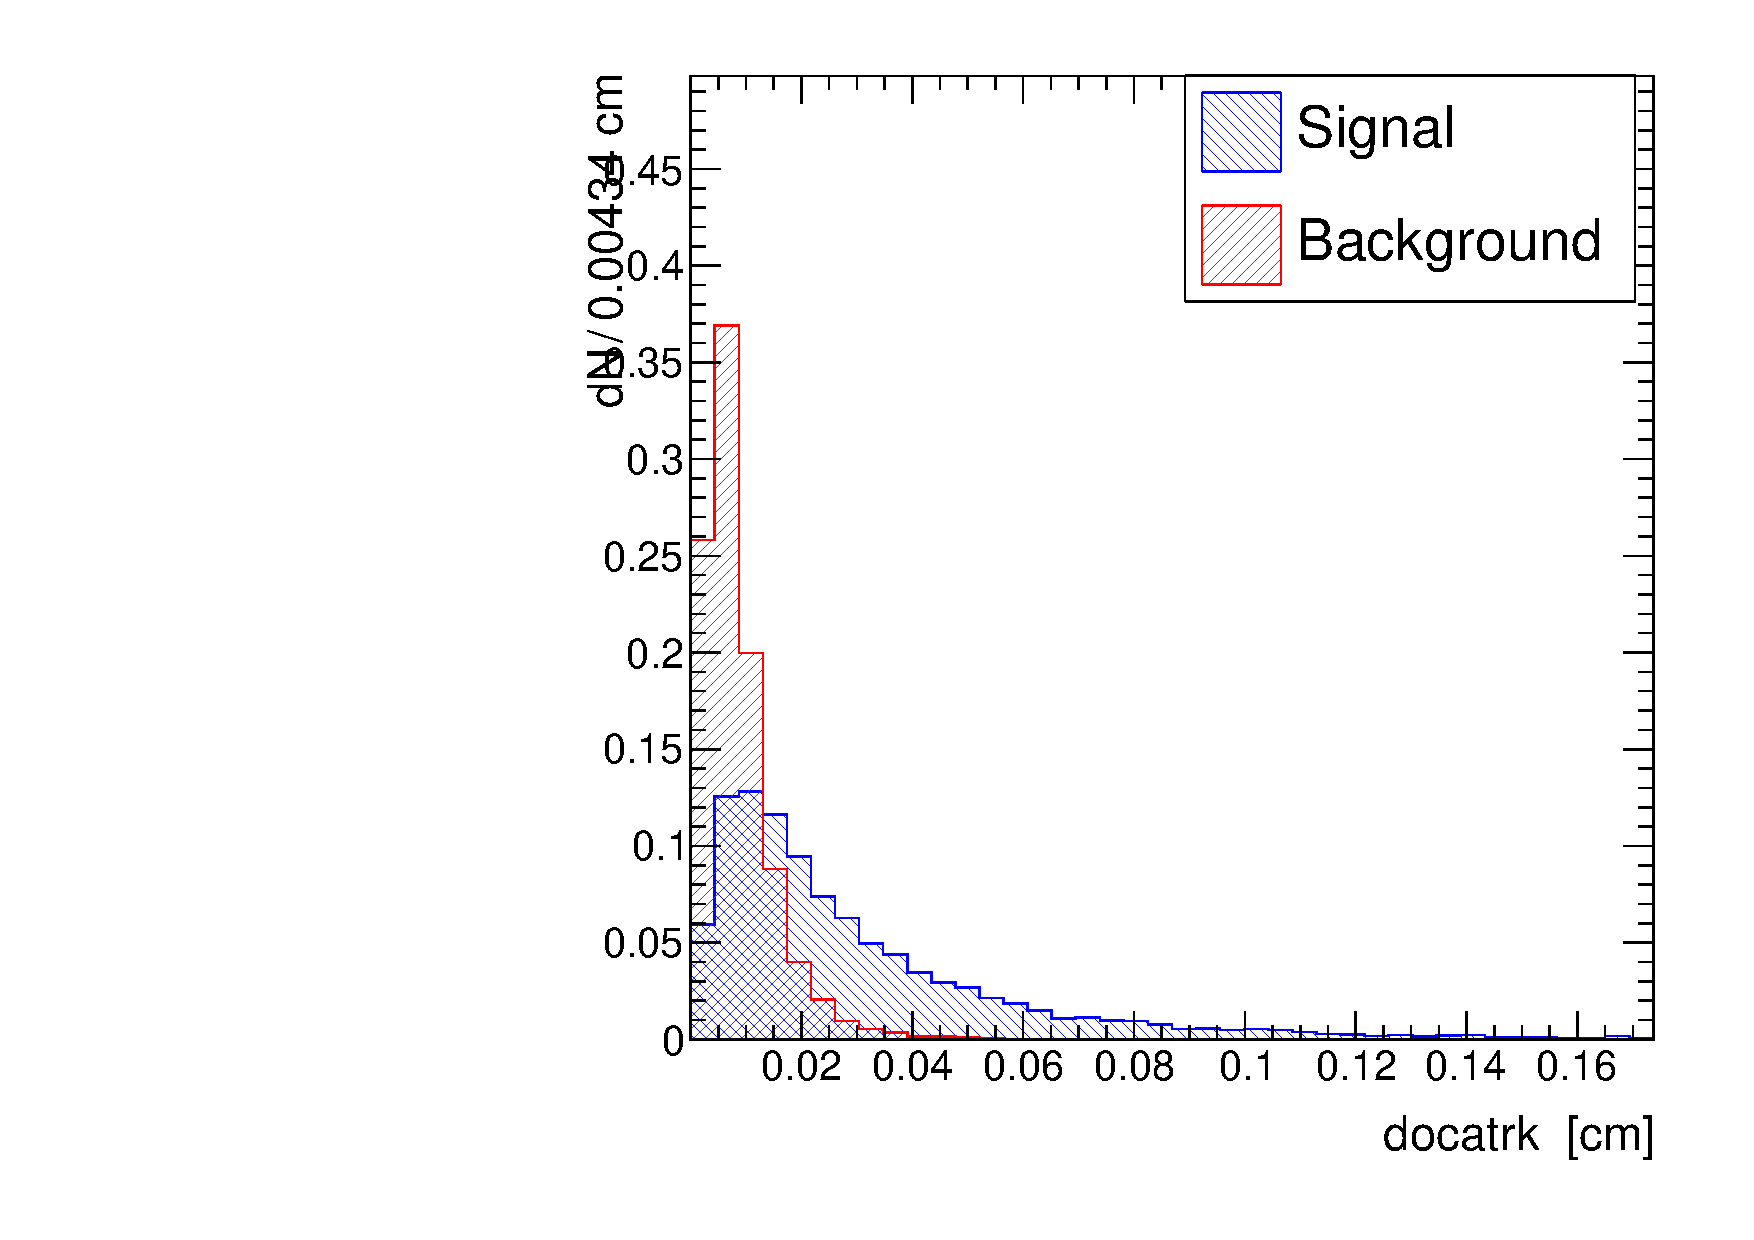
\includegraphics[width=0.3\textwidth]{Figures/docatrk_endcaps}
  %\label{fig:docatrkEndcaps}
  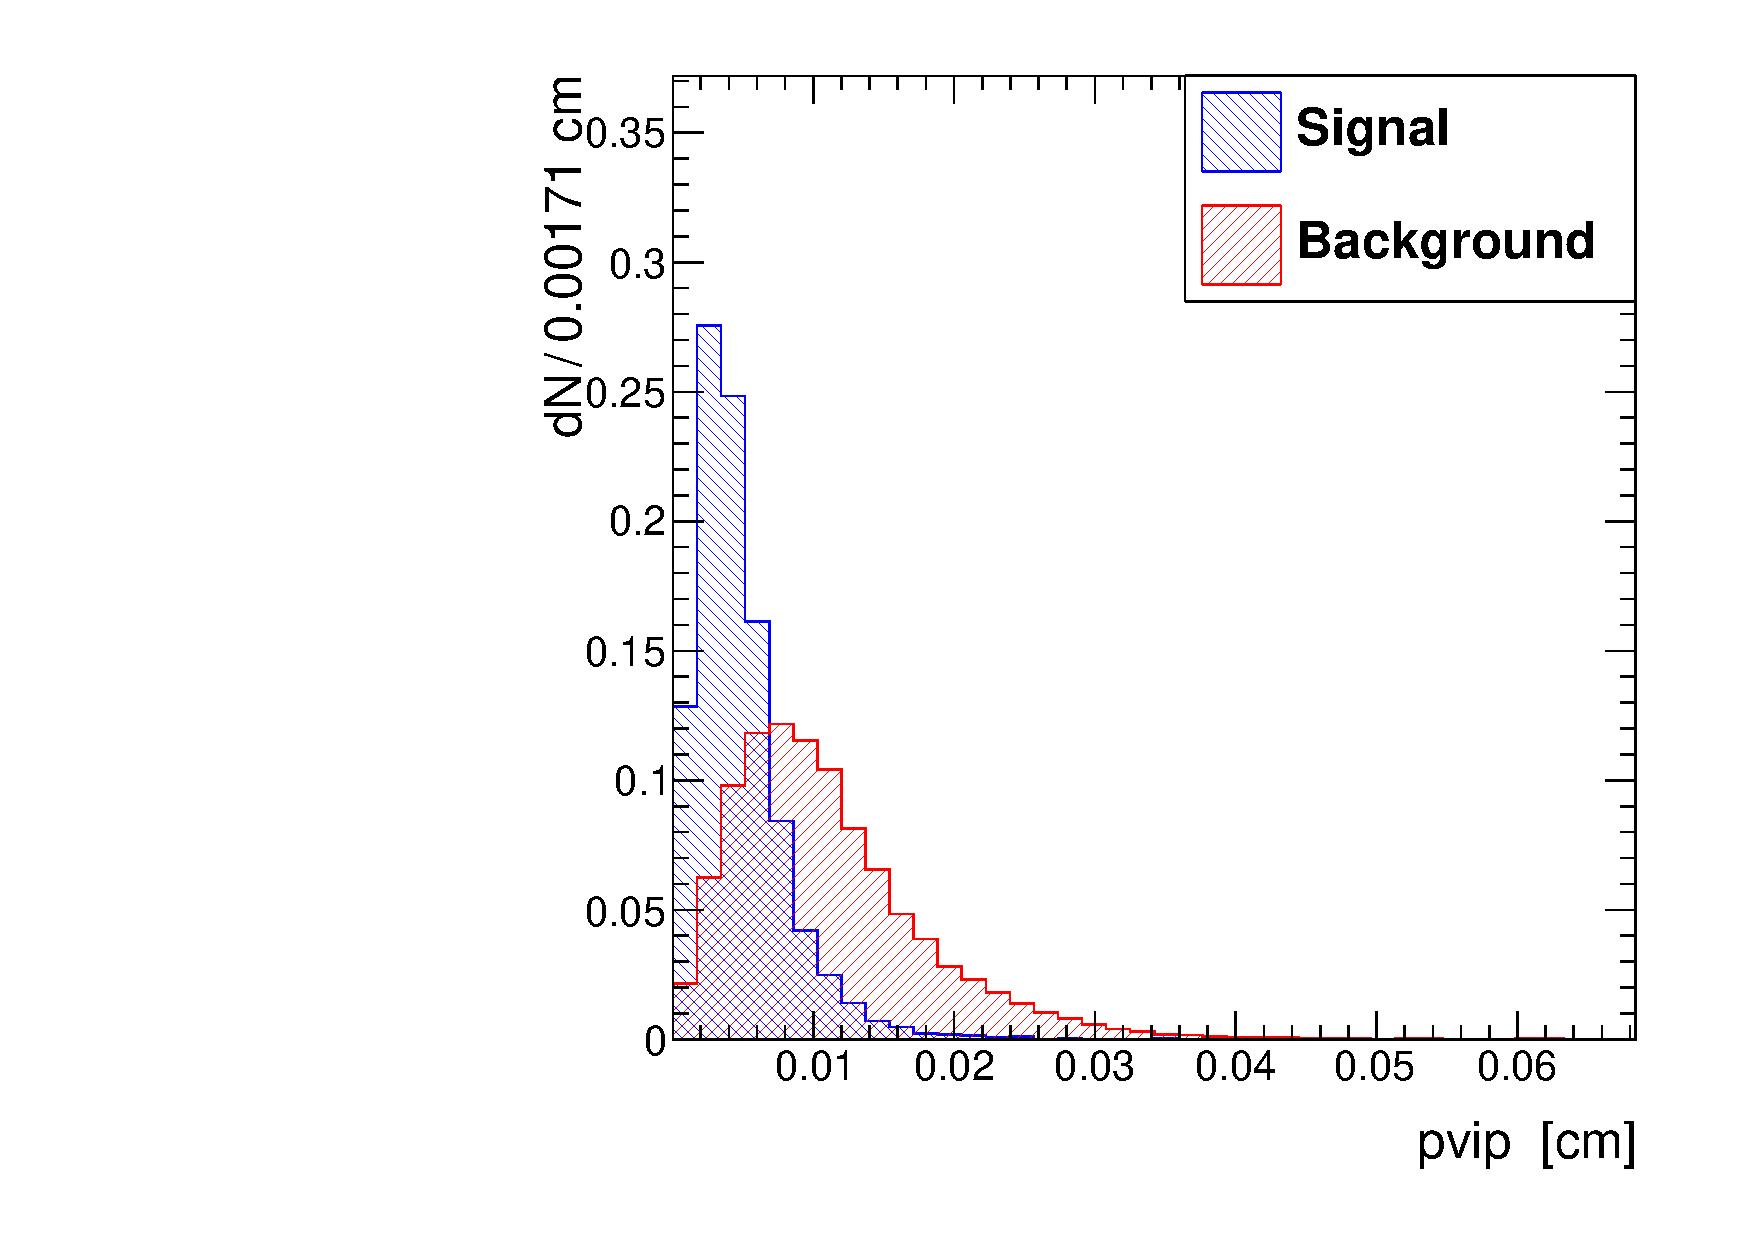
\includegraphics[width=0.3\textwidth]{Figures/pvip_endcaps}
  %\label{fig:pvipEndcaps}
  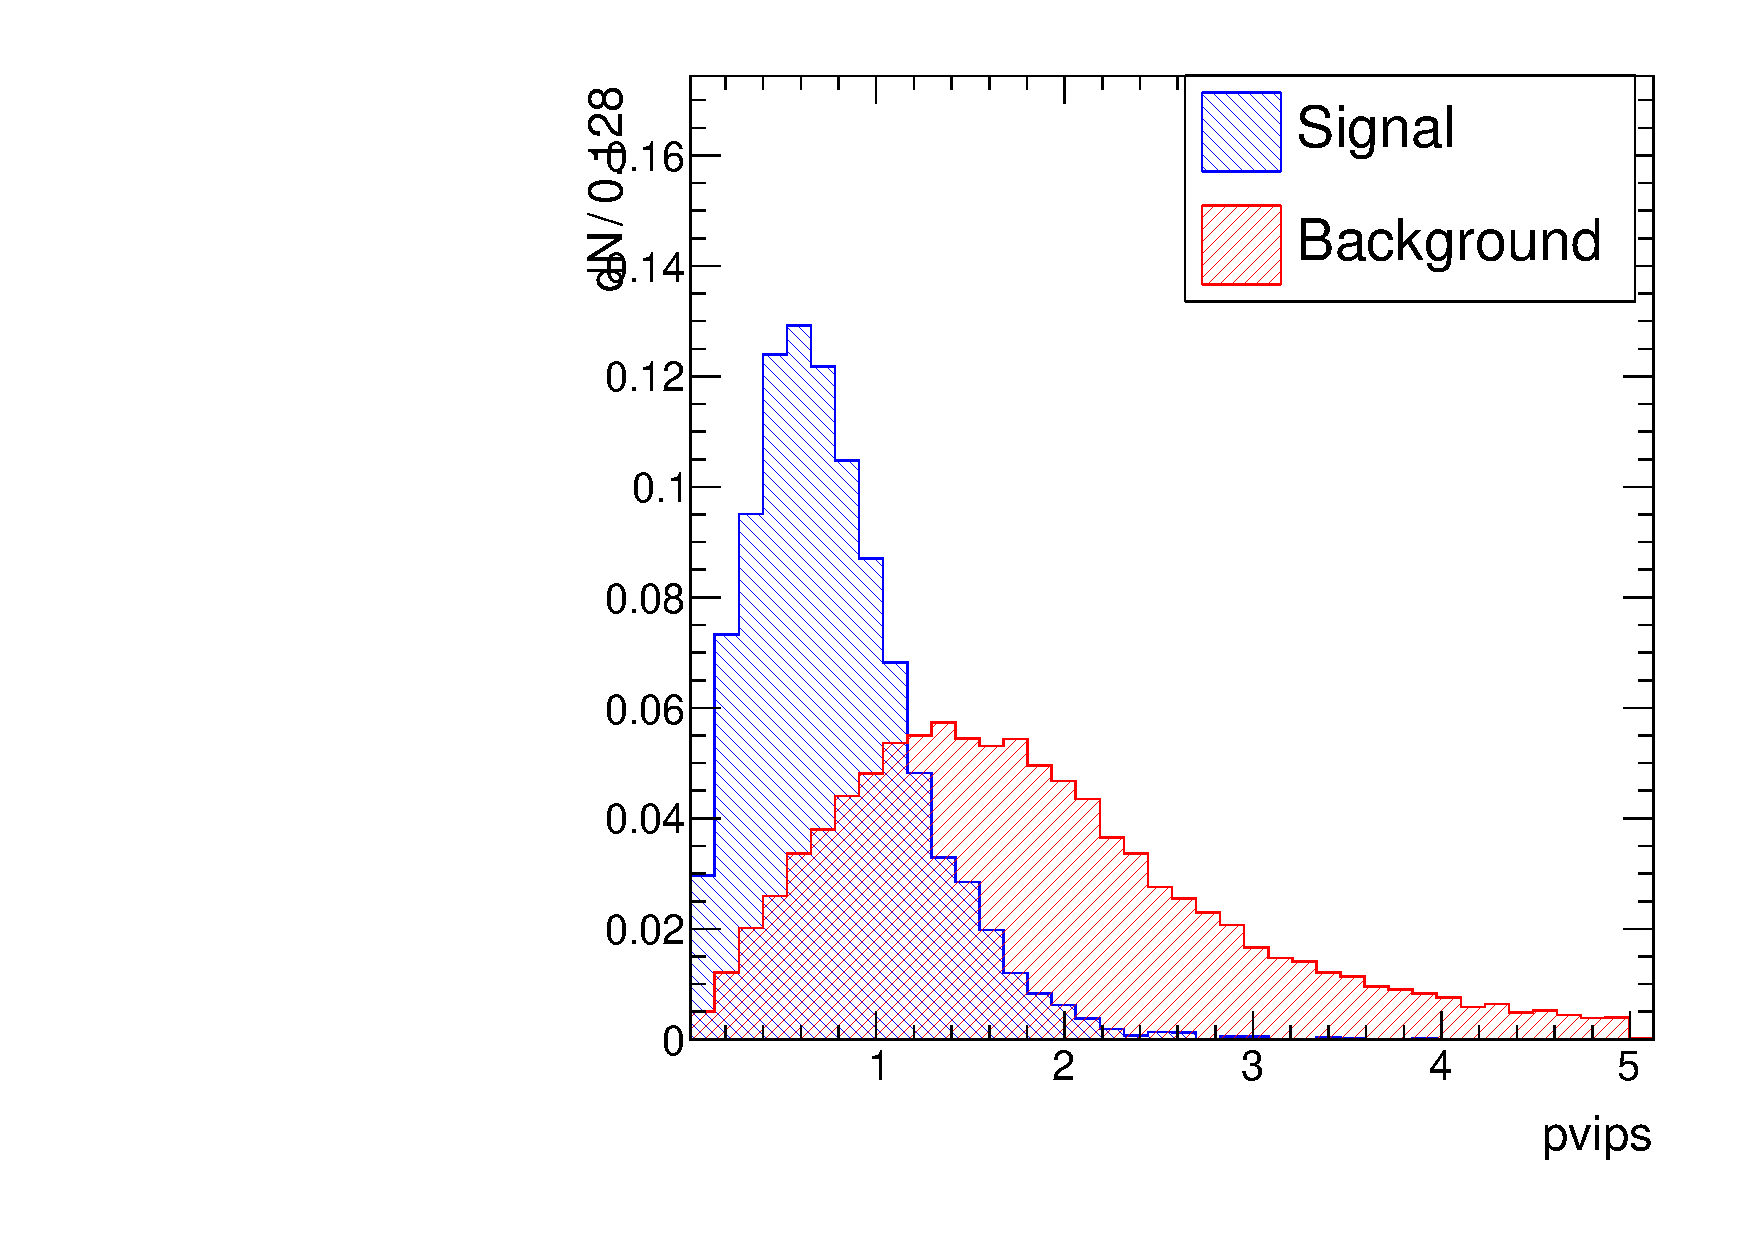
\includegraphics[width=0.3\textwidth]{Figures/pvips_endcaps}
  %\label{fig:pvipsEncaps}
  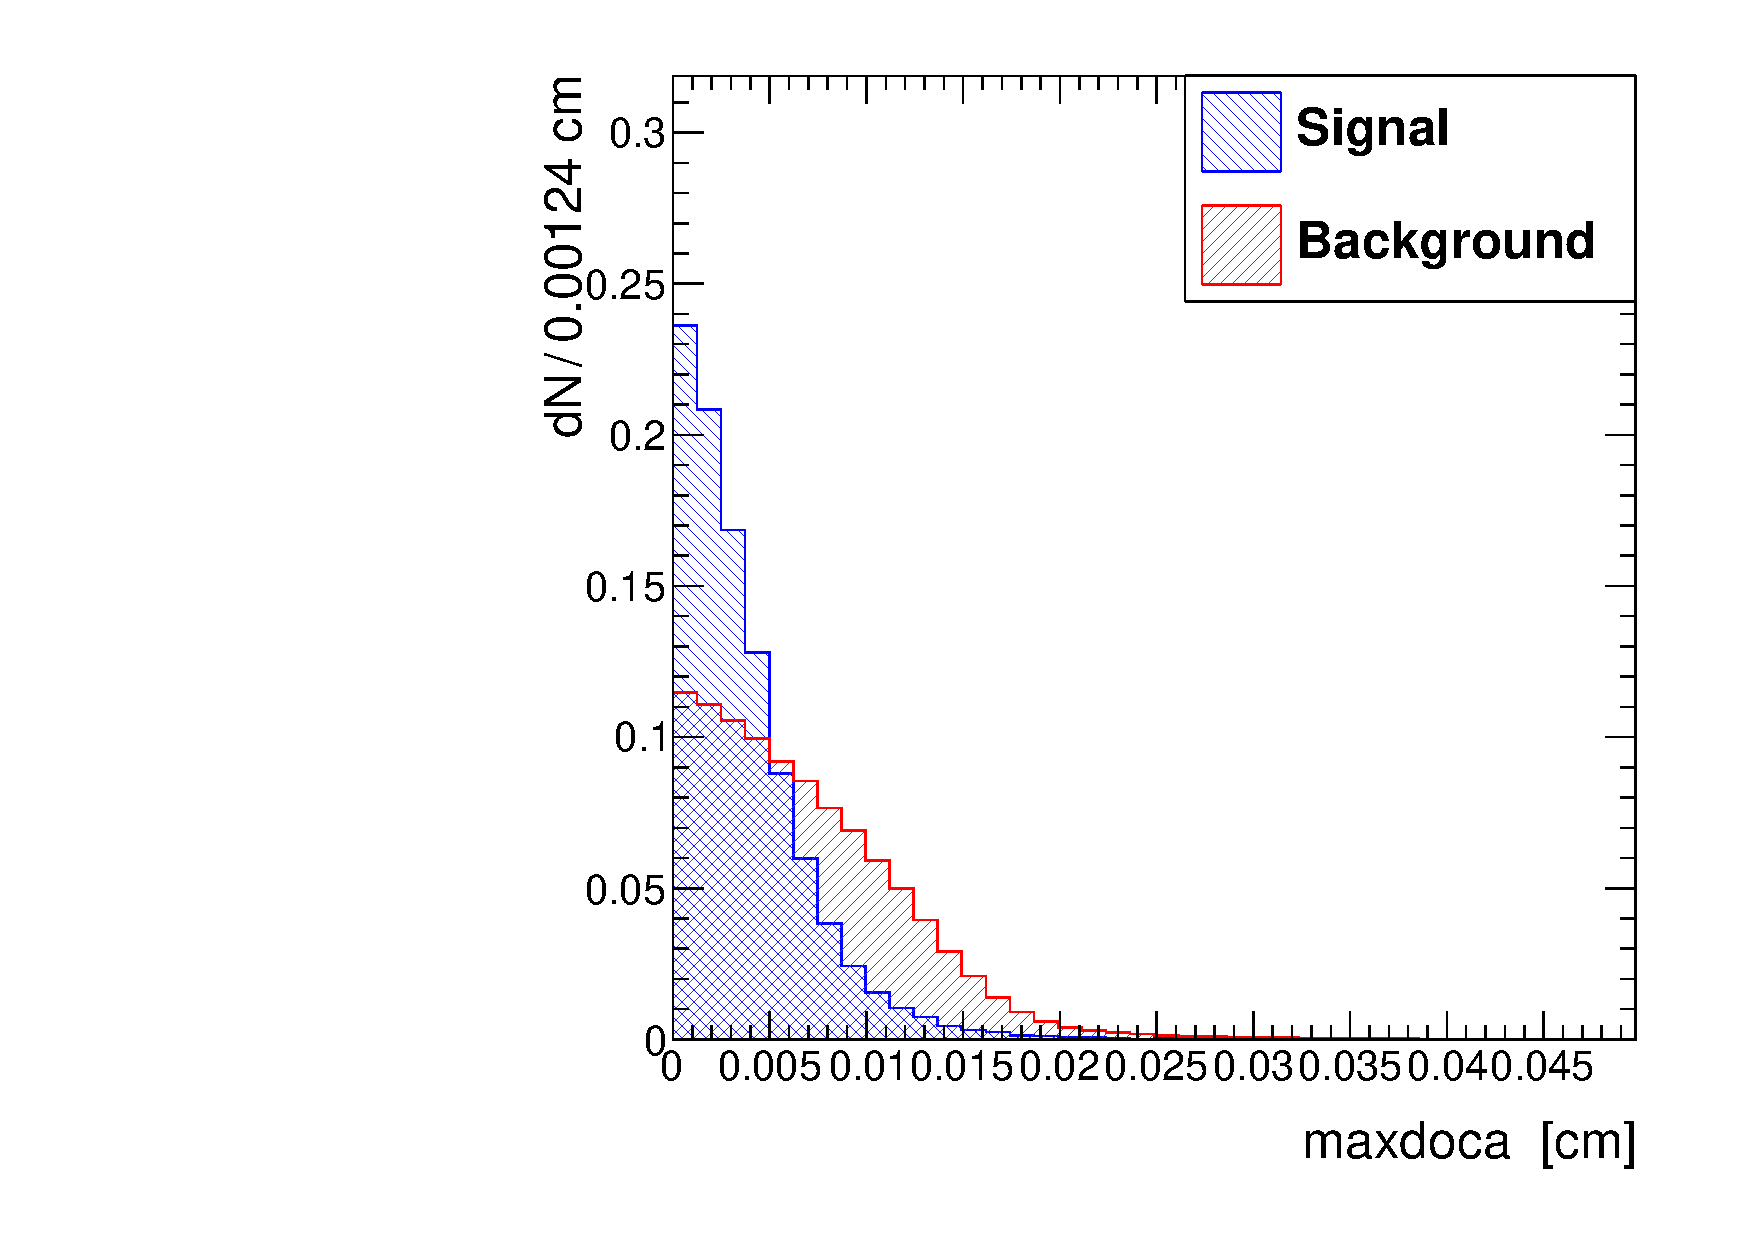
\includegraphics[width=0.3\textwidth]{Figures/maxdoca_endcaps}
  %\label{fig:maxdocaEndcaps}
  \caption{Standard TMVA plot of the input variables for the endcaps BDT for signal (blue) and background (red). The background is extracted from data dimuon sidebands.}
  \label{fig:TMVAPlotsEndcaps}
\end{figure}



\subsection{variable ranking and correlations}

\begin{figure}
  \centering
  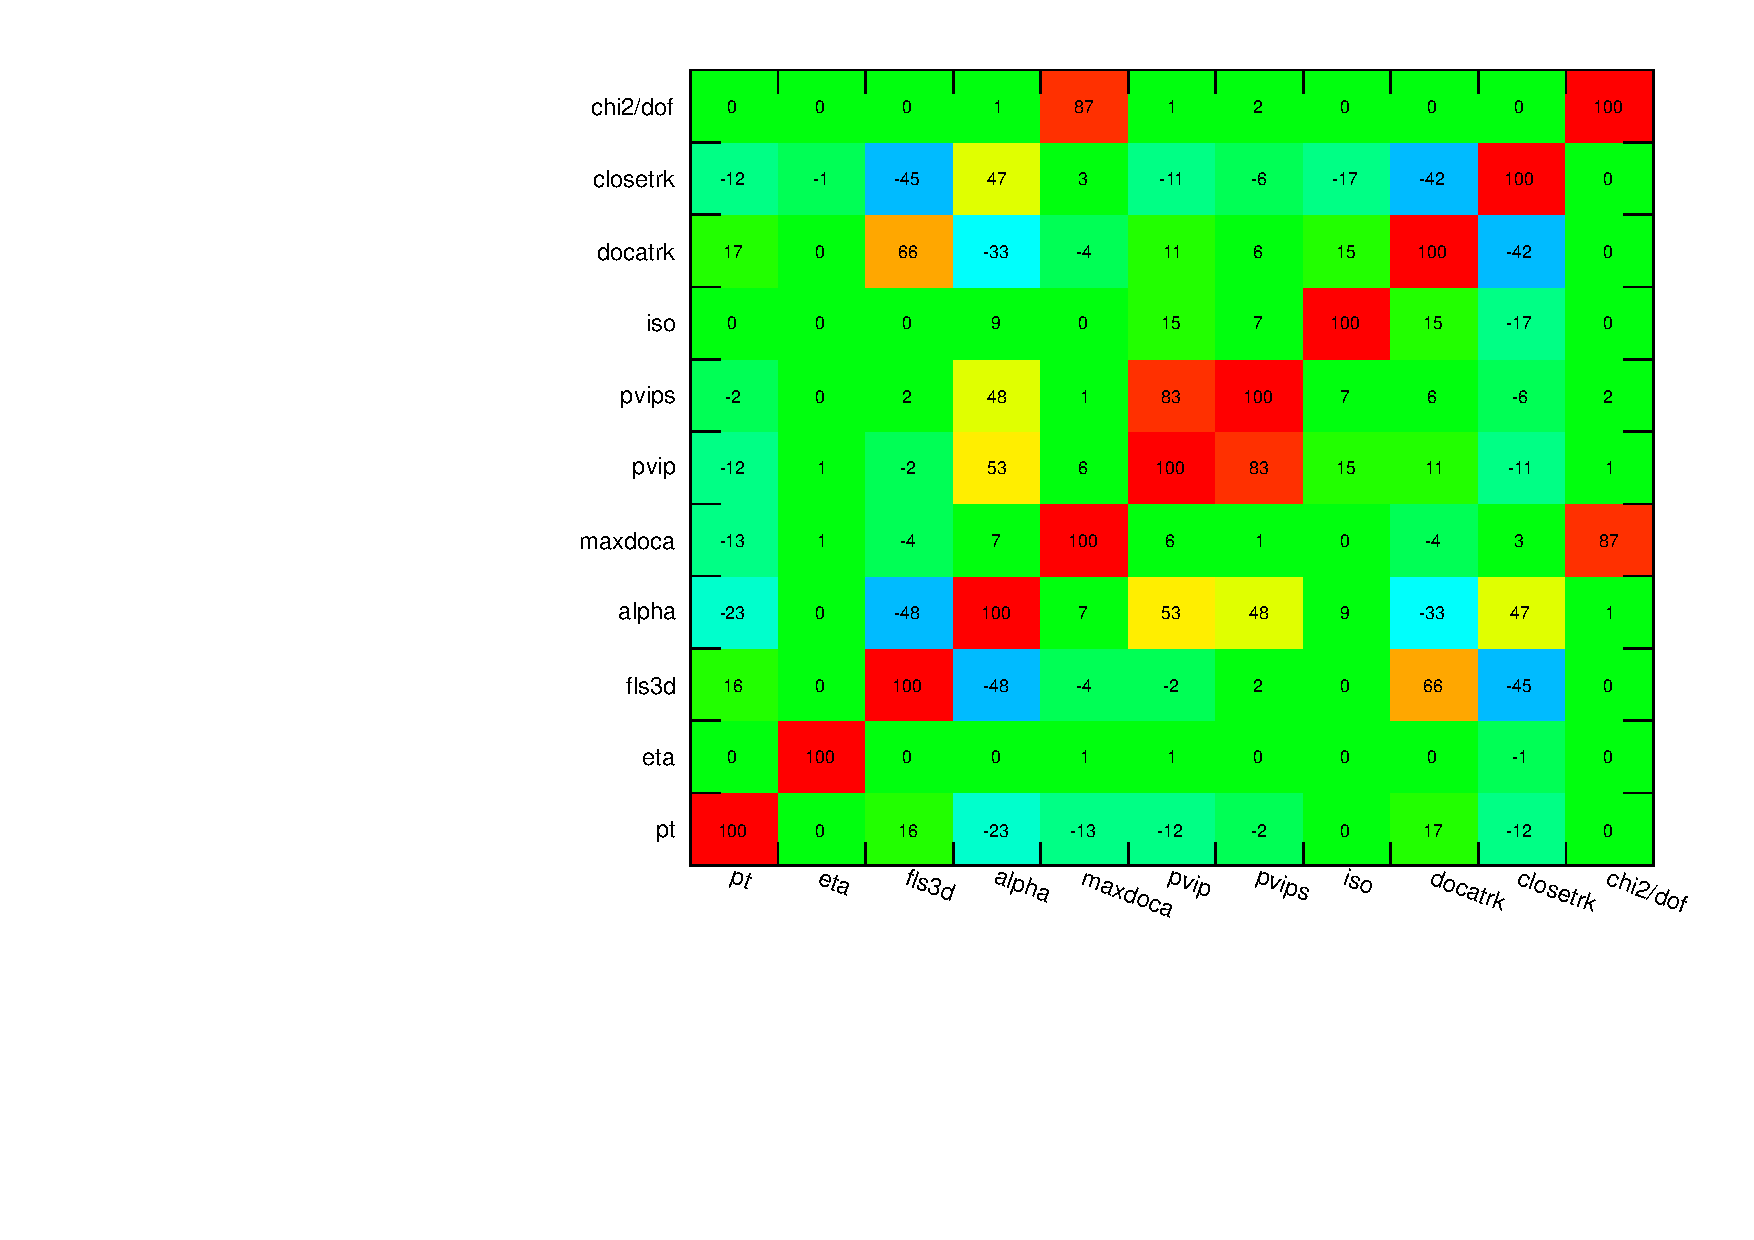
\includegraphics[width=0.45\textwidth]{Figures/correlationMatrixS_barrel}
  \label{fig:matrixSBarrel}
  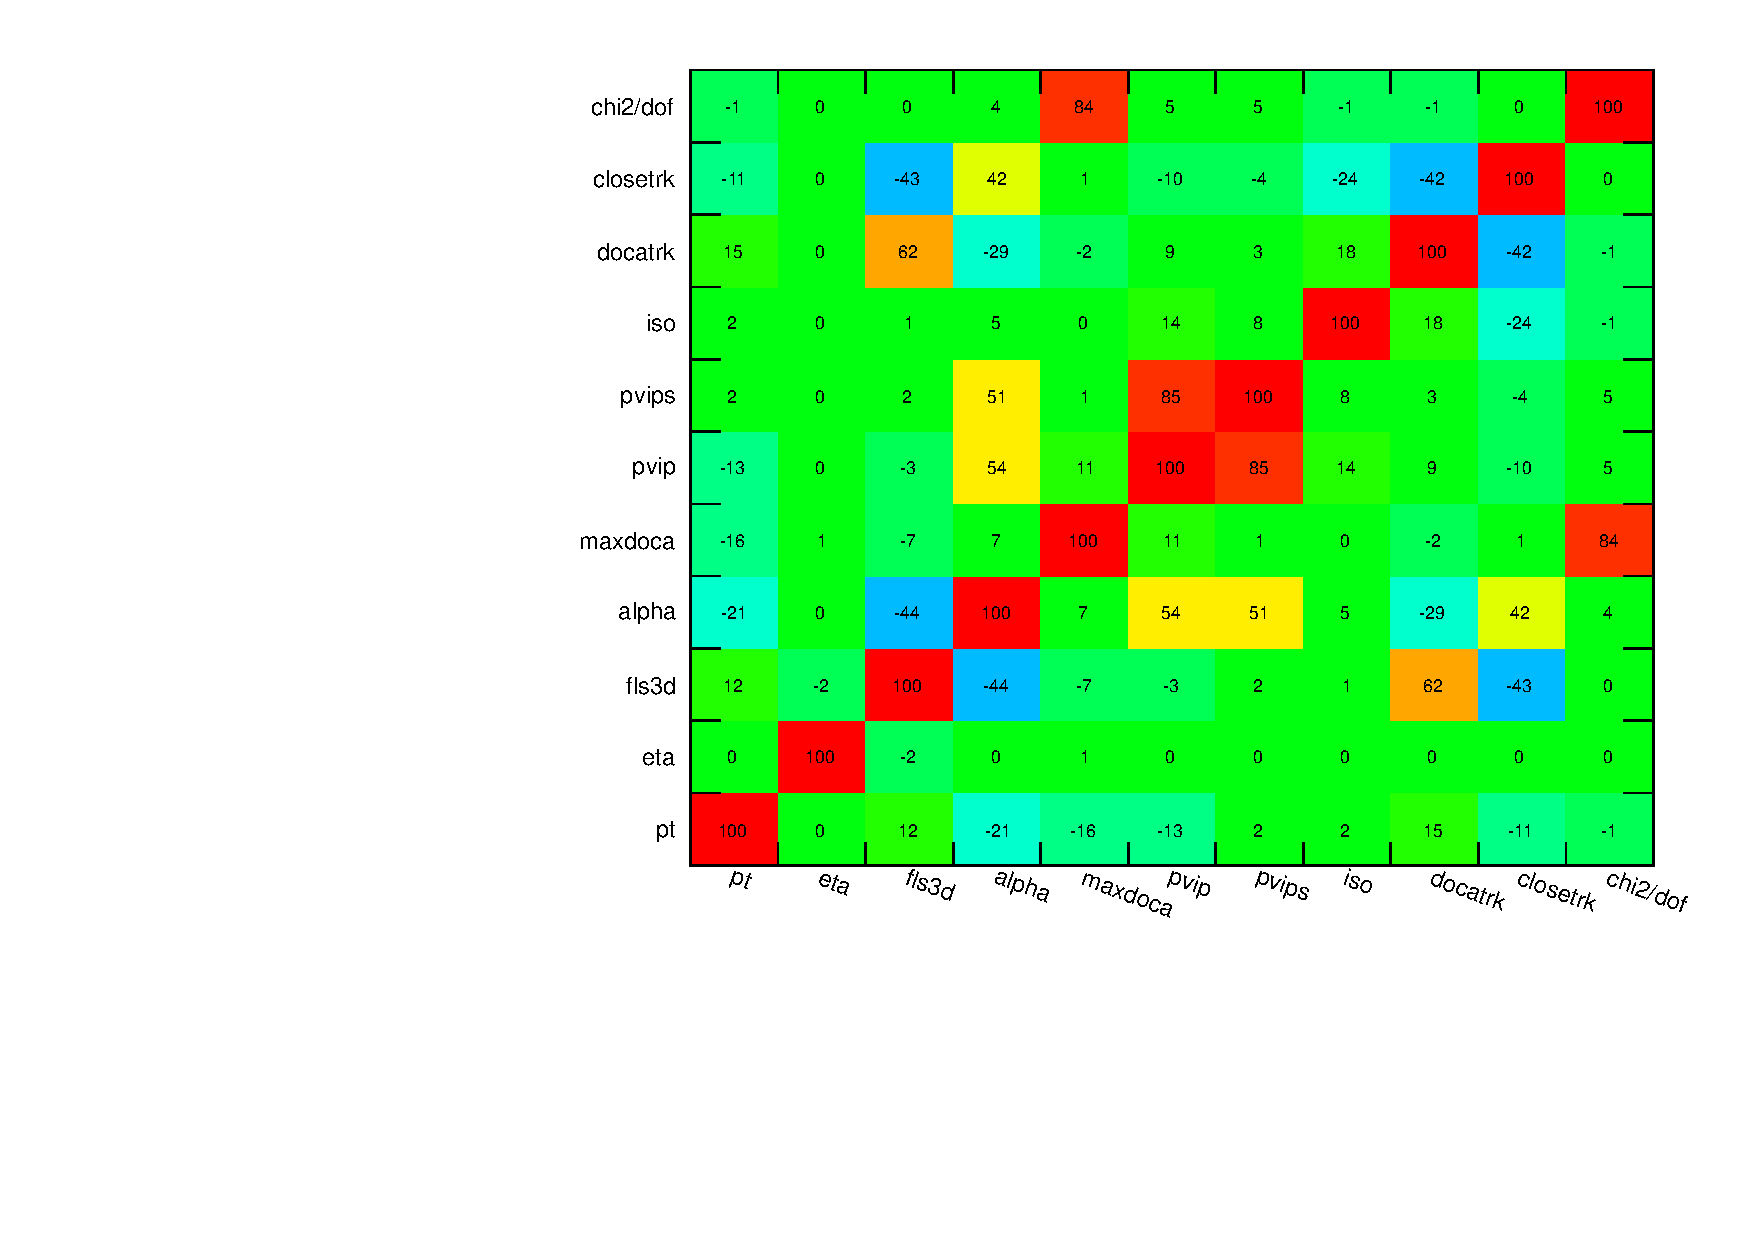
\includegraphics[width=0.45\textwidth]{Figures/correlationMatrixS_endcaps}
  \label{fig:matrixSEndcaps}
  \caption{Correlation matrix for signal events in the barrel (left) and the endcap (right).}
  \label{fig:correlationMatricesSignal}
\end{figure}

\begin{figure}
  \centering
  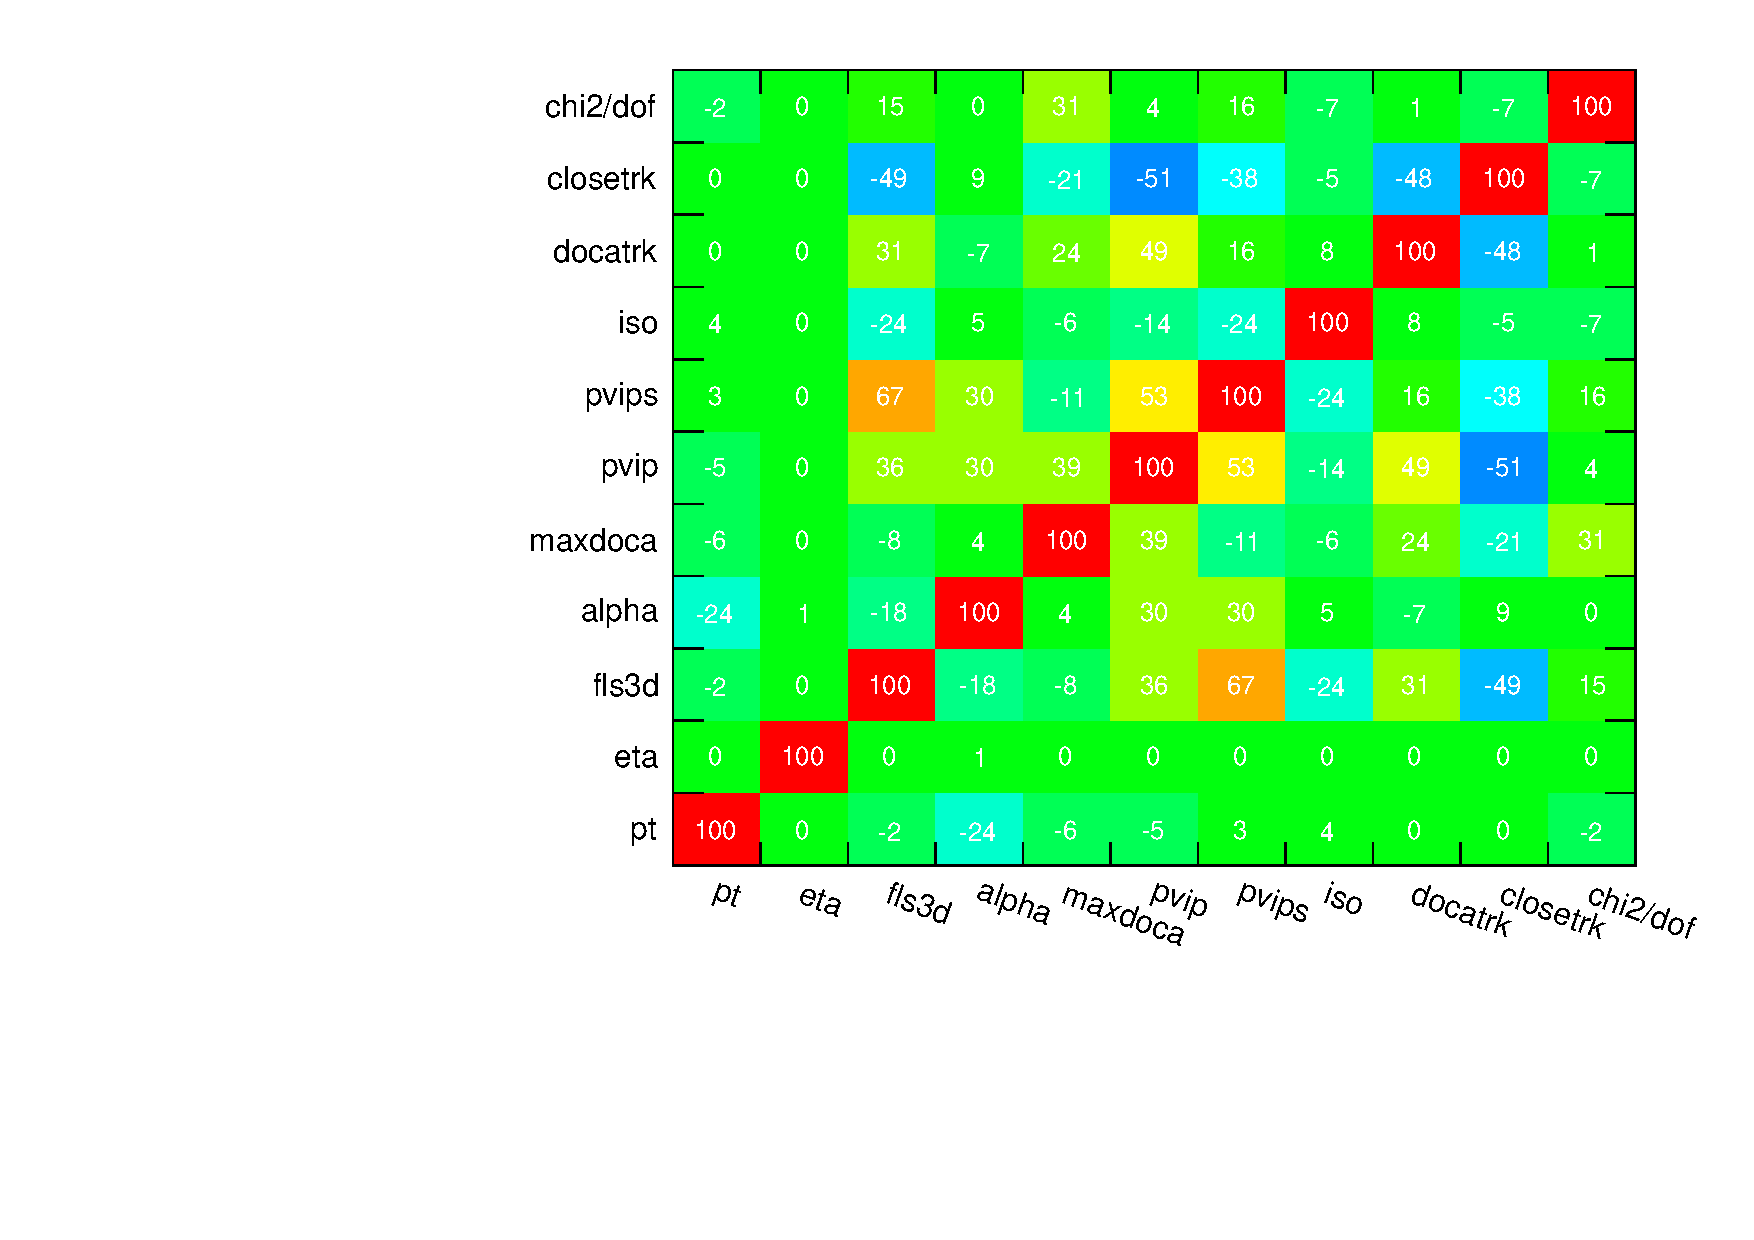
\includegraphics[width=0.45\textwidth]{Figures/correlationMatrixB_barrel}
  \label{fig:matrixBBarrel}
  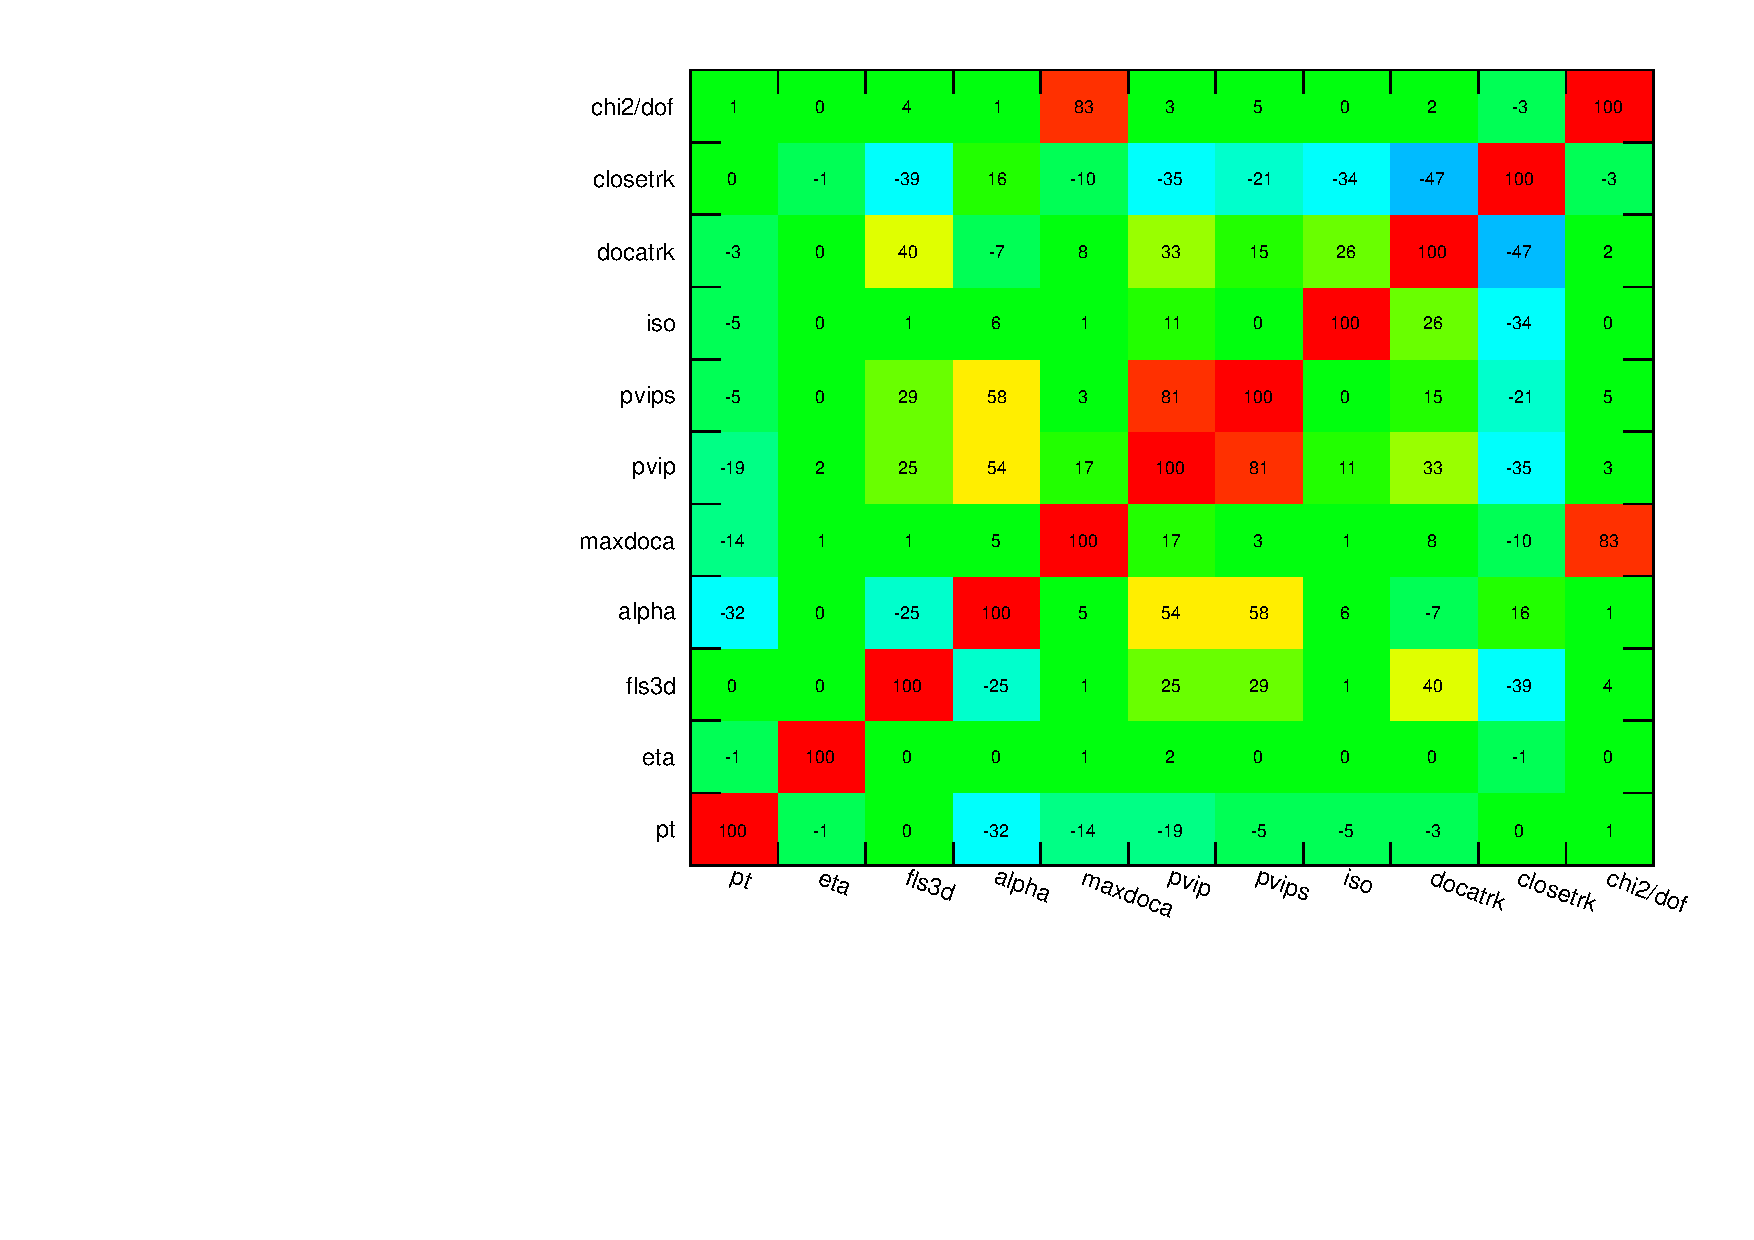
\includegraphics[width=0.45\textwidth]{Figures/correlationMatrixB_endcaps}
  \label{fig:matrixBEndcaps}
  \caption{Correlation matrix for background events in the barrel (left) and the endcap (right).}
  \label{fig:correlationMatricesBackground}
\end{figure}

Tables \ref{tab:datasetsbarrelIdTransformation} and \ref{tab:datasetsendcapsIdTransformation} show the ranking of variables before
the BDT training.

\input{Tables/ranking_barrel_IdTransformation.txt}
\input{Tables/ranking_endcaps_IdTransformation.txt}


%what code prodcues these?
%\begin{figure}
  \centering
  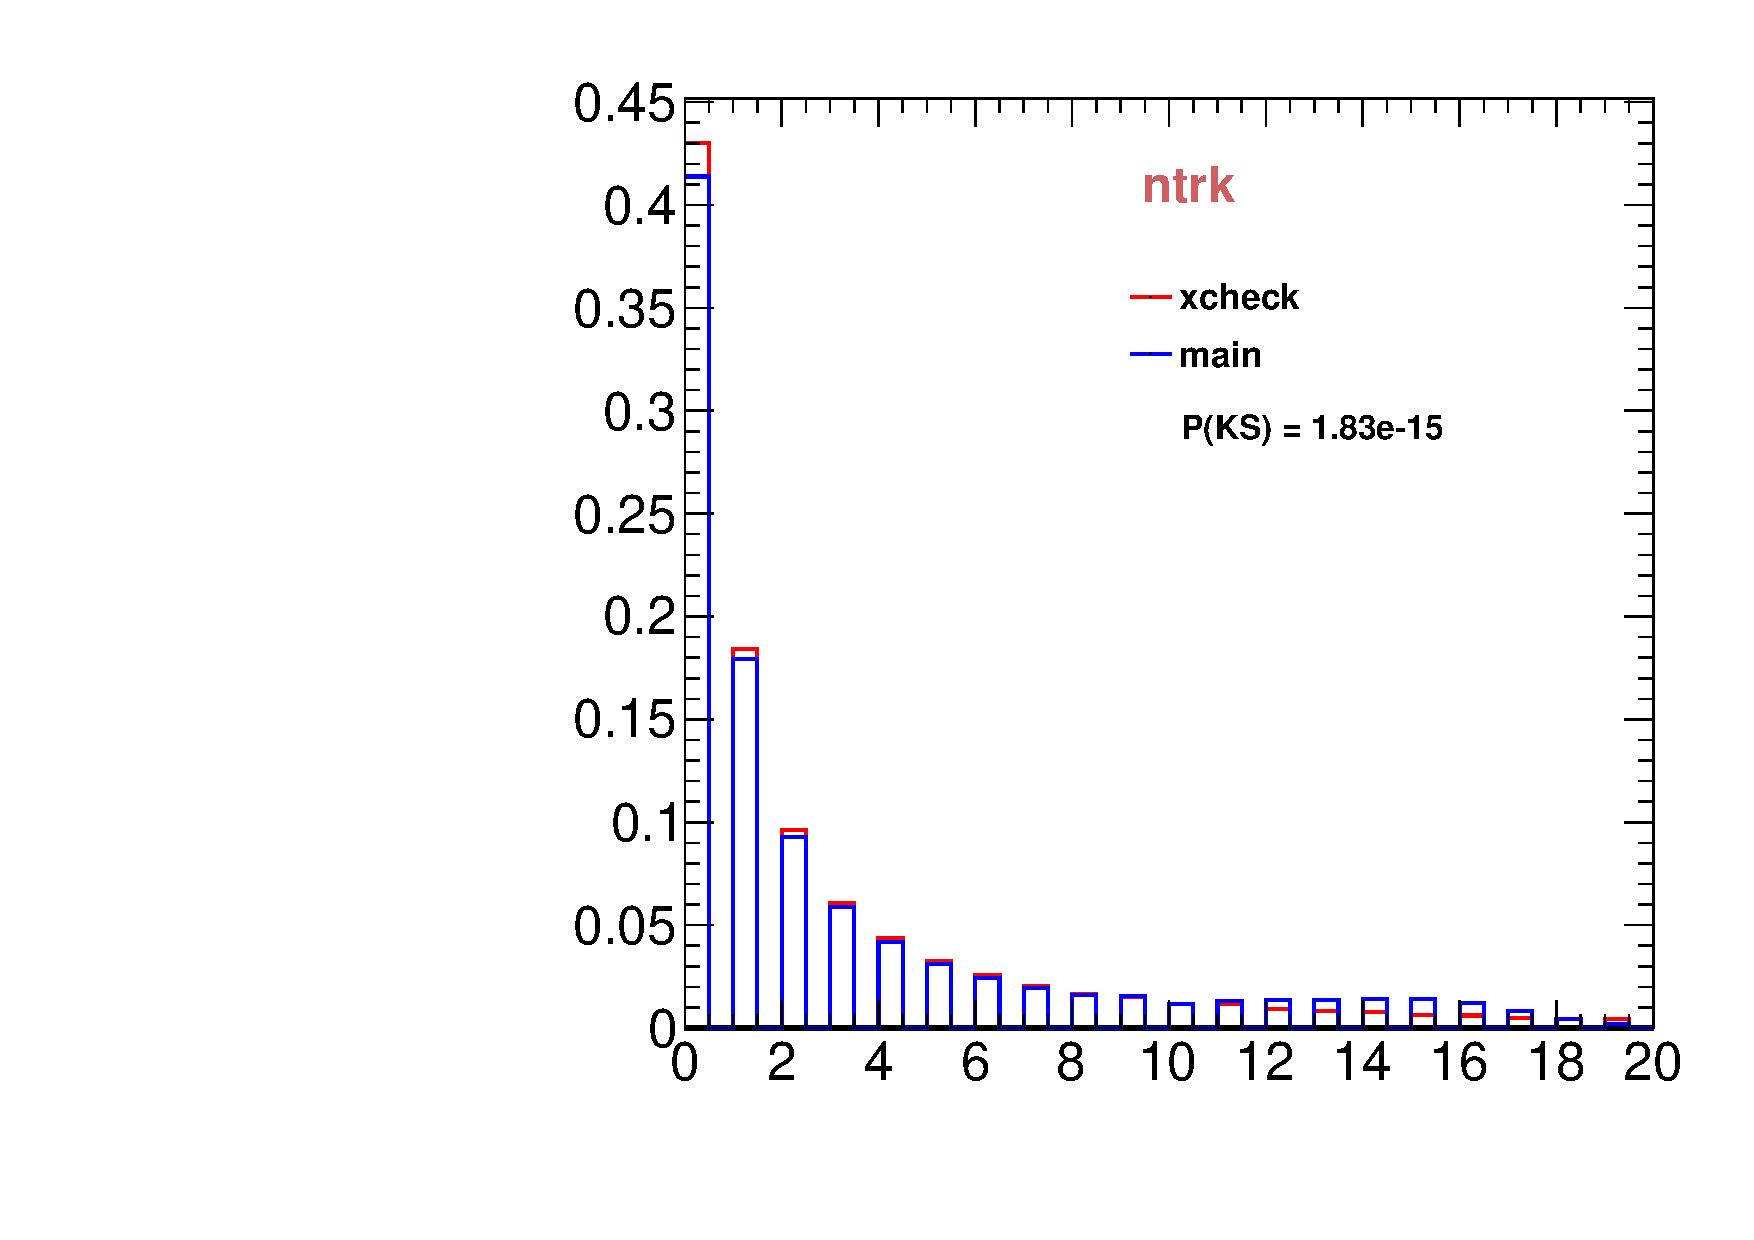
\includegraphics[width=0.3\textwidth]{Figures/VariablesComparison/MC_barrel_figs/closetrk}
  %\label{fig:MC_barrel_closetrk}
  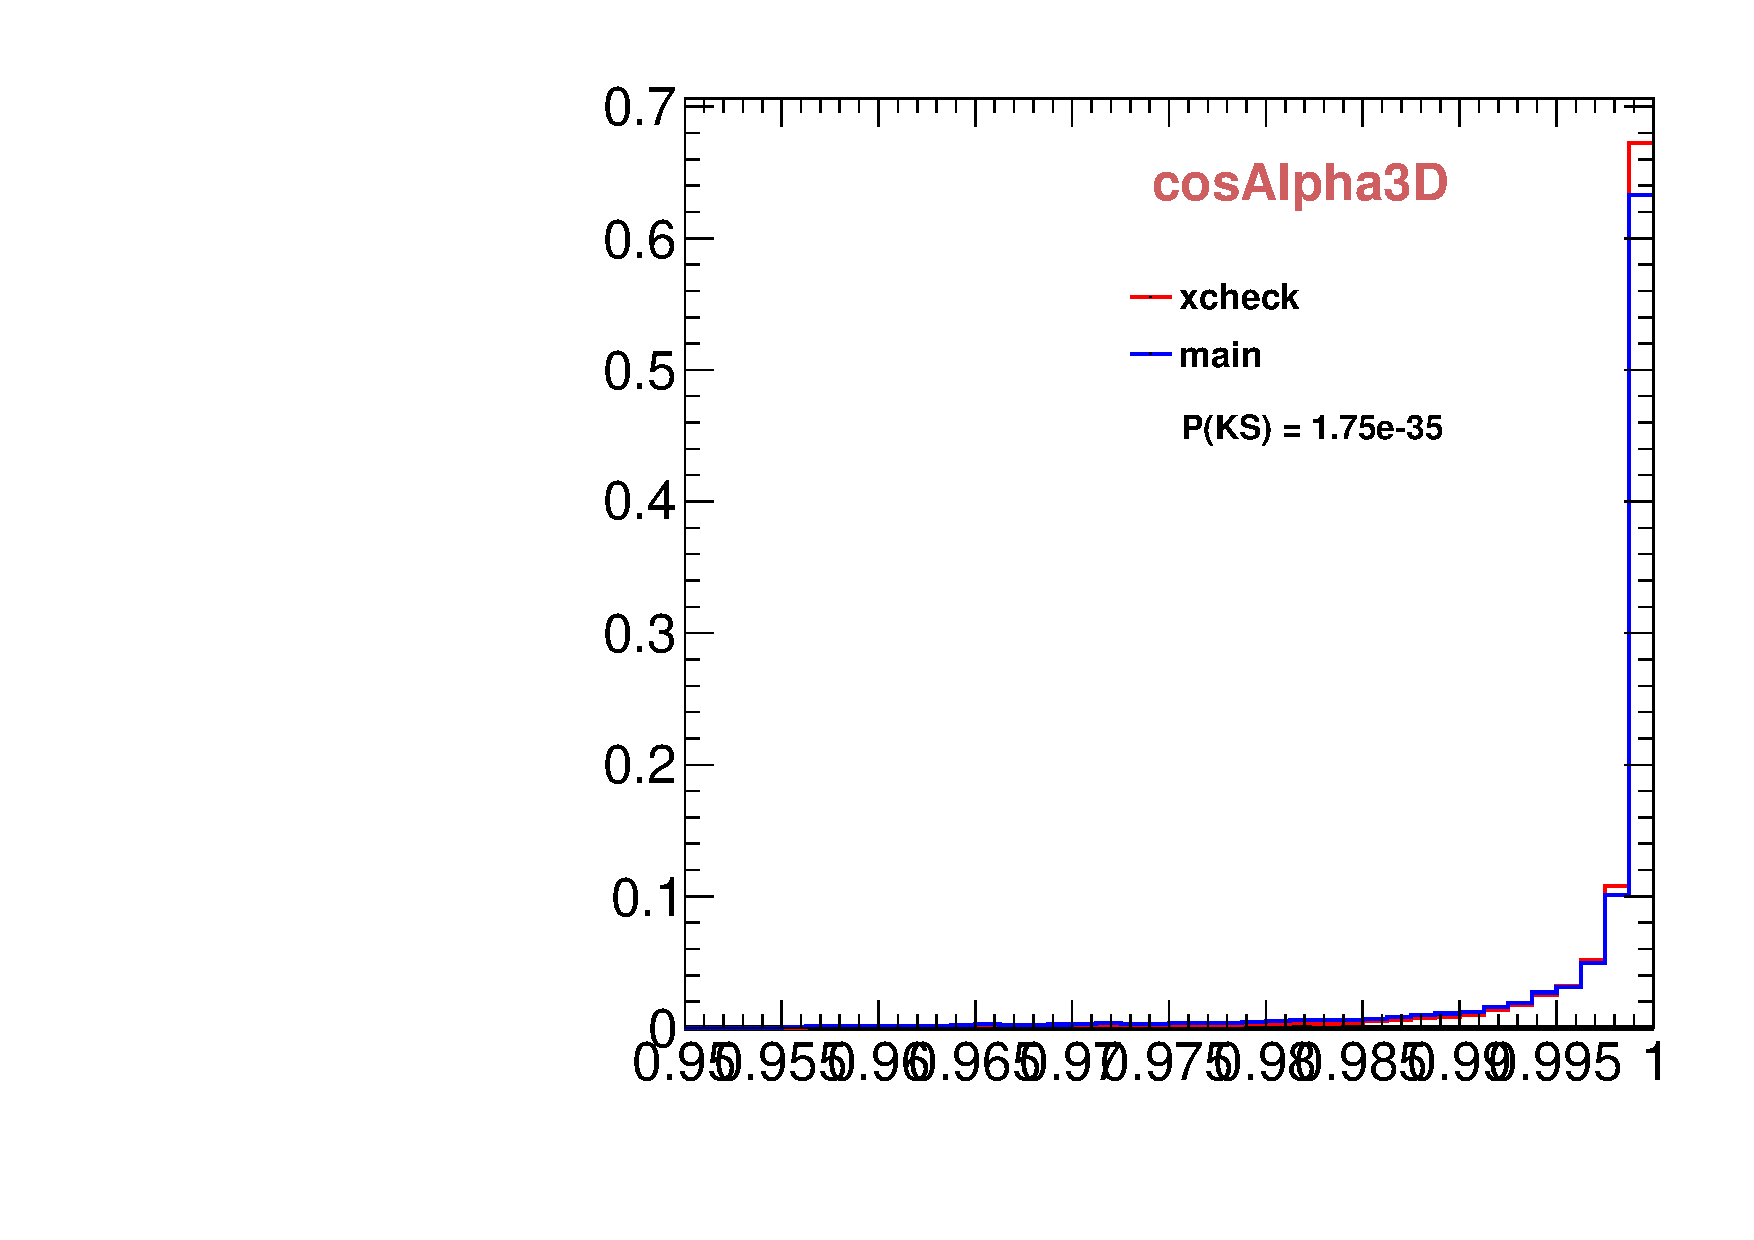
\includegraphics[width=0.3\textwidth]{Figures/VariablesComparison/MC_barrel_figs/cosa}
  %\label{fig:MC_barrel_cosa}
  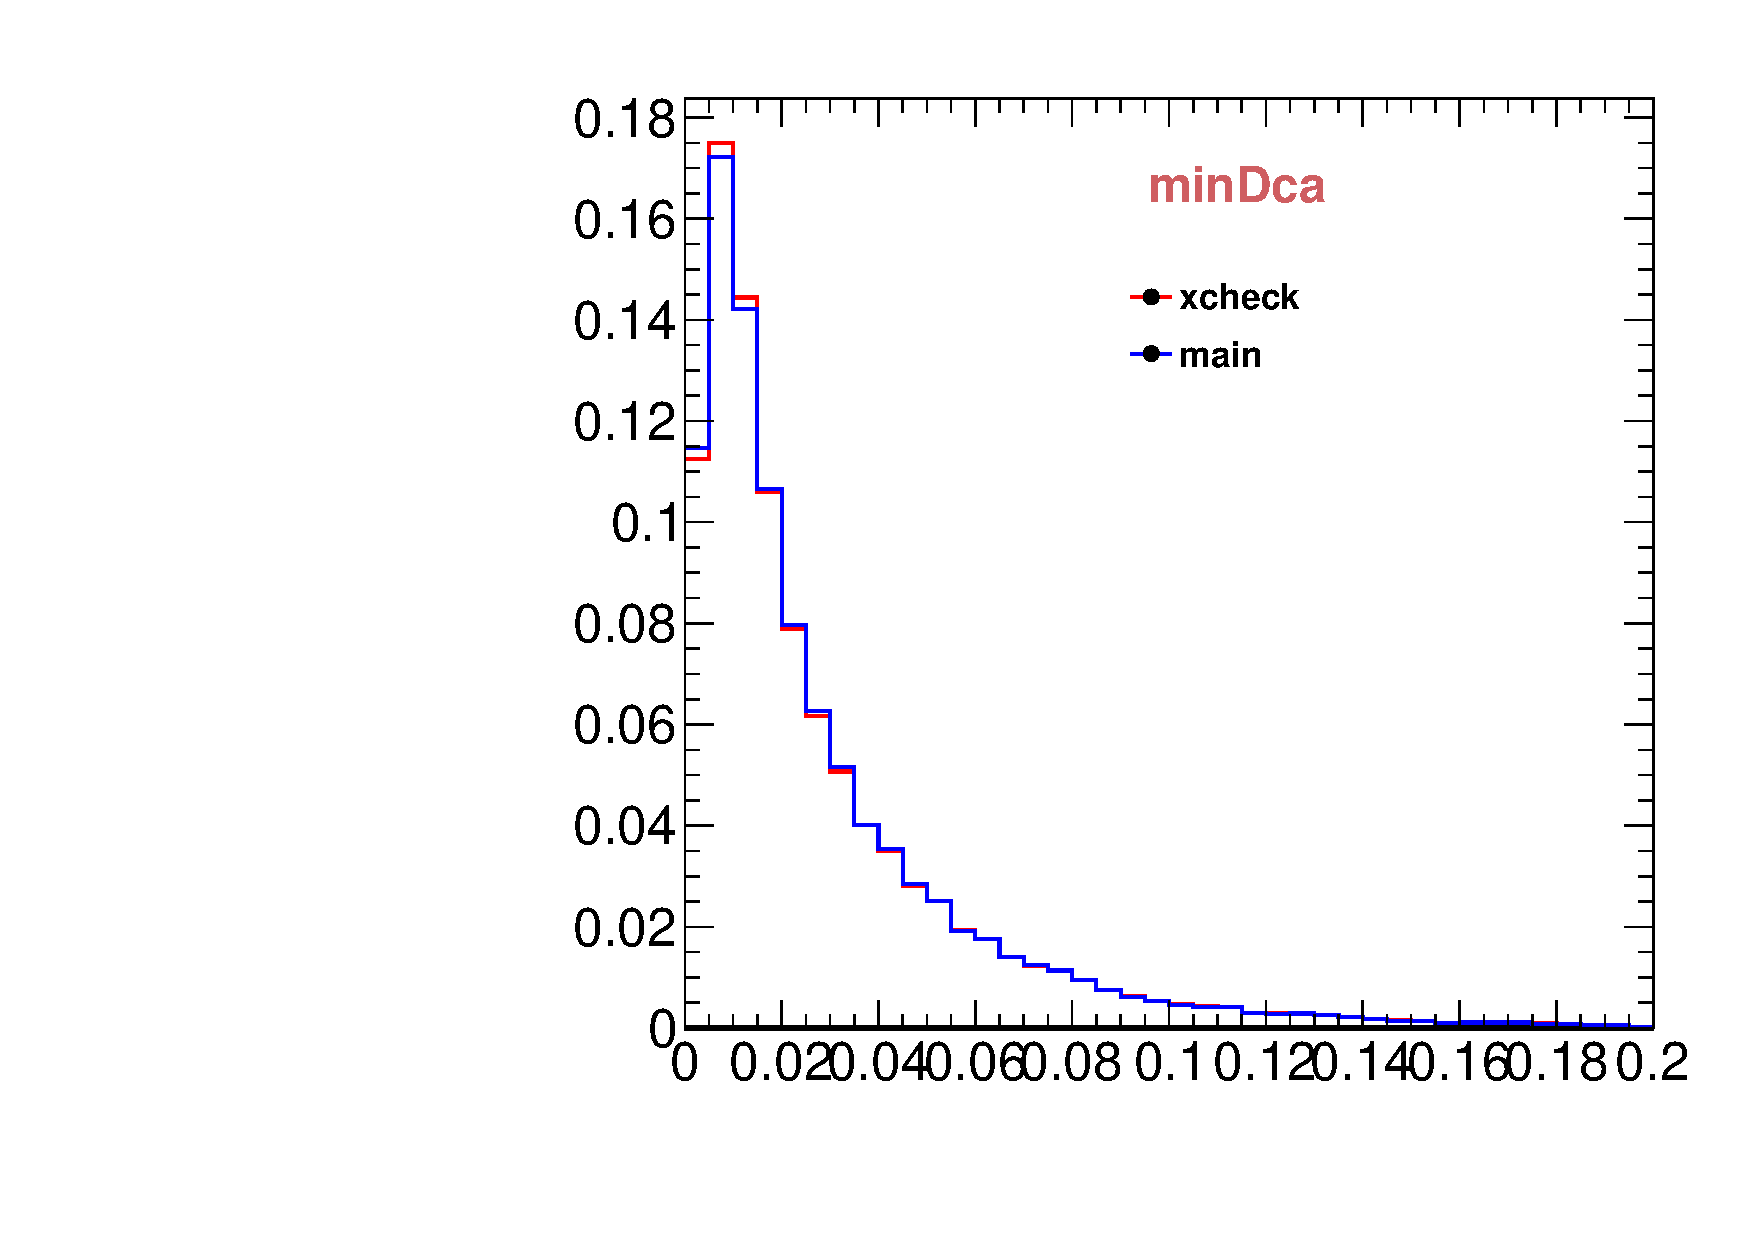
\includegraphics[width=0.3\textwidth]{Figures/VariablesComparison/MC_barrel_figs/docatrk}
  %\label{fig:MC_barrel_docatrk}
  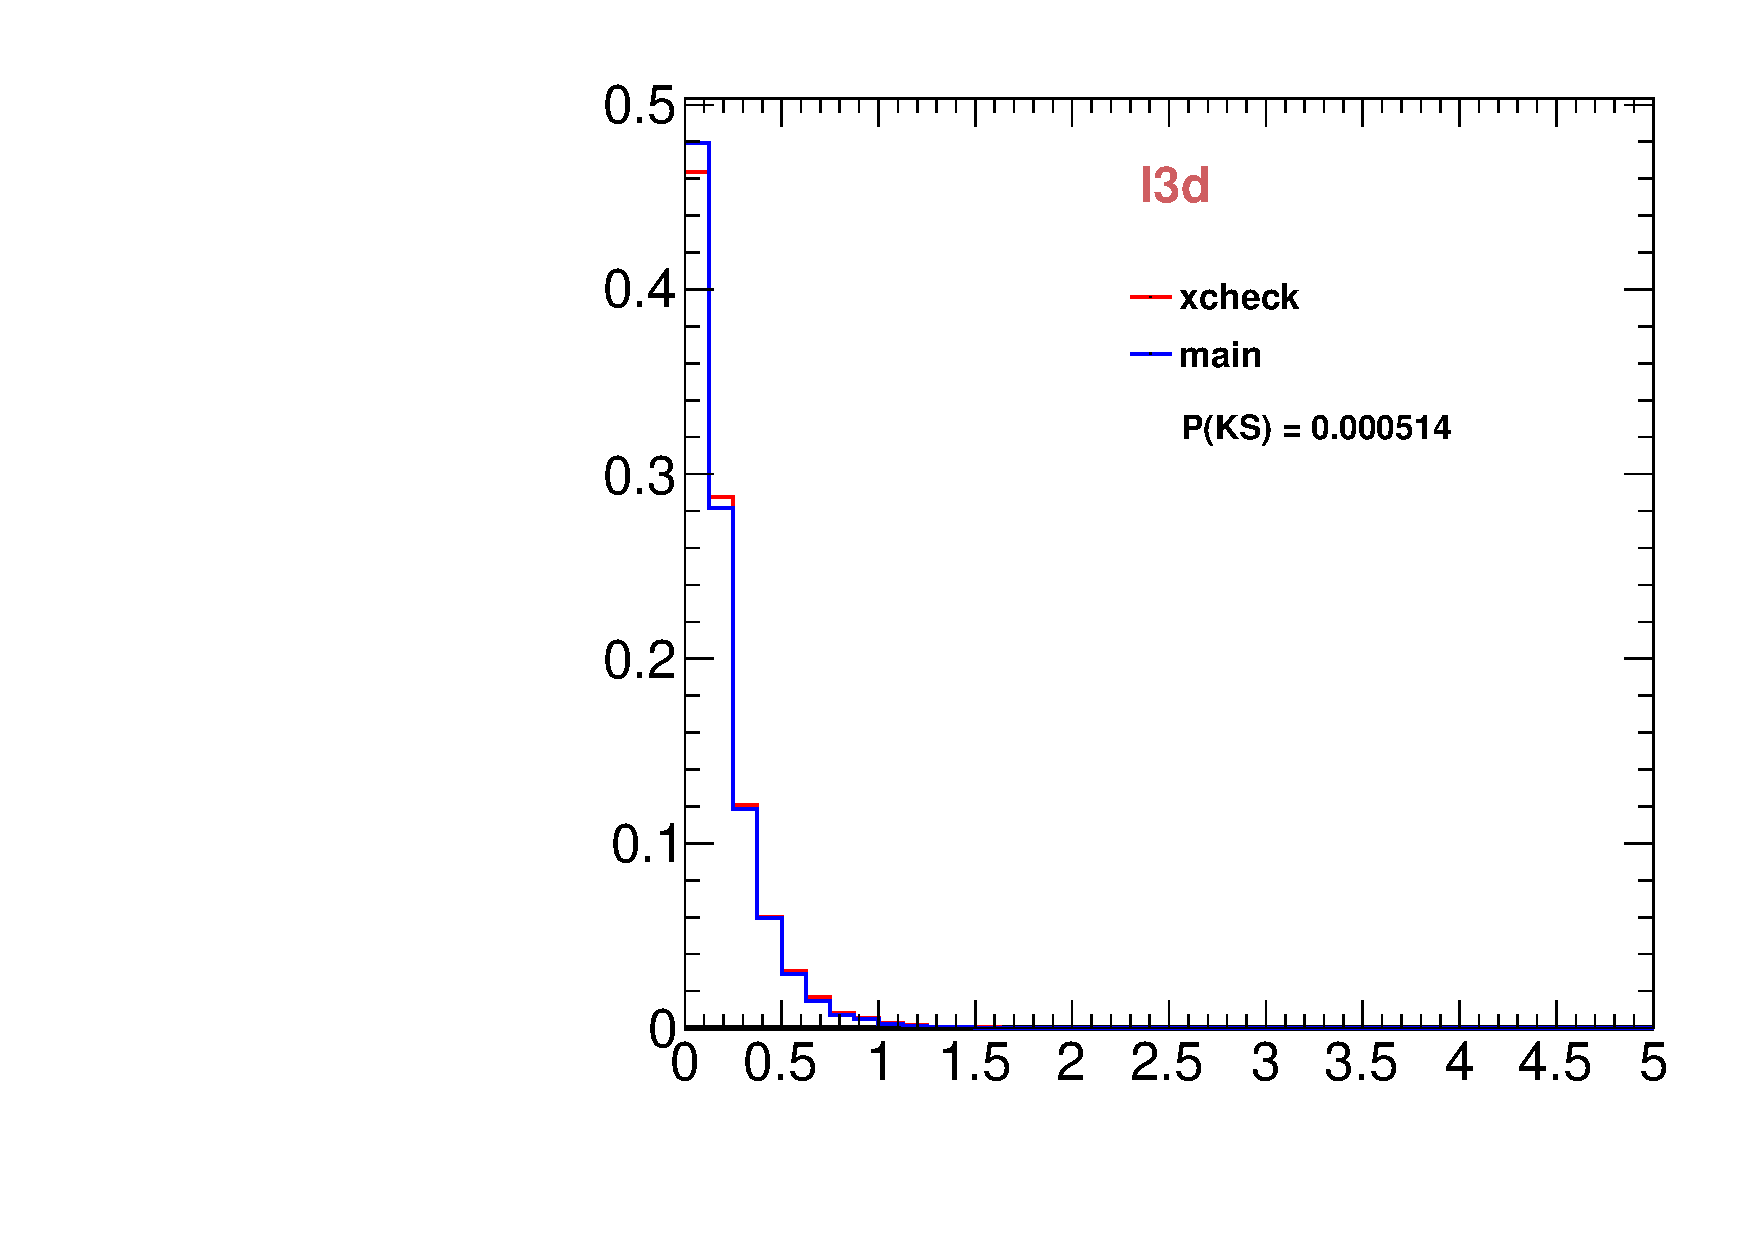
\includegraphics[width=0.3\textwidth]{Figures/VariablesComparison/MC_barrel_figs/fl3d}
  %\label{fig:MC_barrel_fl3d}
  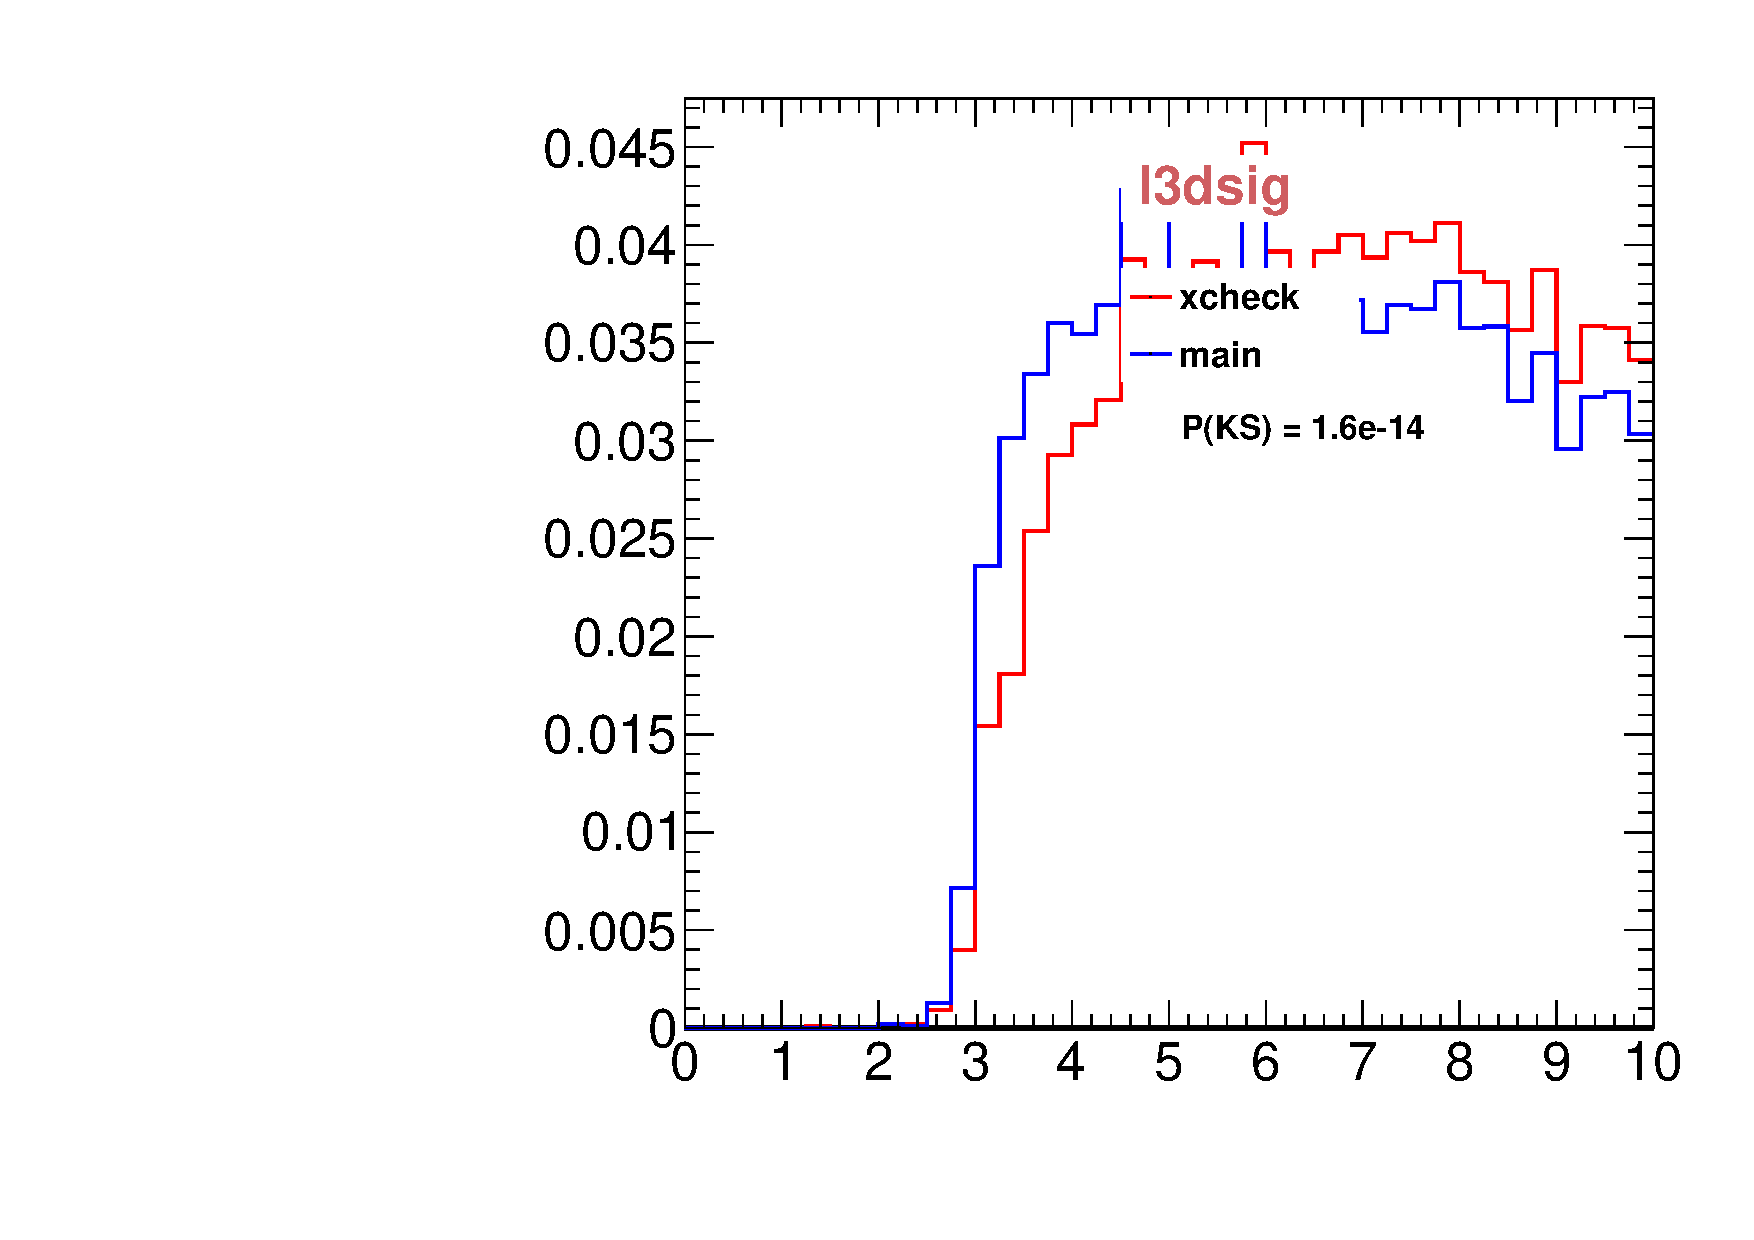
\includegraphics[width=0.3\textwidth]{Figures/VariablesComparison/MC_barrel_figs/fls3d}
  %\label{fig:MC_barrel_fls3d}
  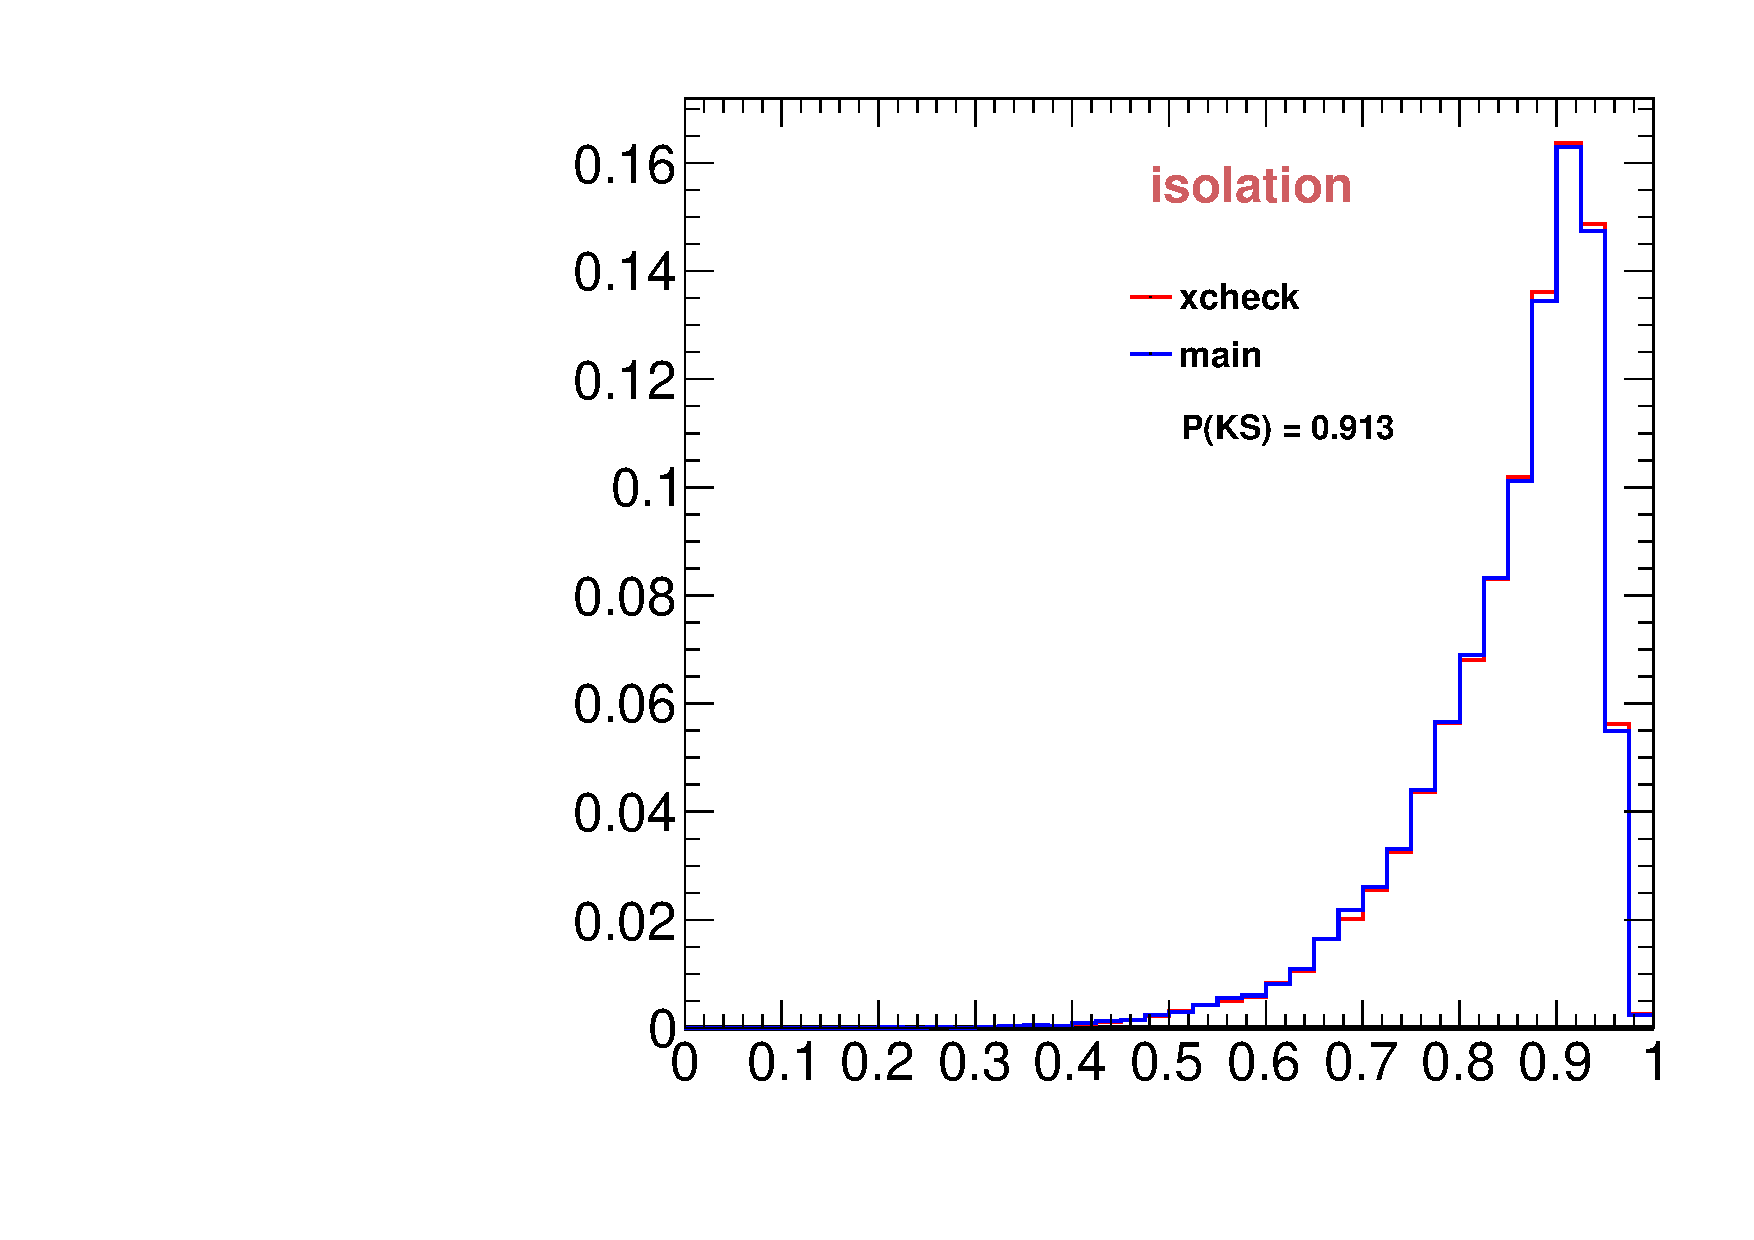
\includegraphics[width=0.3\textwidth]{Figures/VariablesComparison/MC_barrel_figs/iso}
  %\label{fig:MC_barrel_iso}
  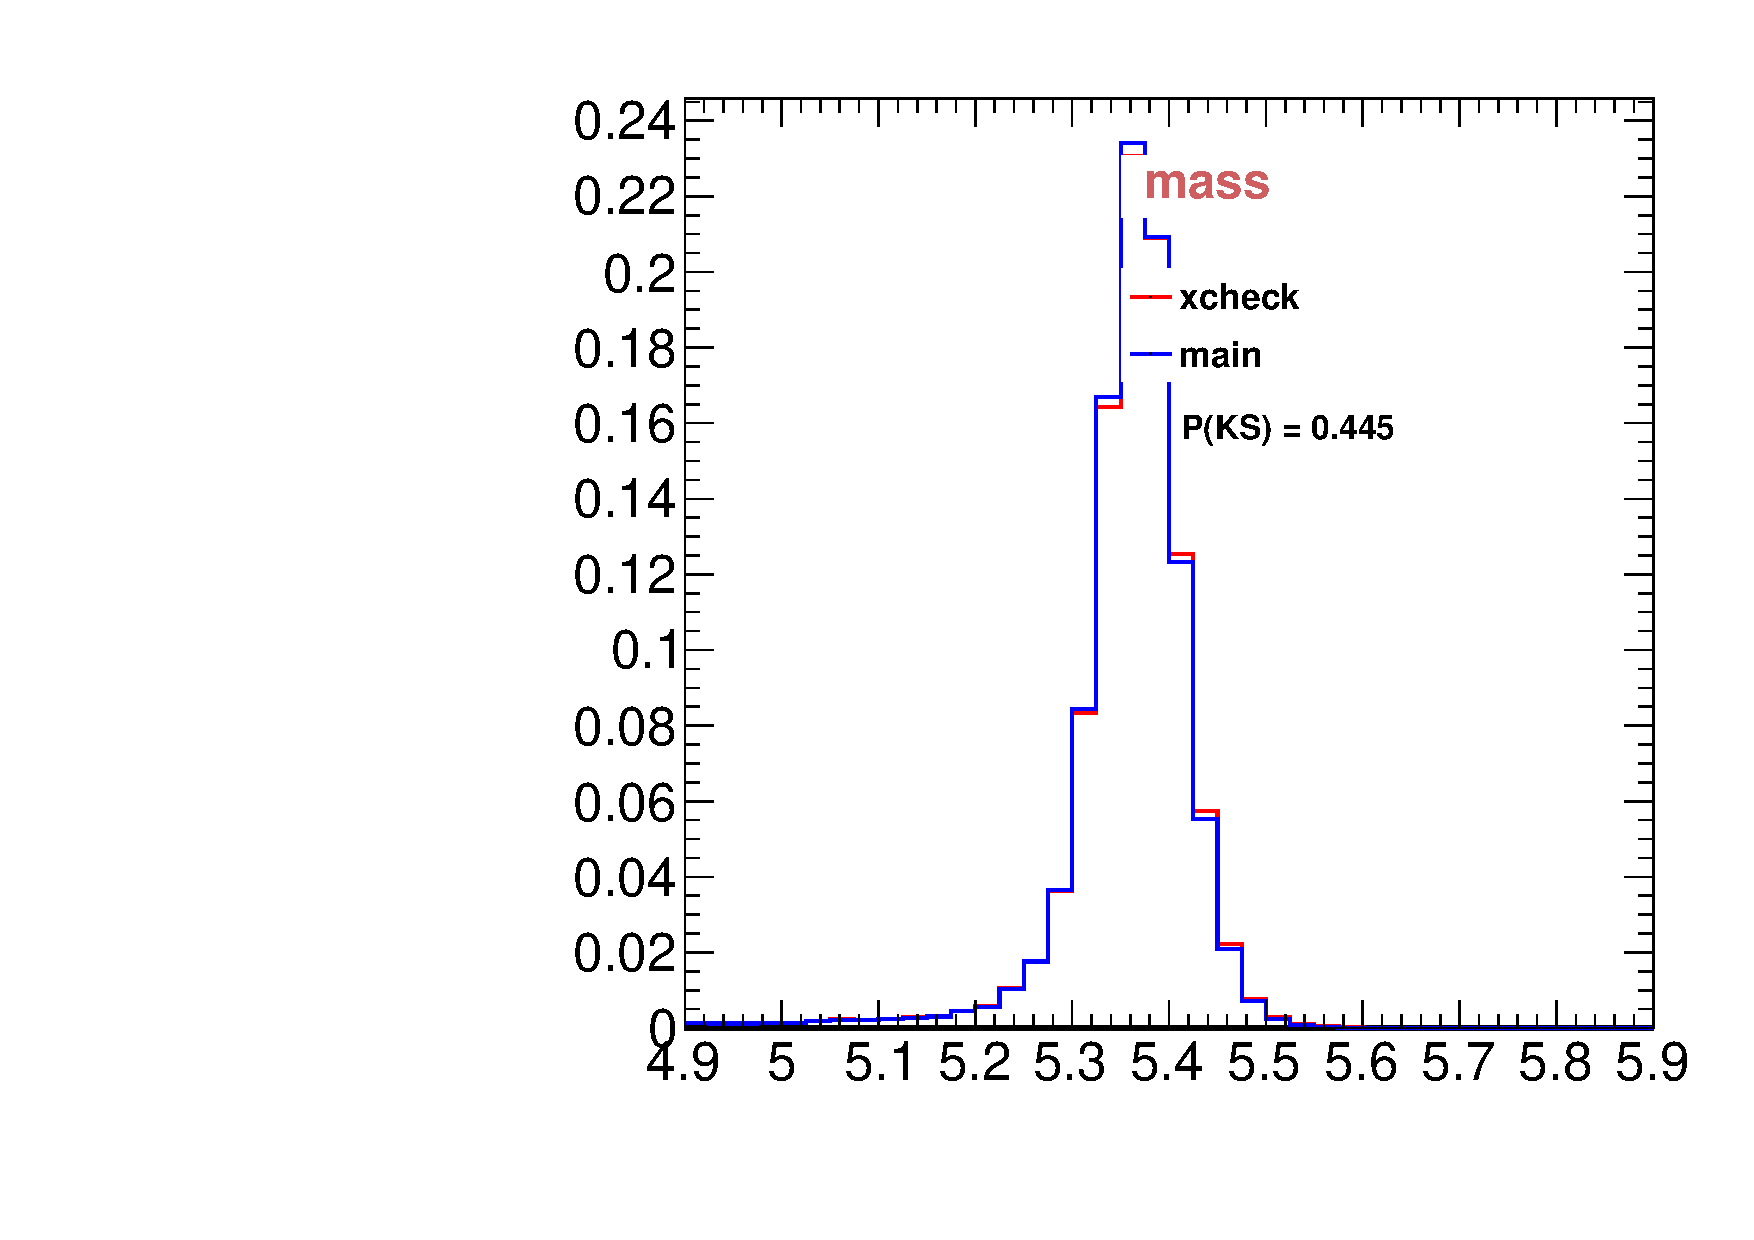
\includegraphics[width=0.3\textwidth]{Figures/VariablesComparison/MC_barrel_figs/m}
  %\label{fig:MC_barrel_m}
  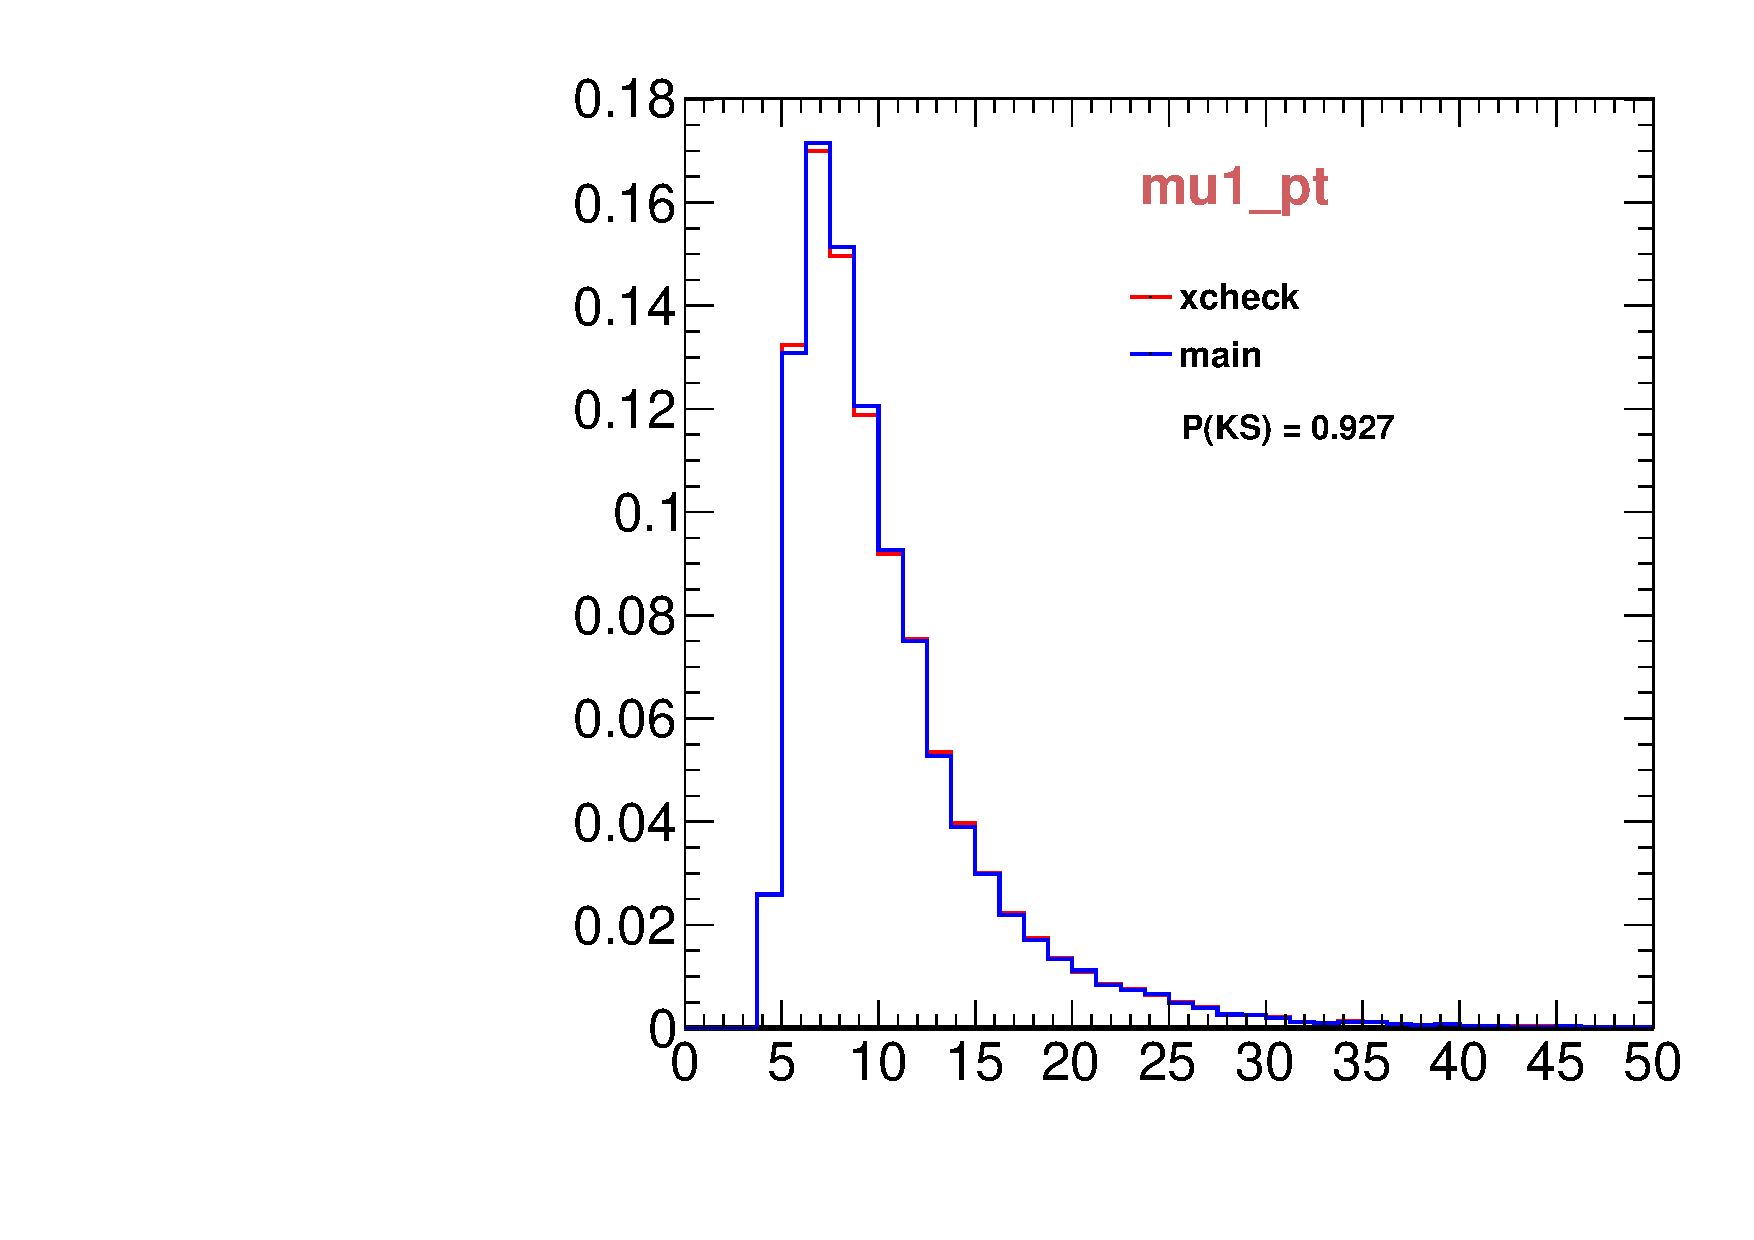
\includegraphics[width=0.3\textwidth]{Figures/VariablesComparison/MC_barrel_figs/m1pt}
  %\label{fig:MC_barrel_m1pt}
  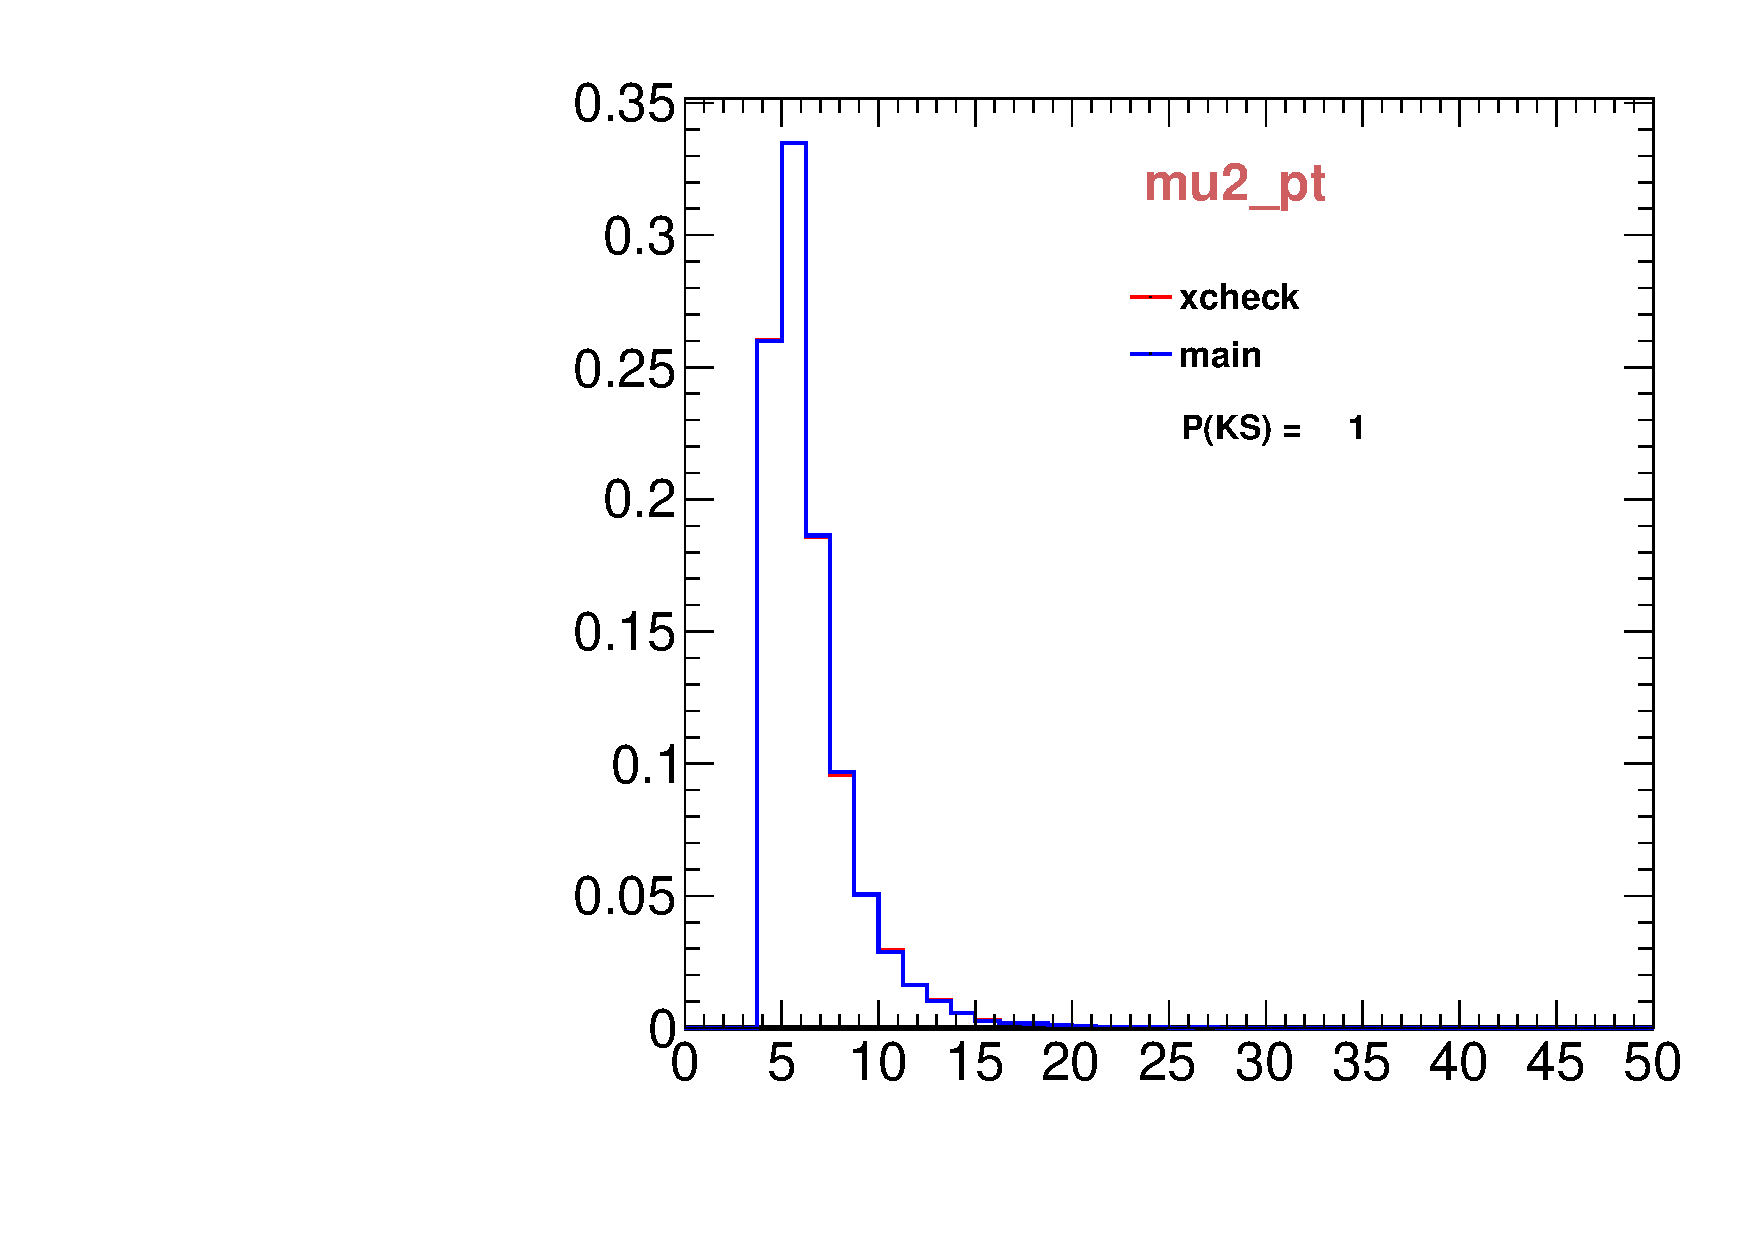
\includegraphics[width=0.3\textwidth]{Figures/VariablesComparison/MC_barrel_figs/m2pt}
  %\label{fig:MC_barrel_m2pt}
  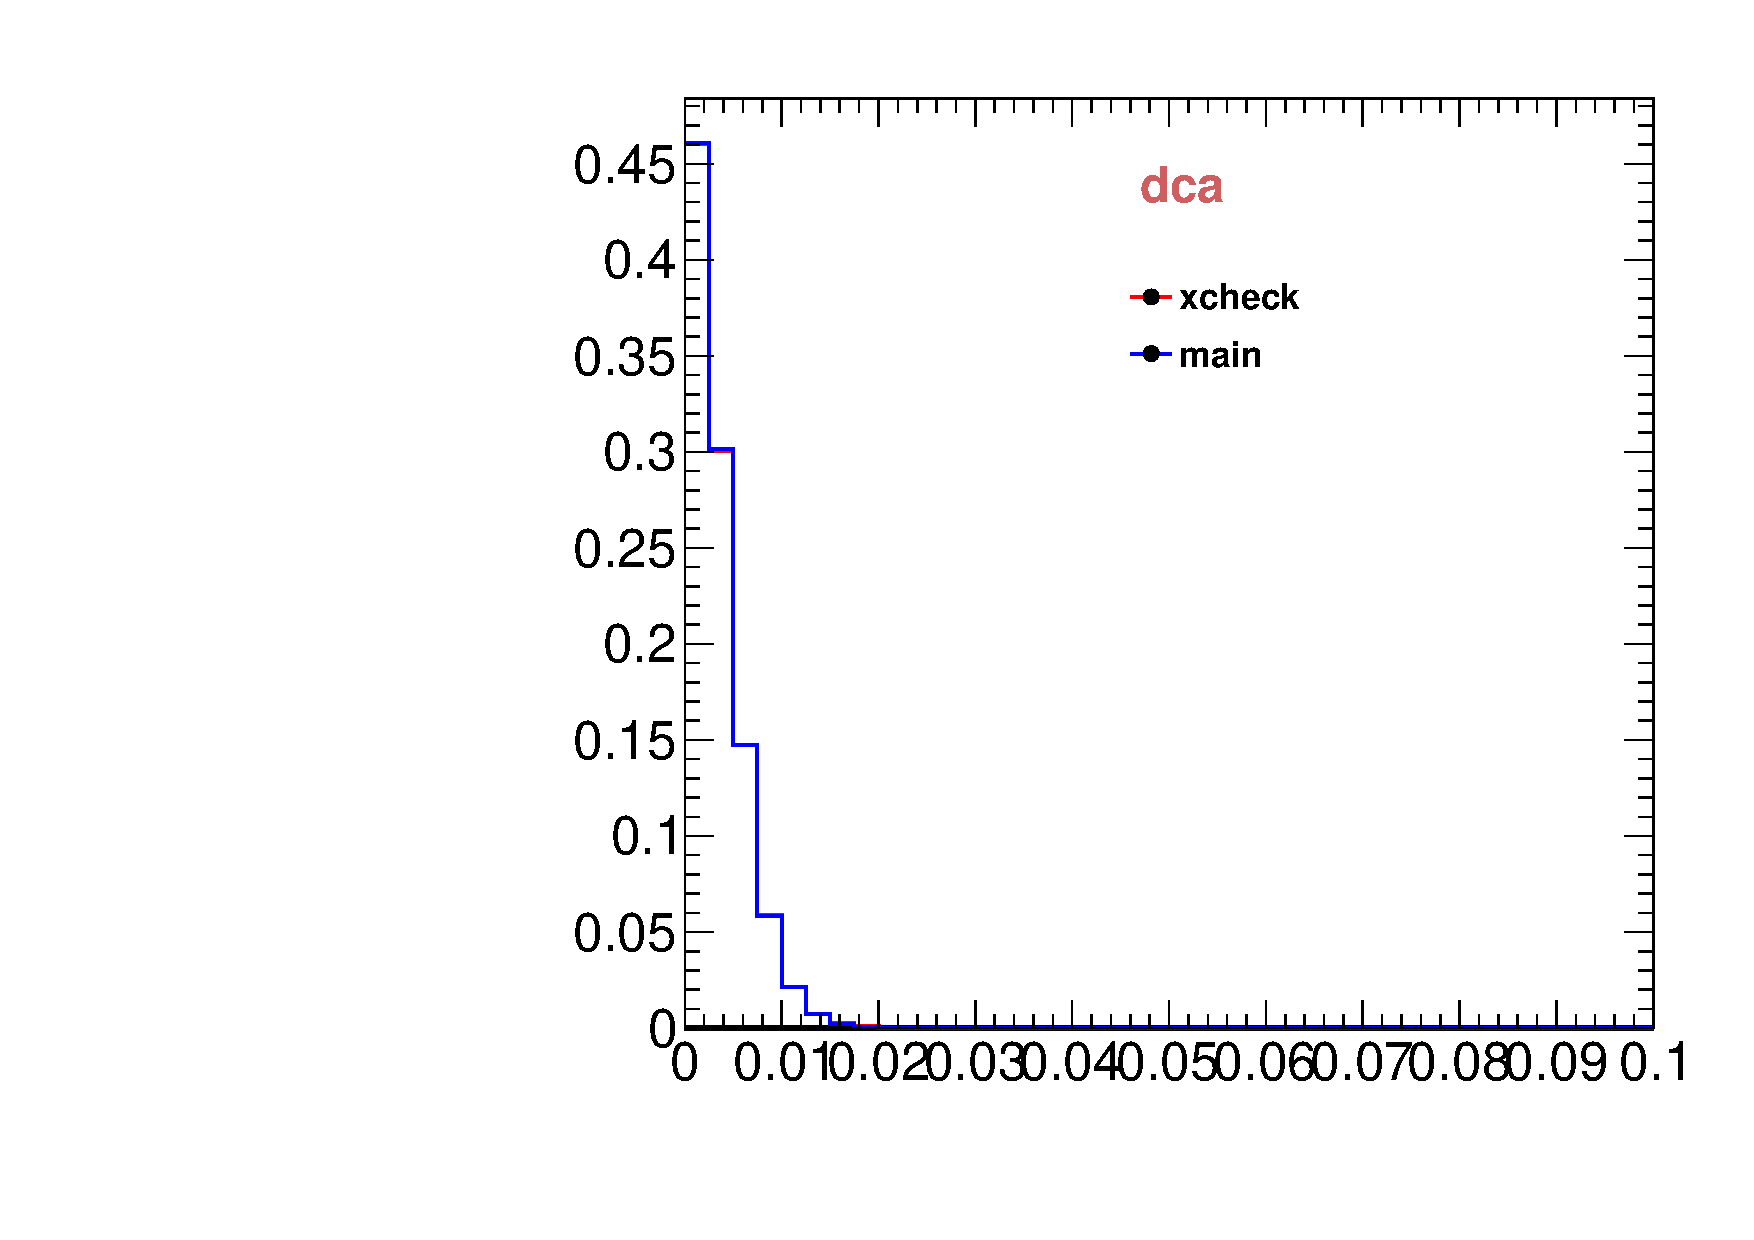
\includegraphics[width=0.3\textwidth]{Figures/VariablesComparison/MC_barrel_figs/maxdoca}
  %\label{fig:MC_barrel_maxdoca}
  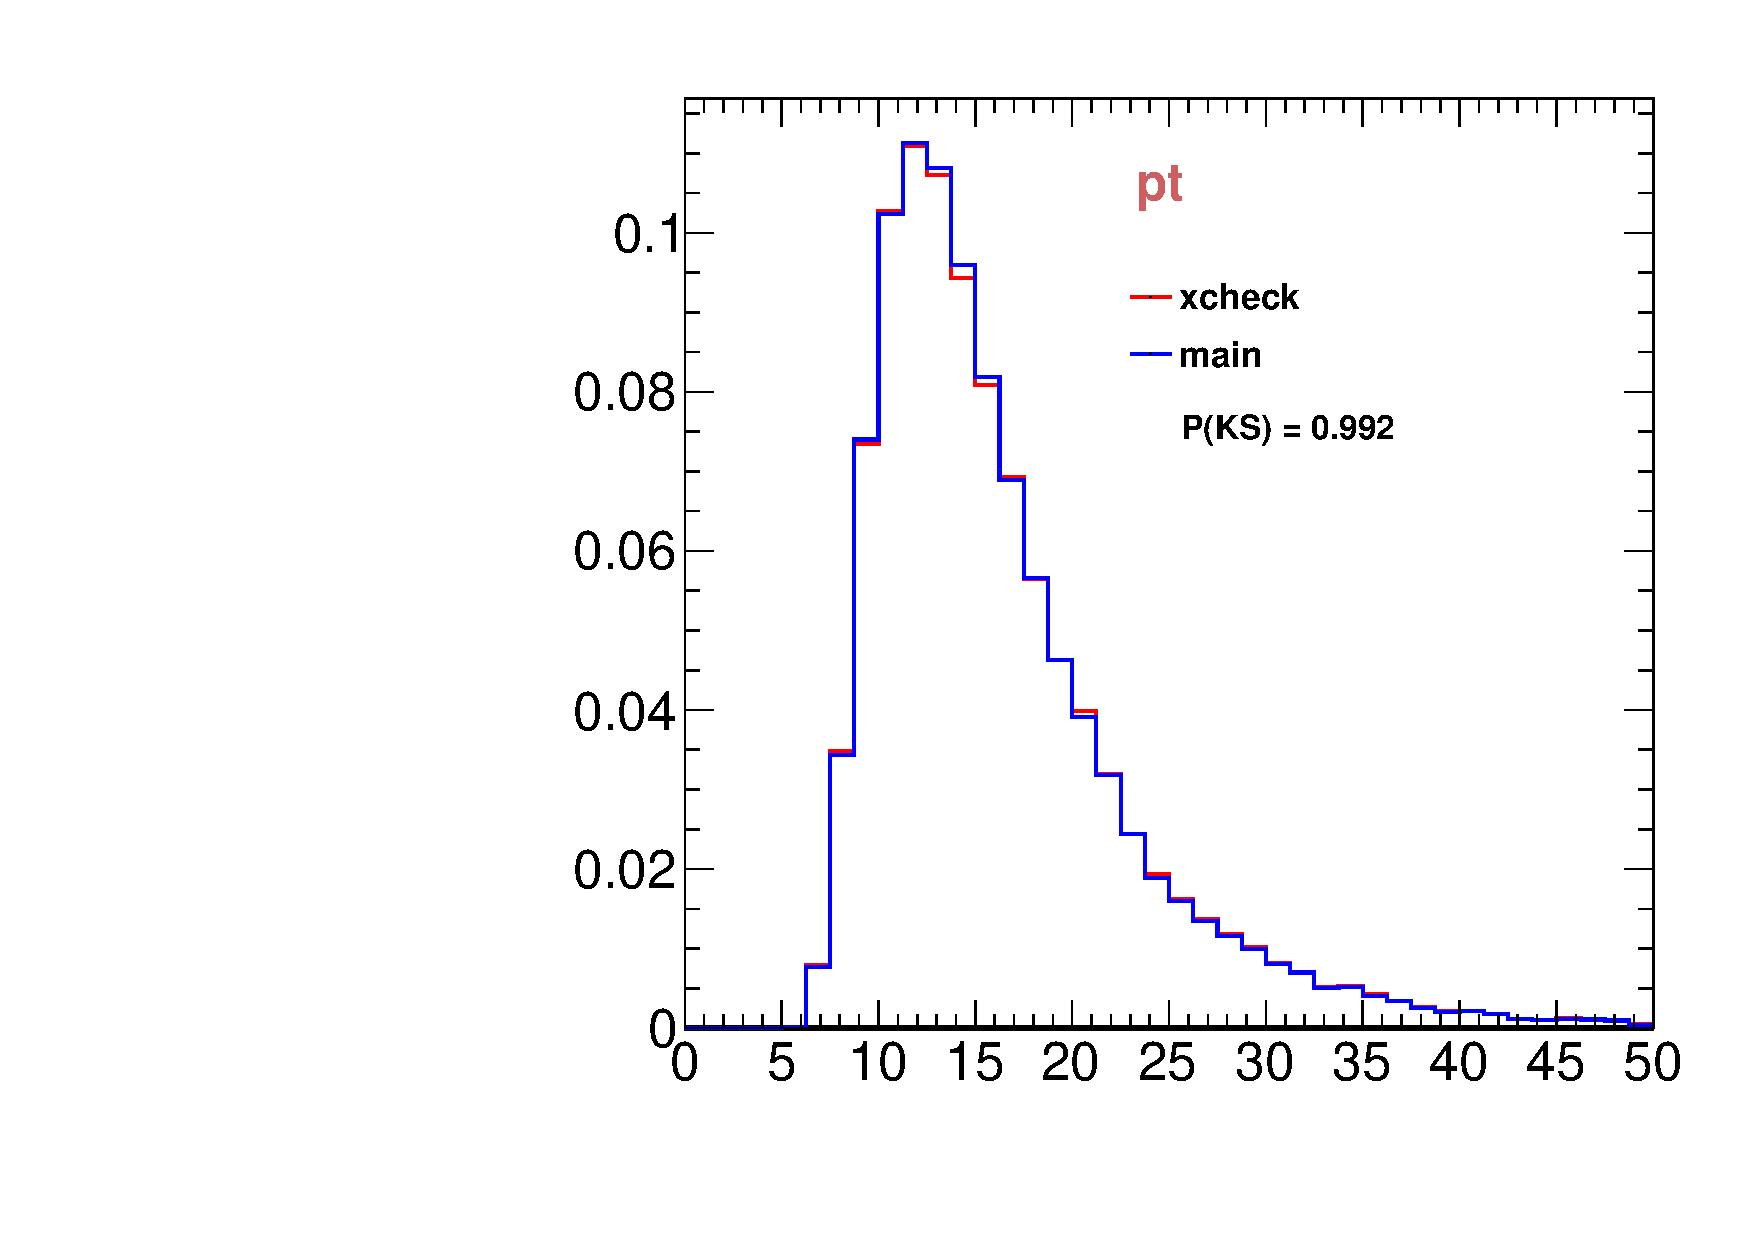
\includegraphics[width=0.3\textwidth]{Figures/VariablesComparison/MC_barrel_figs/pt}
  %\label{fig:MC_barrel_pt}
  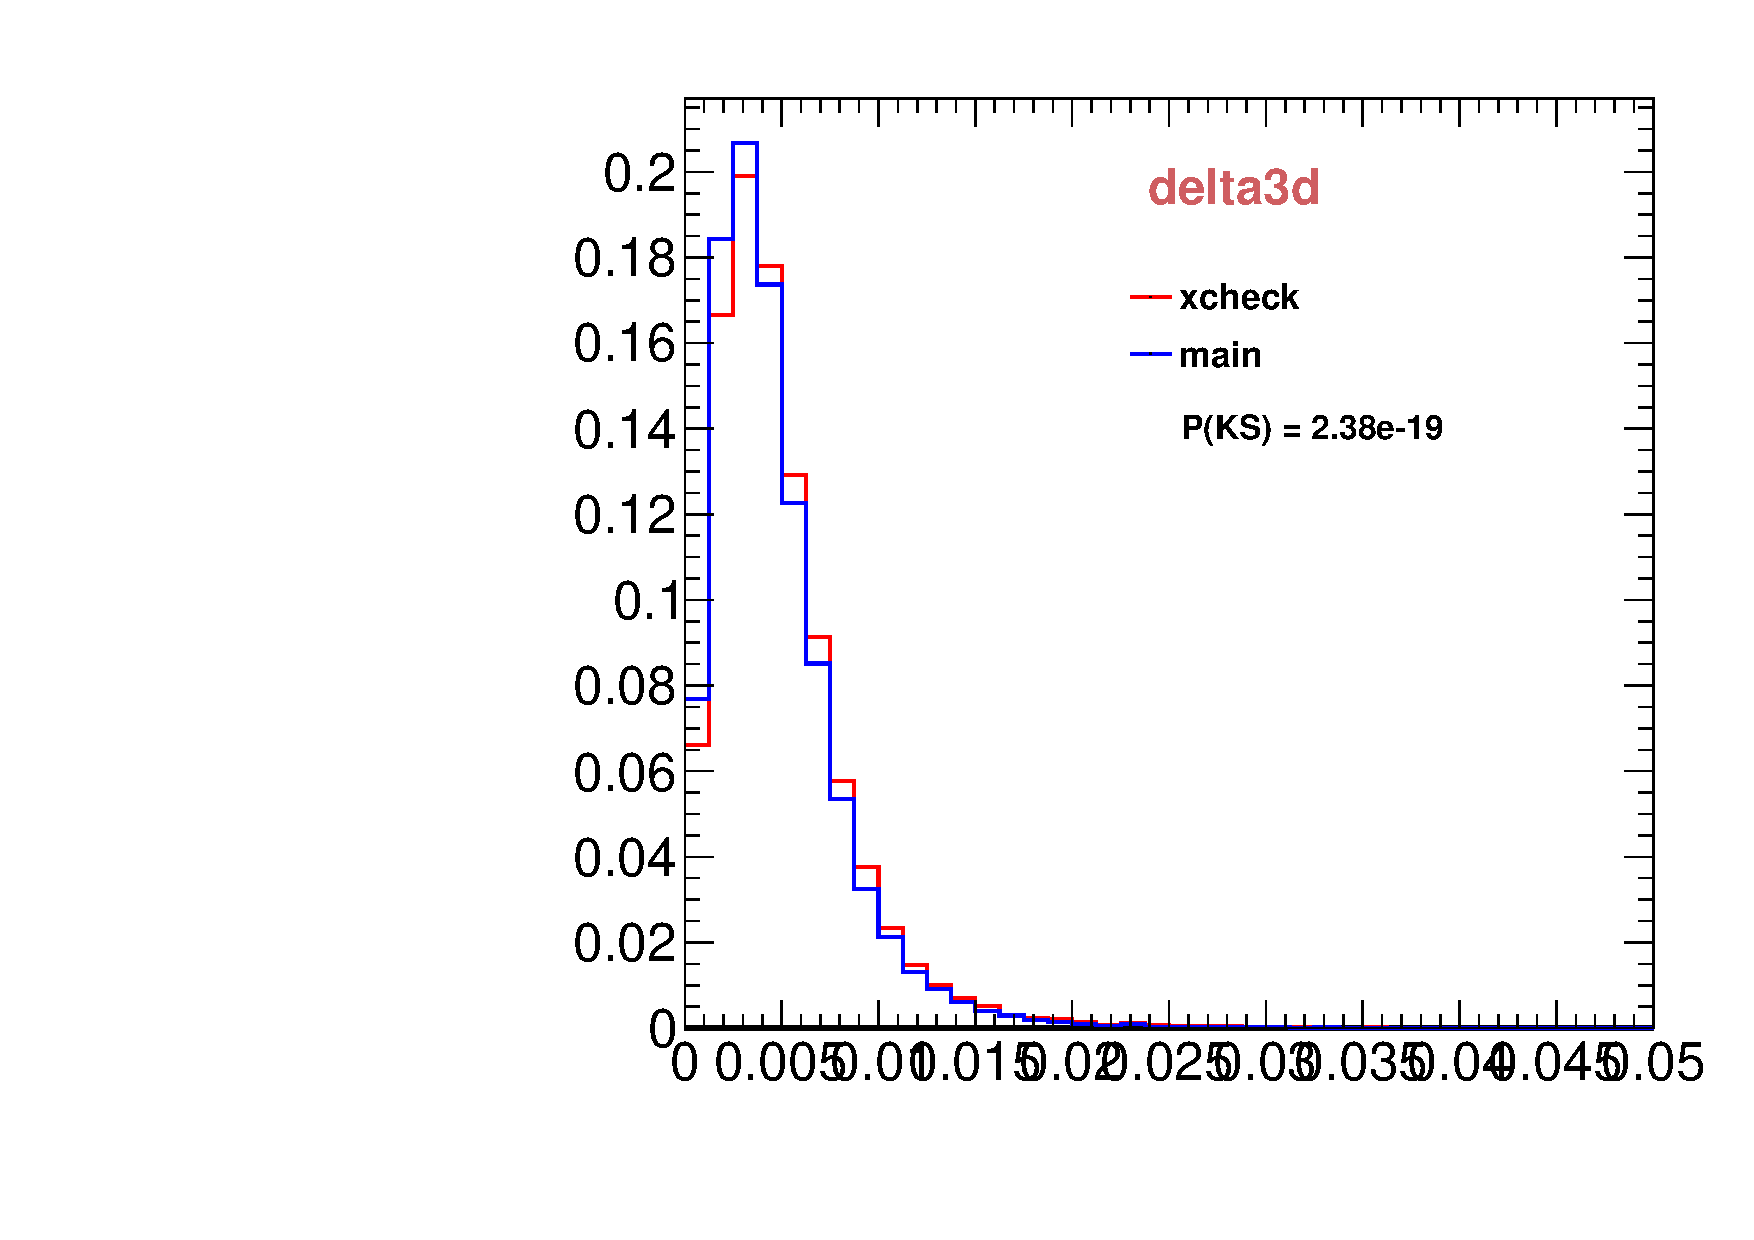
\includegraphics[width=0.3\textwidth]{Figures/VariablesComparison/MC_barrel_figs/pvip}
  %\label{fig:MC_barrel_pvip}
  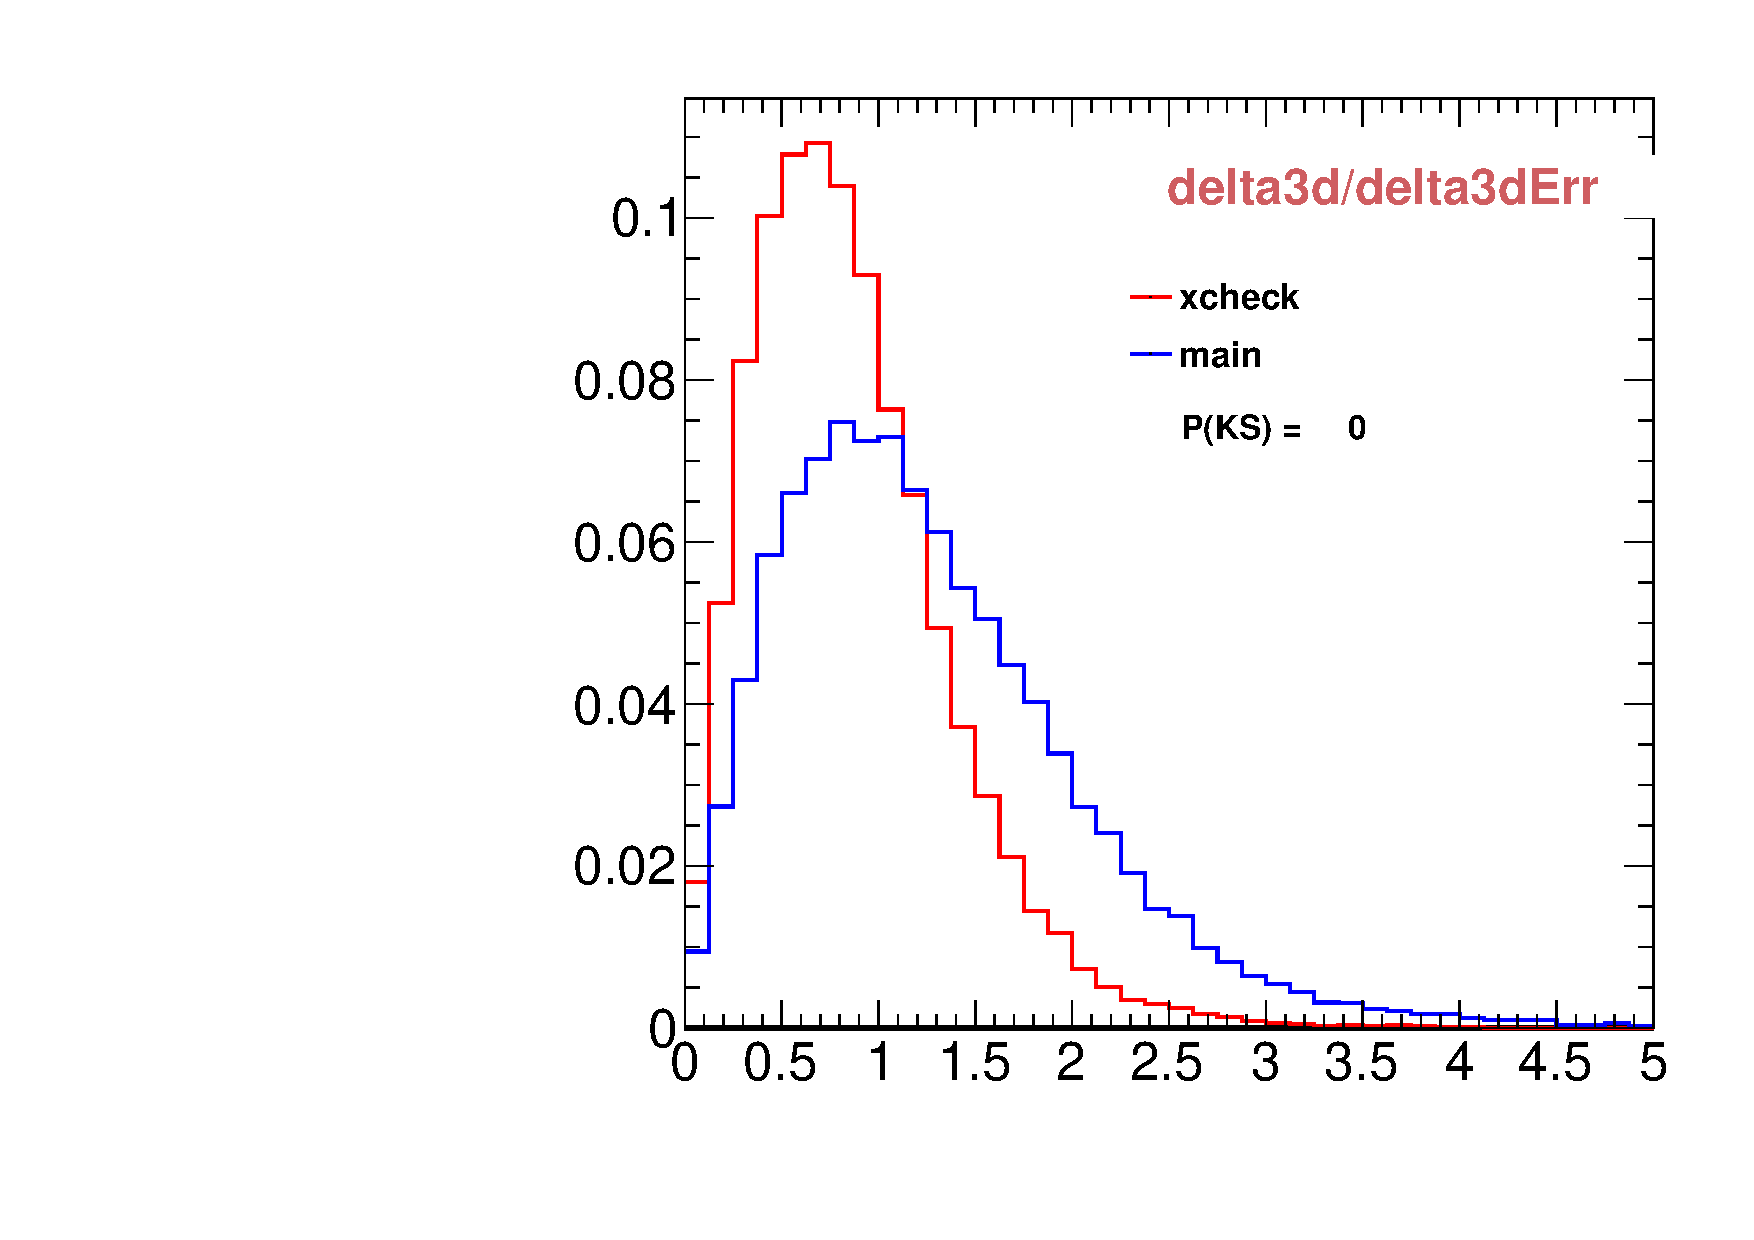
\includegraphics[width=0.3\textwidth]{Figures/VariablesComparison/MC_barrel_figs/pvips}
  %\label{fig:MC_barrel_pvips}
  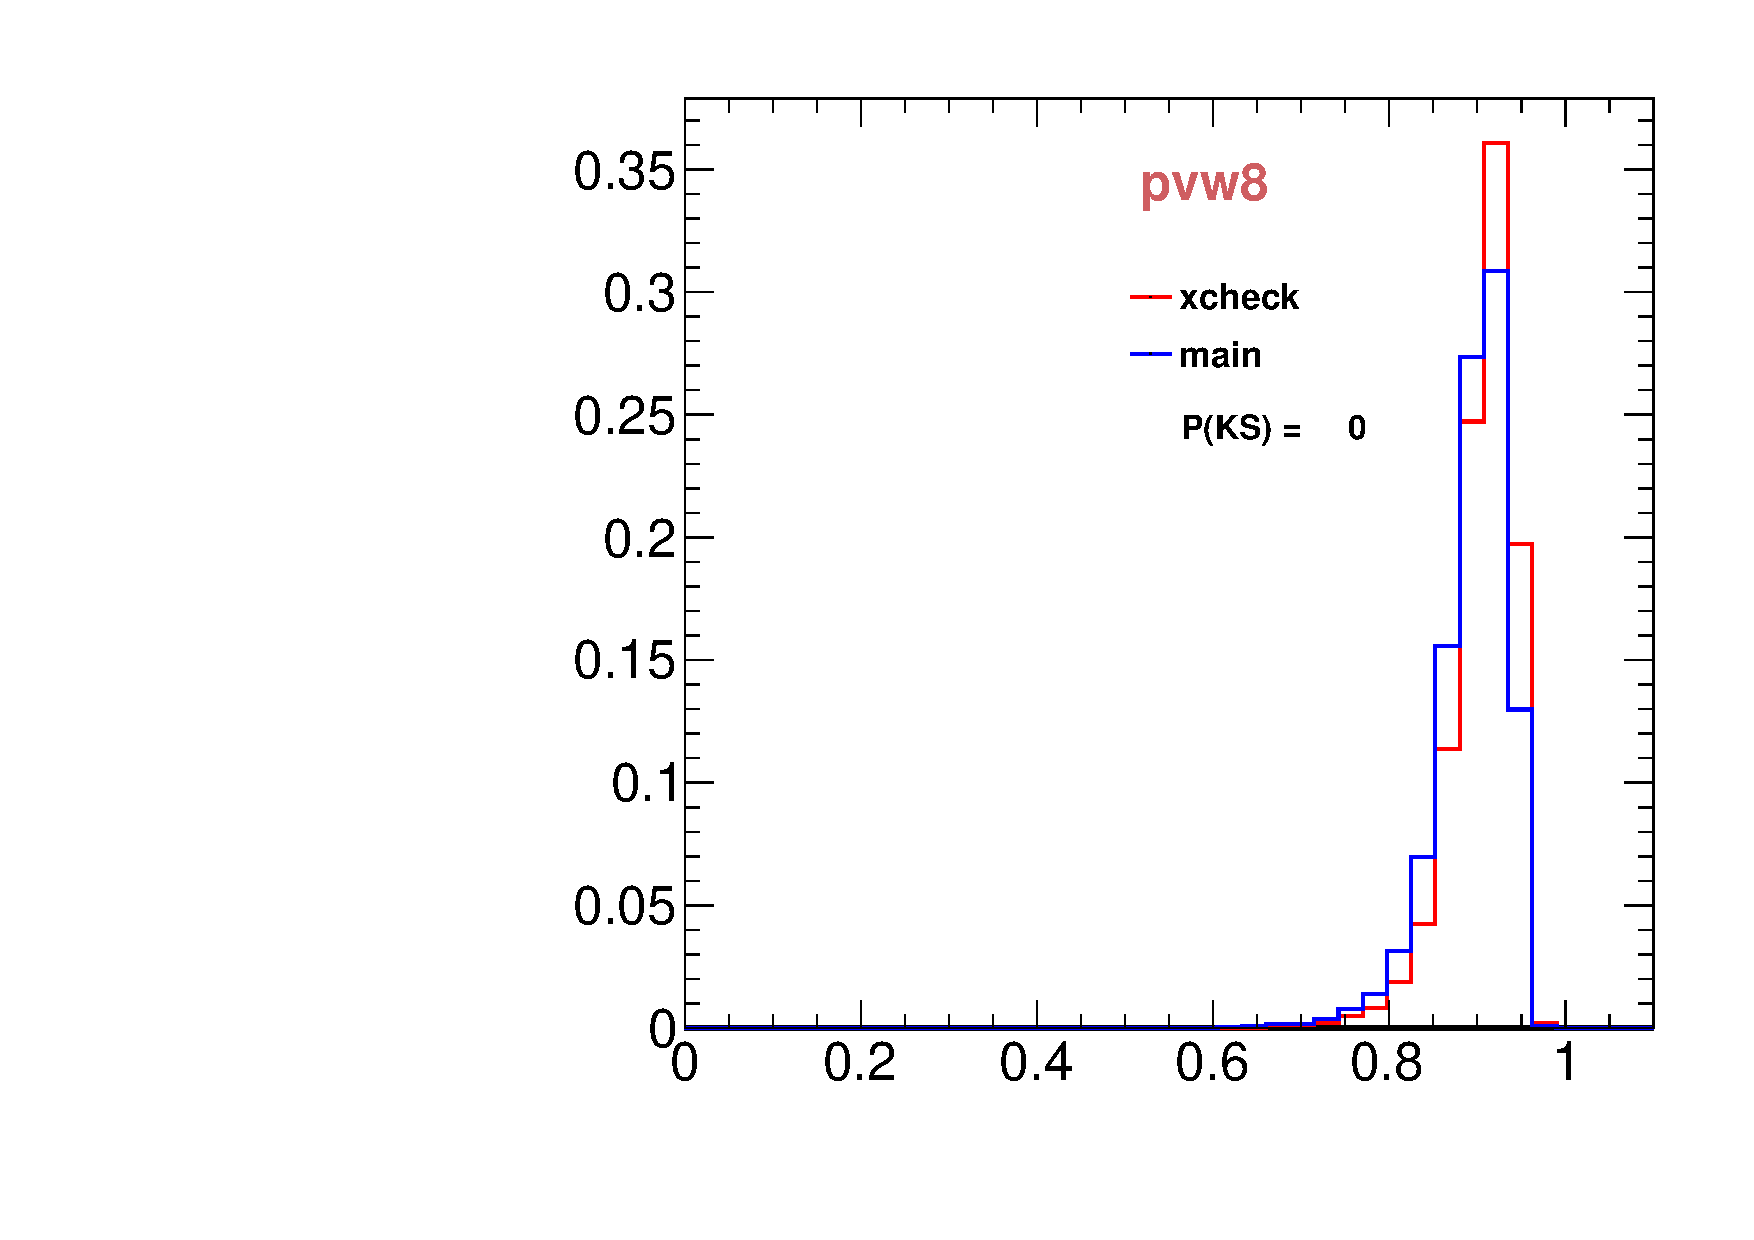
\includegraphics[width=0.3\textwidth]{Figures/VariablesComparison/MC_barrel_figs/pvw8}
  %\label{fig:MC_barrel_pvw8}
  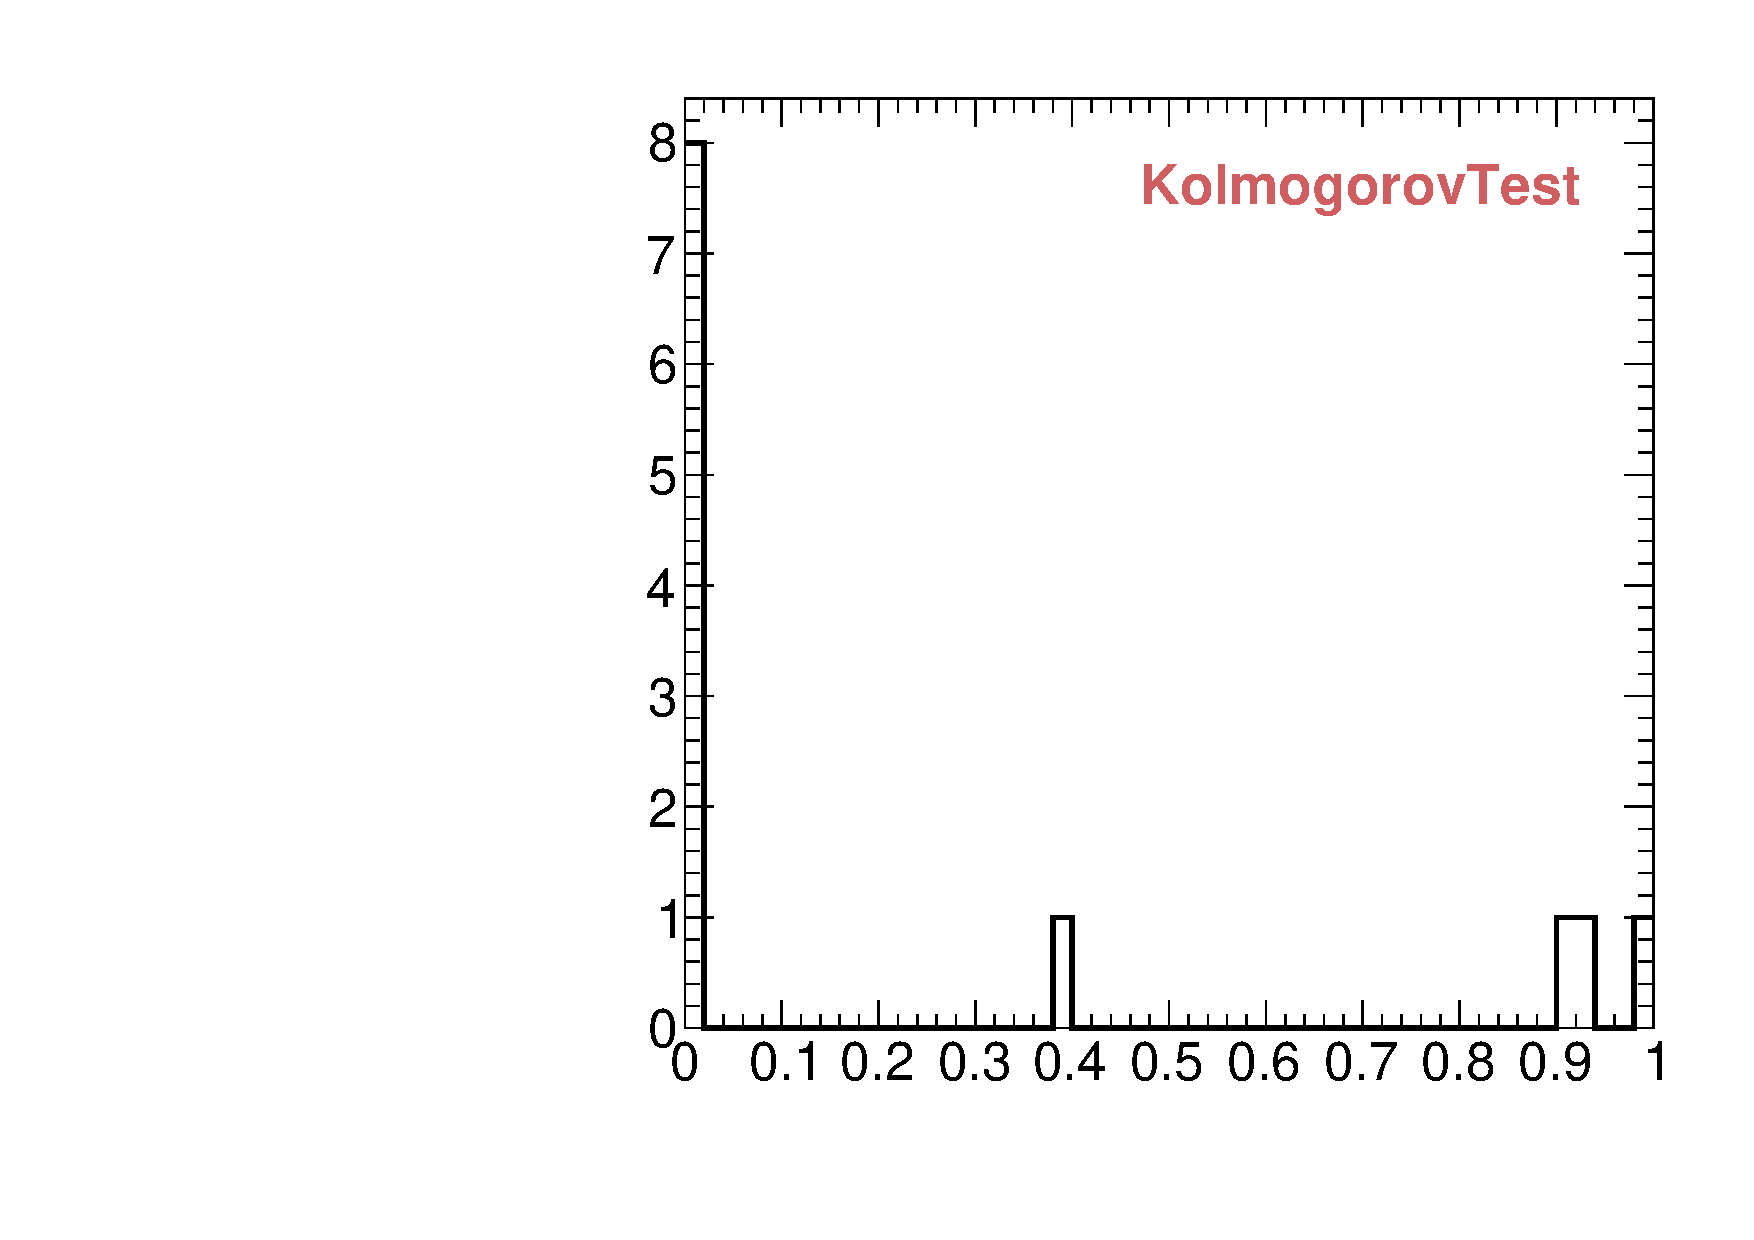
\includegraphics[width=0.3\textwidth]{Figures/VariablesComparison/MC_barrel_figs/KS}
  %\label{fig:MC_barrel_KS}
  \caption{Variable comparisons between the main analysis and the cross-check analysis. Part I: MC barrel.}
  \label{fig:MC_barrel_figs}
\end{figure}

\begin{figure}
  \centering
  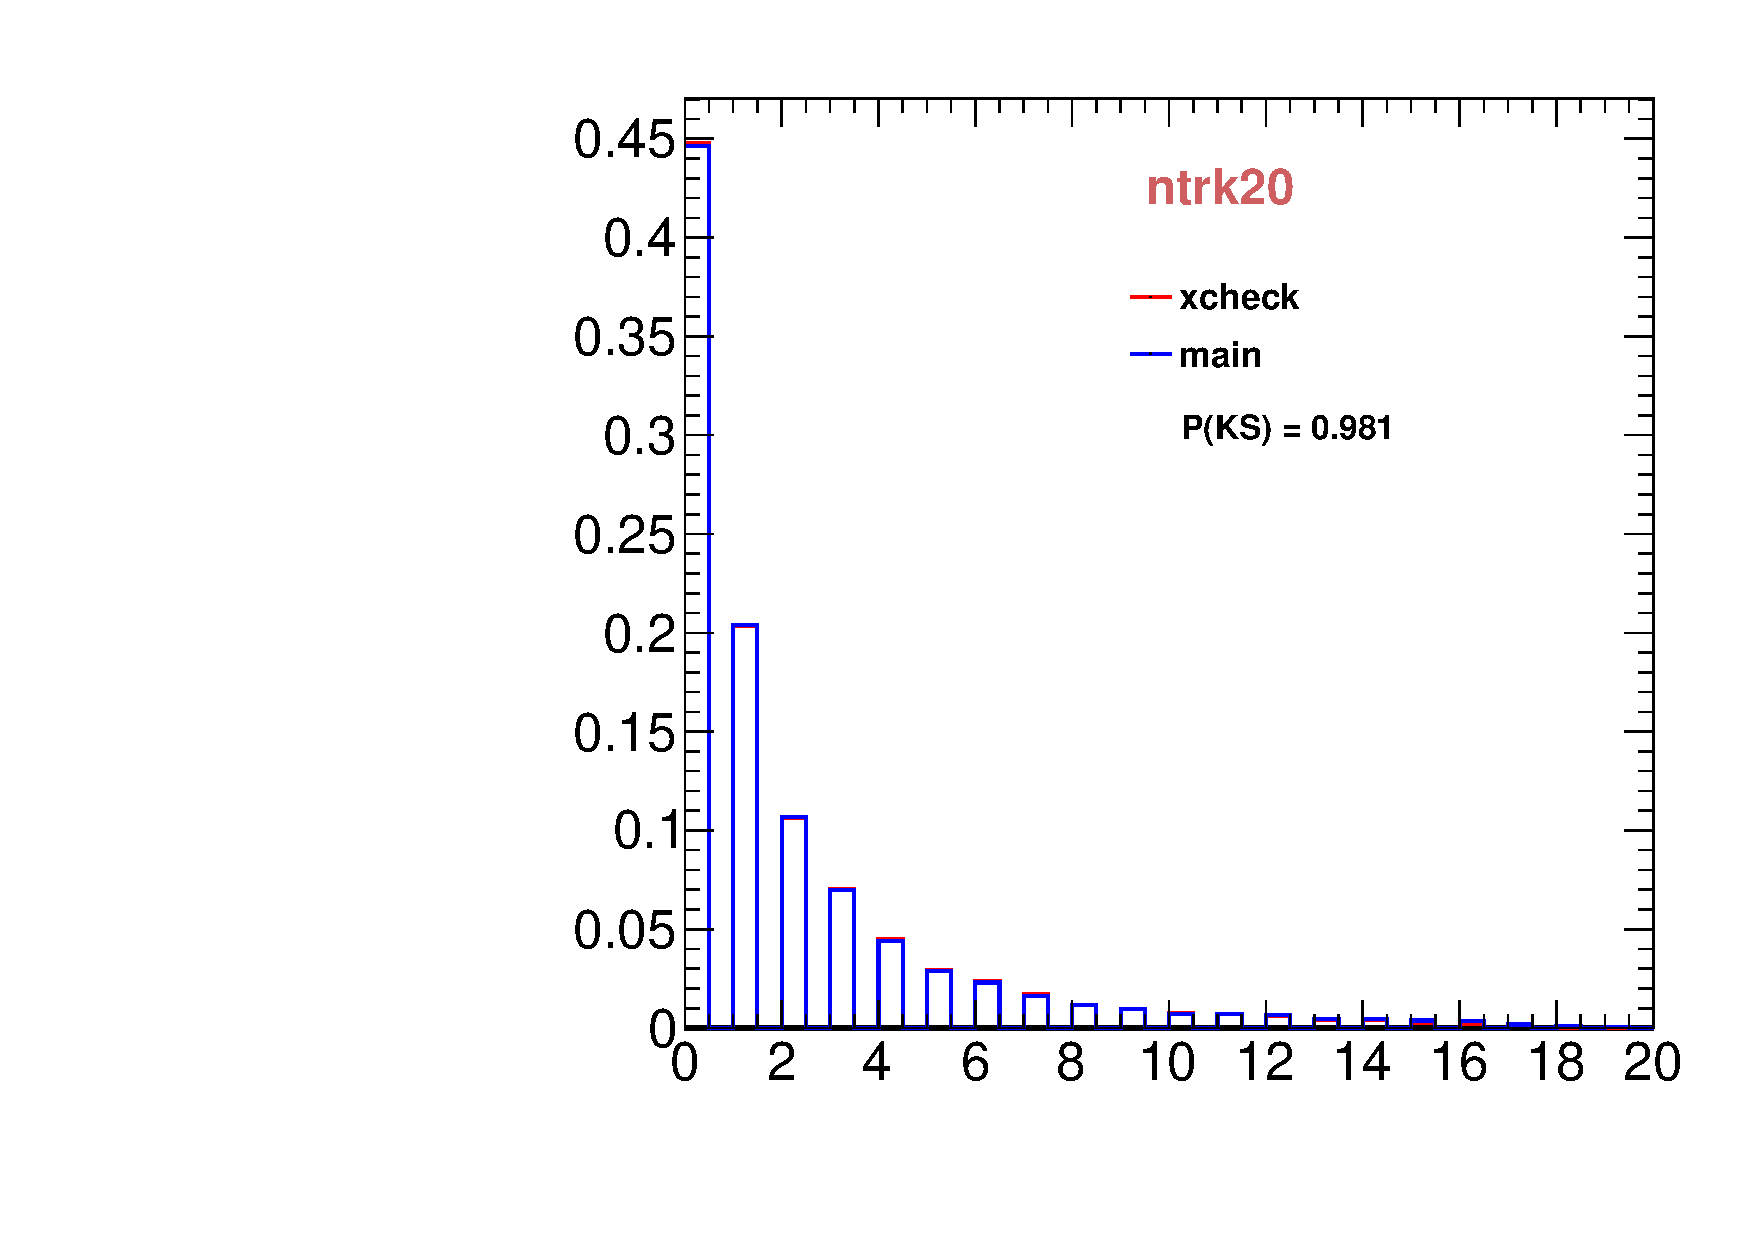
\includegraphics[width=0.3\textwidth]{Figures/VariablesComparison/MC_endcaps_figs/closetrk}
  %\label{fig:MC_endcaps_closetrk}
  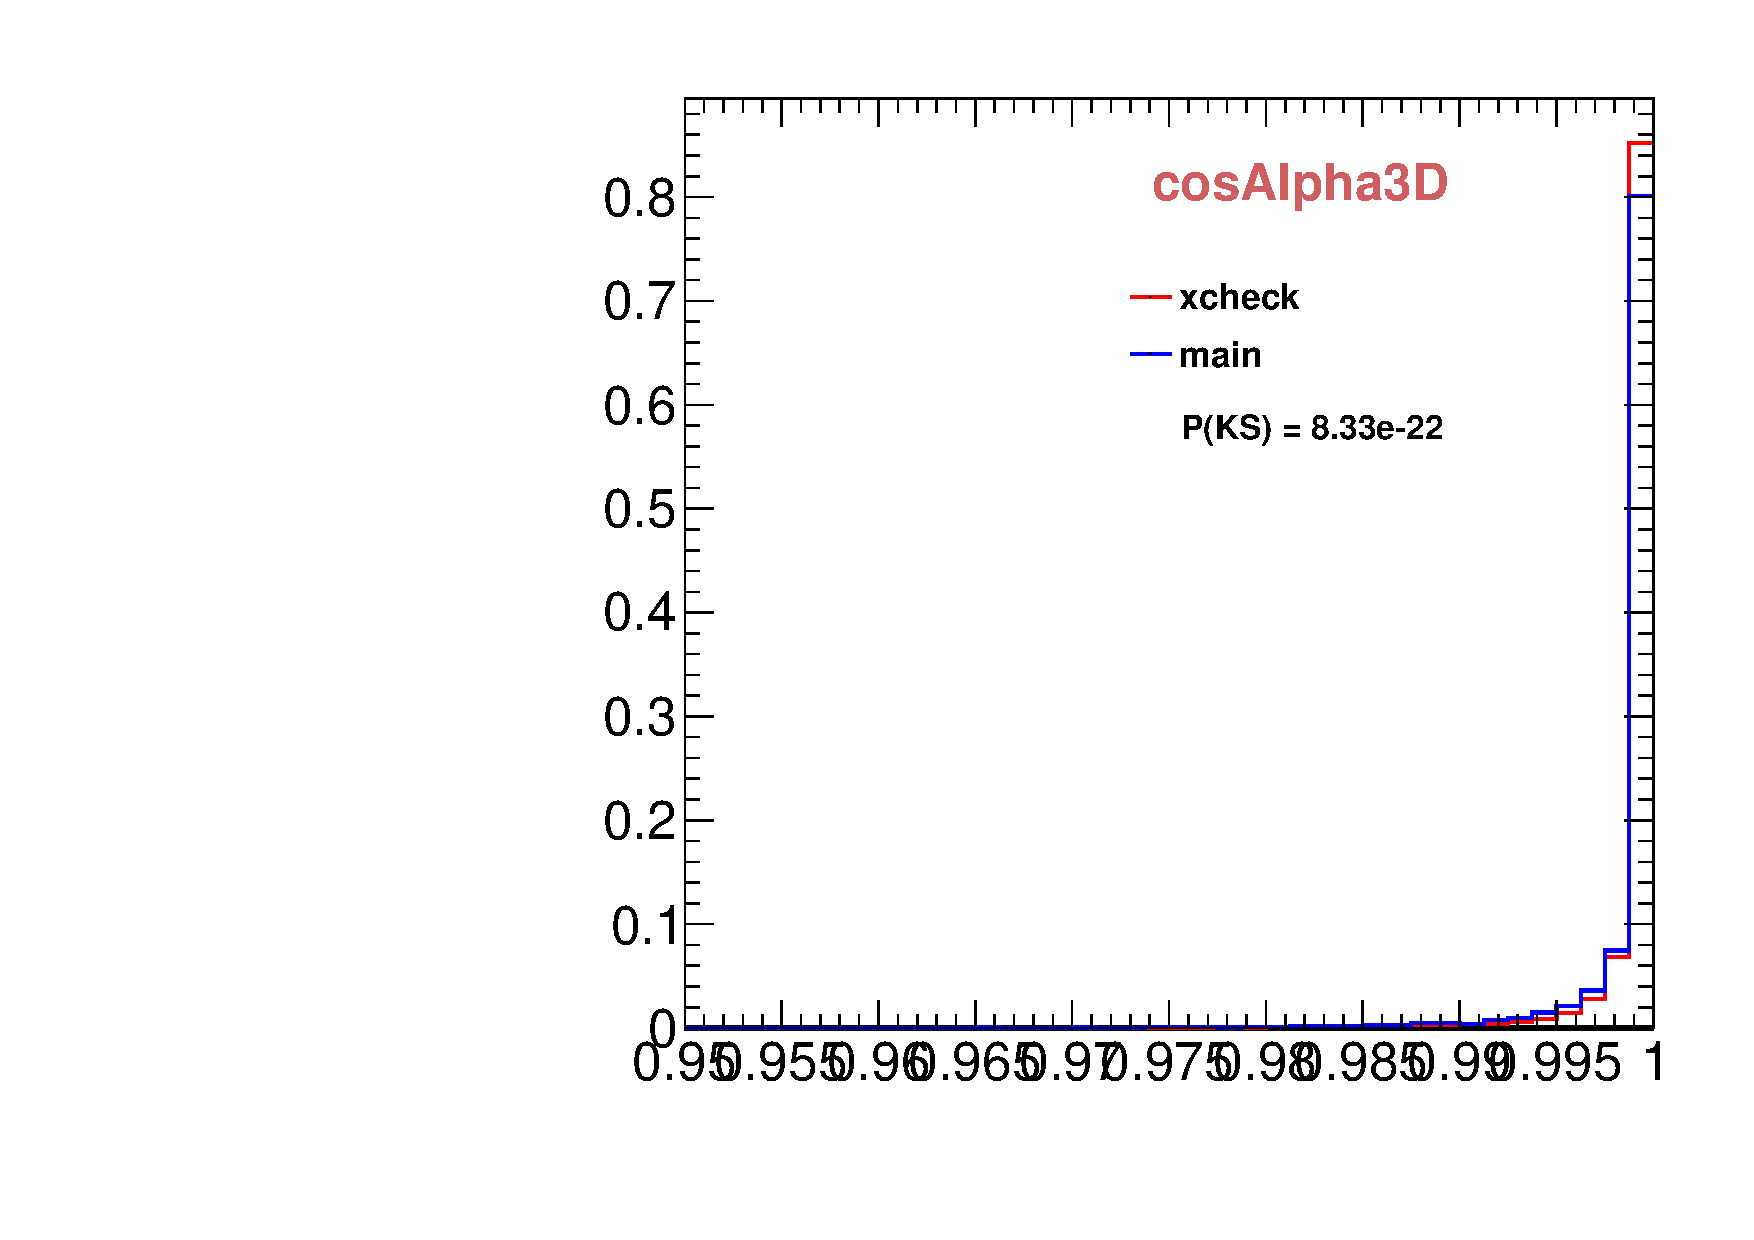
\includegraphics[width=0.3\textwidth]{Figures/VariablesComparison/MC_endcaps_figs/cosa}
  %\label{fig:MC_endcaps_cosa}
  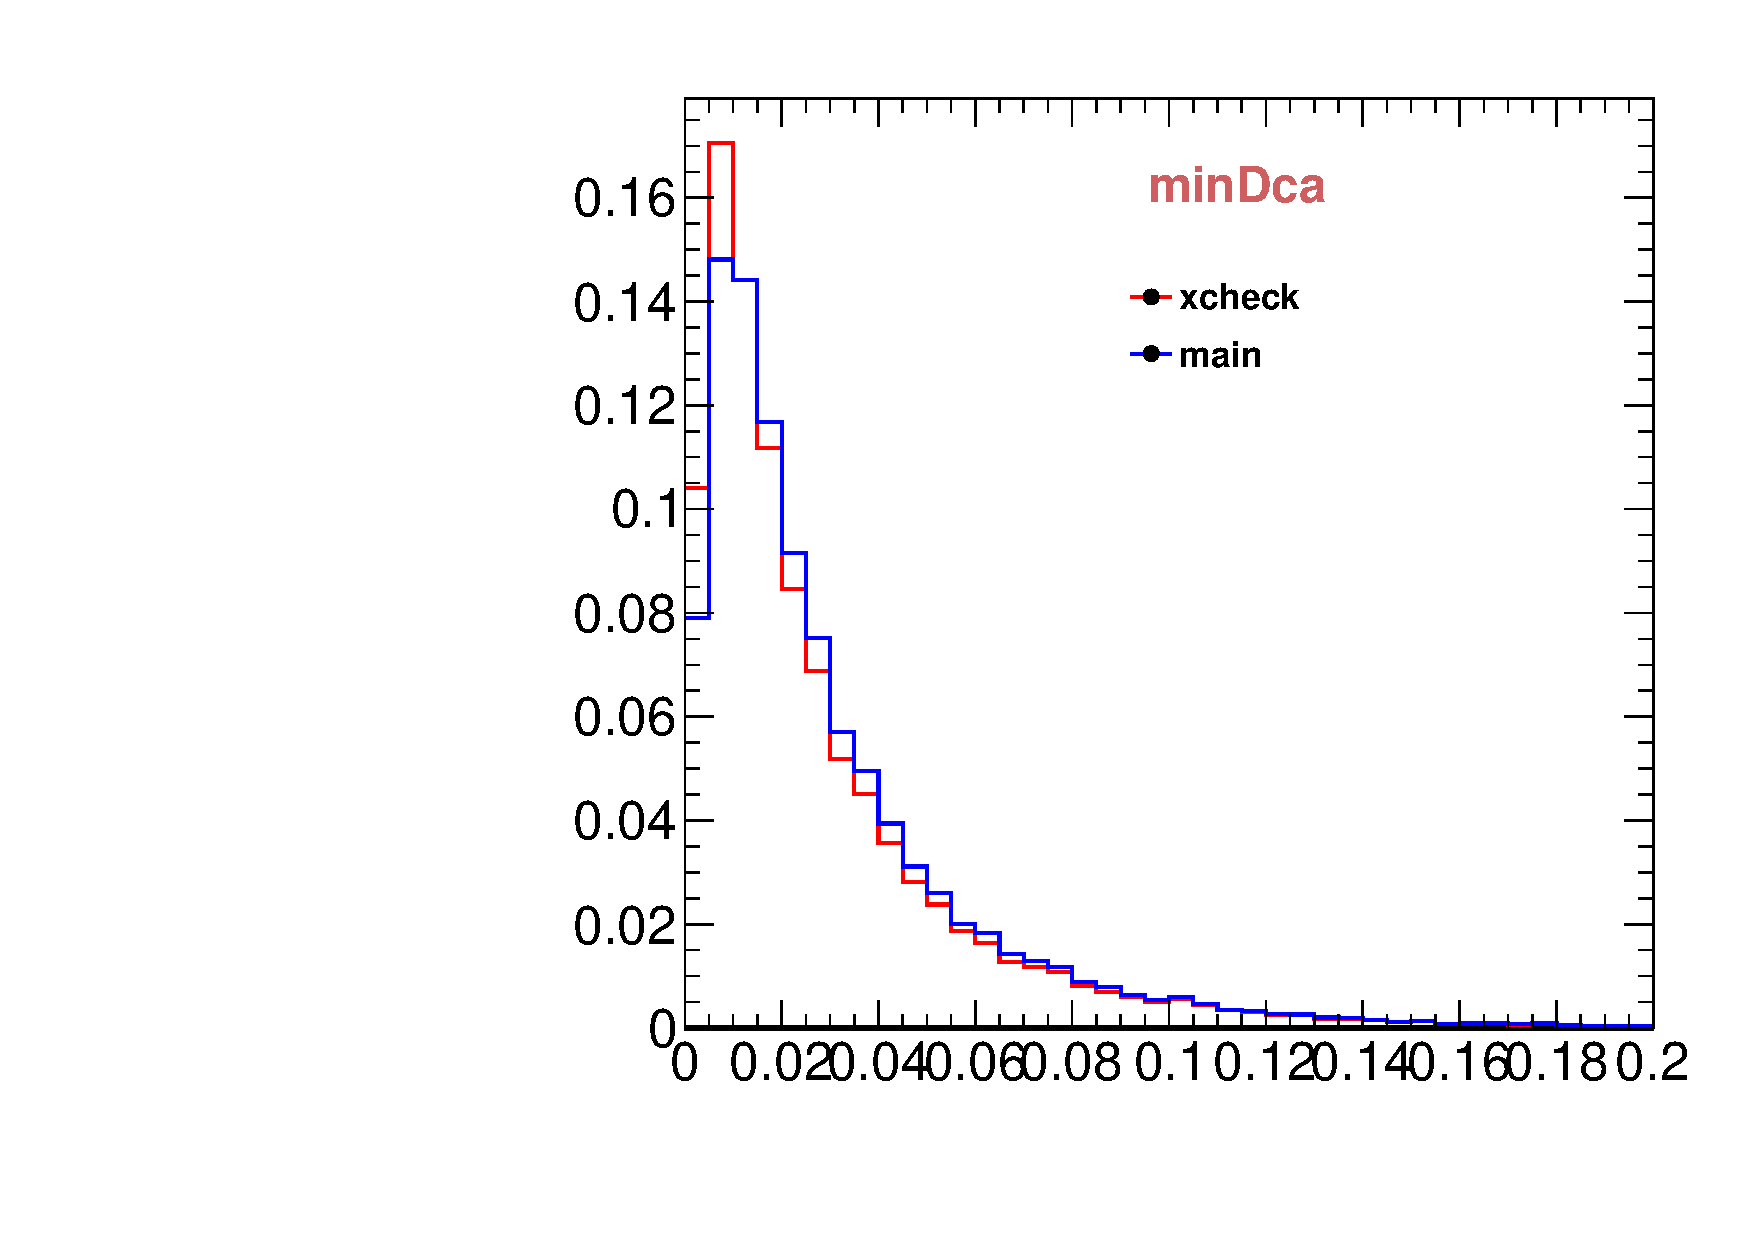
\includegraphics[width=0.3\textwidth]{Figures/VariablesComparison/MC_endcaps_figs/docatrk}
  %\label{fig:MC_endcaps_docatrk}
  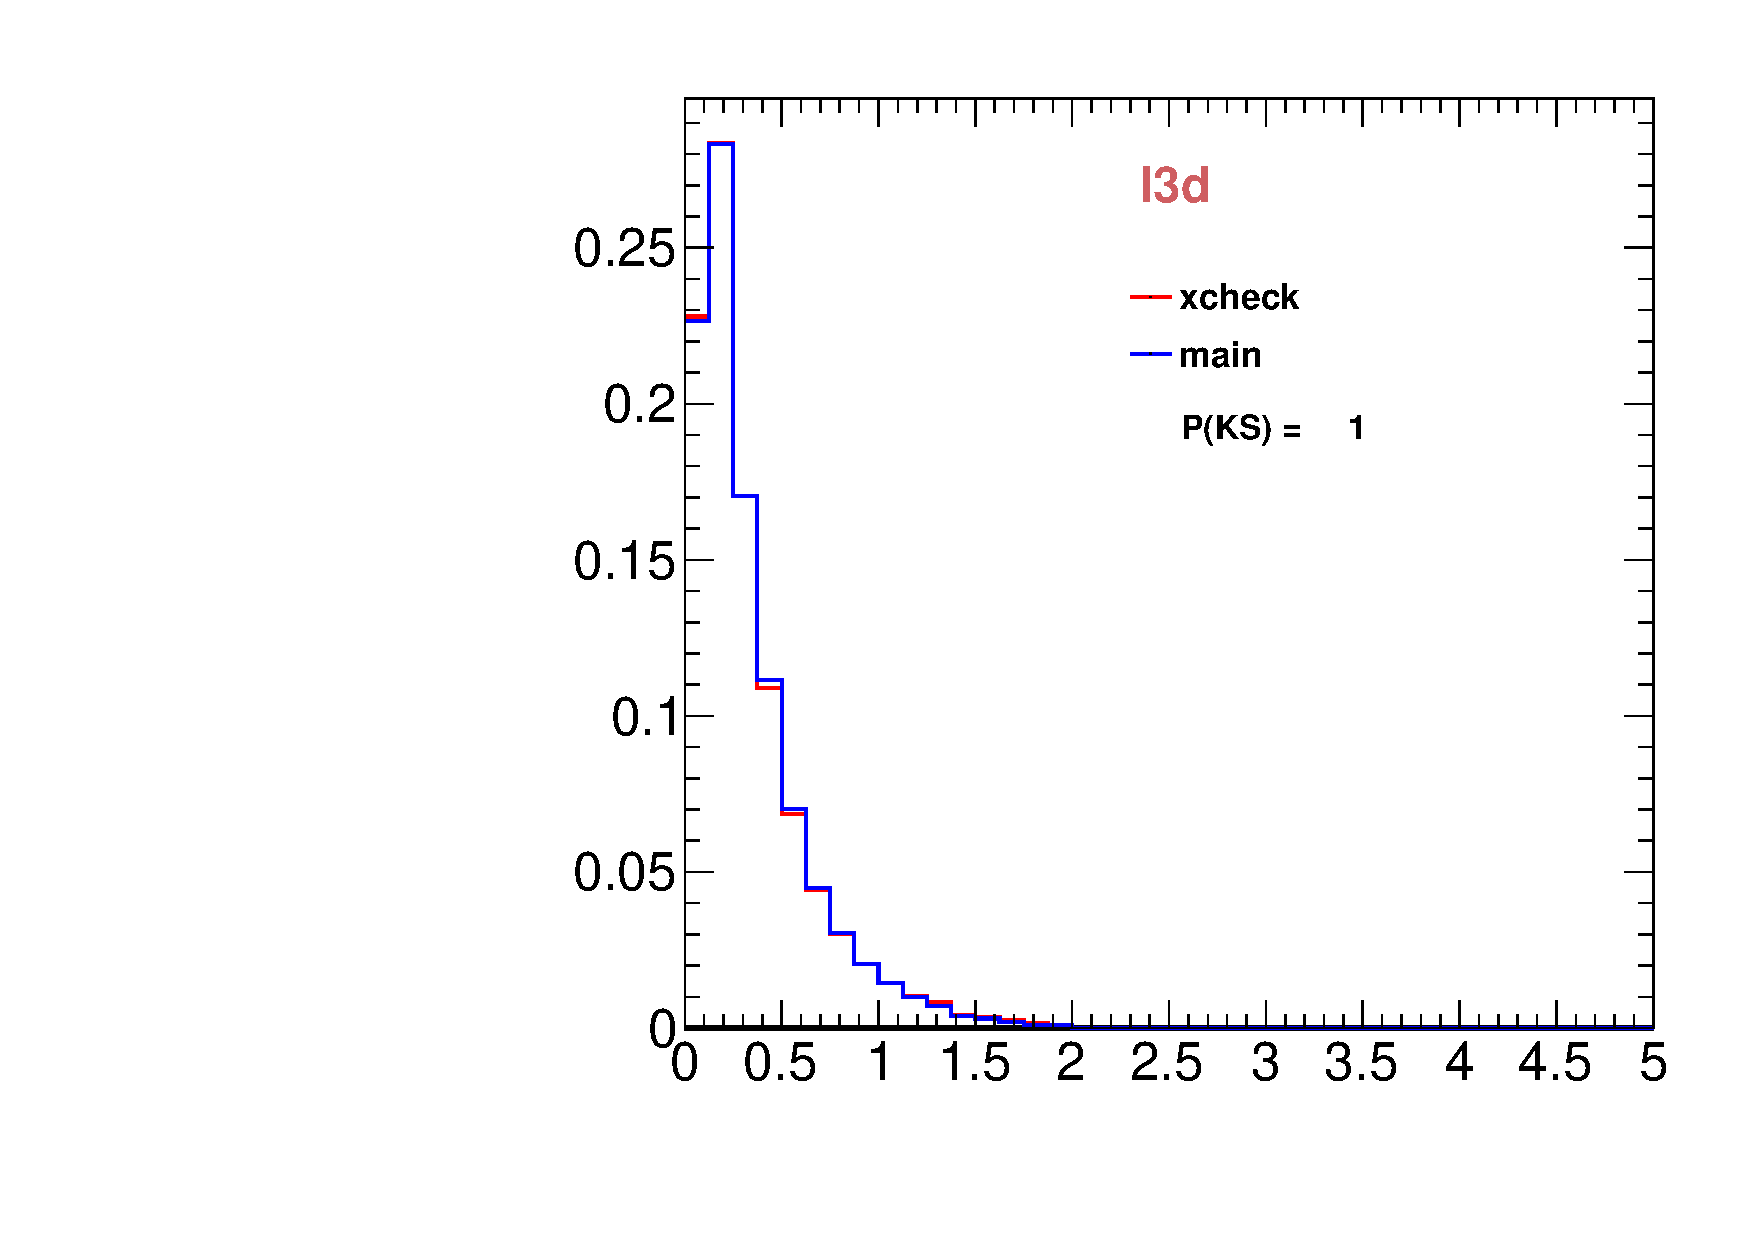
\includegraphics[width=0.3\textwidth]{Figures/VariablesComparison/MC_endcaps_figs/fl3d}
  %\label{fig:MC_endcaps_fl3d}
  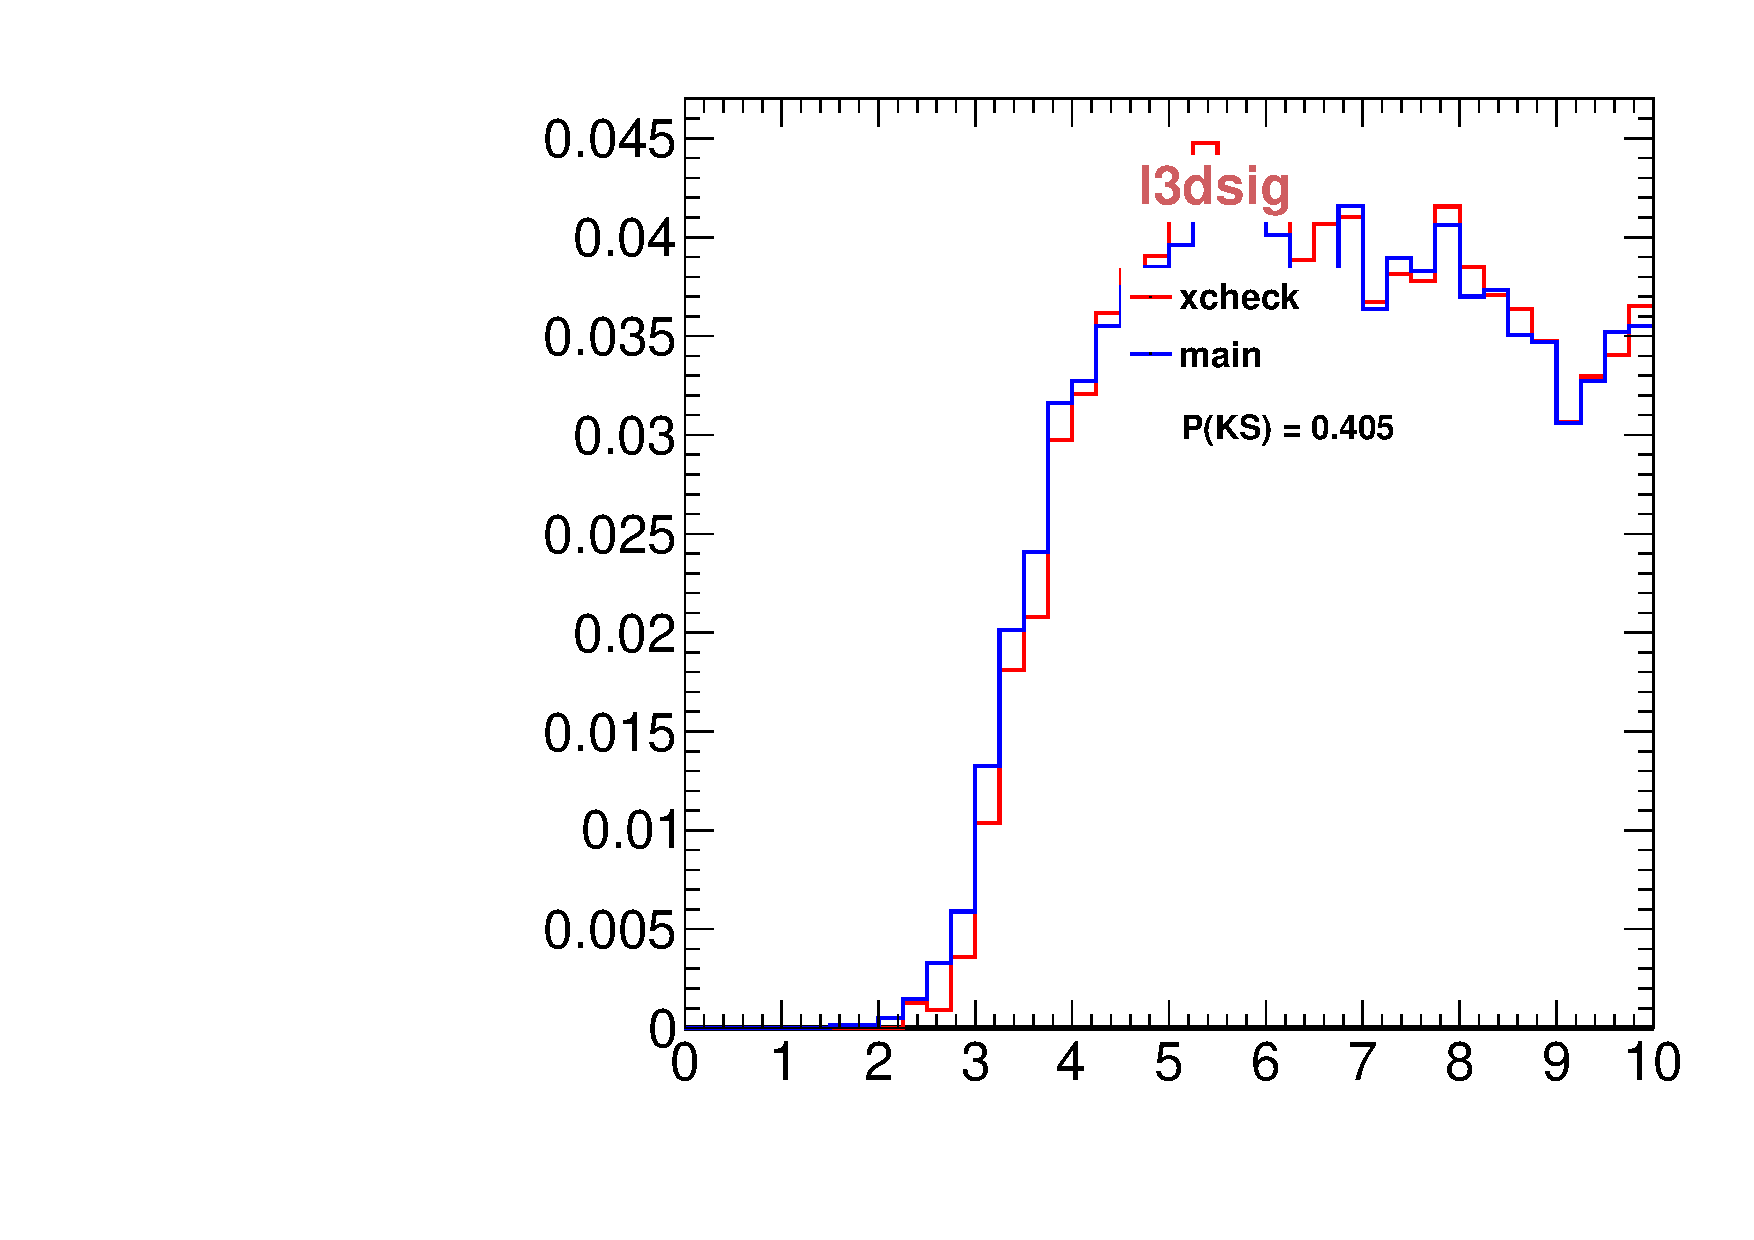
\includegraphics[width=0.3\textwidth]{Figures/VariablesComparison/MC_endcaps_figs/fls3d}
  %\label{fig:MC_endcaps_fls3d}
  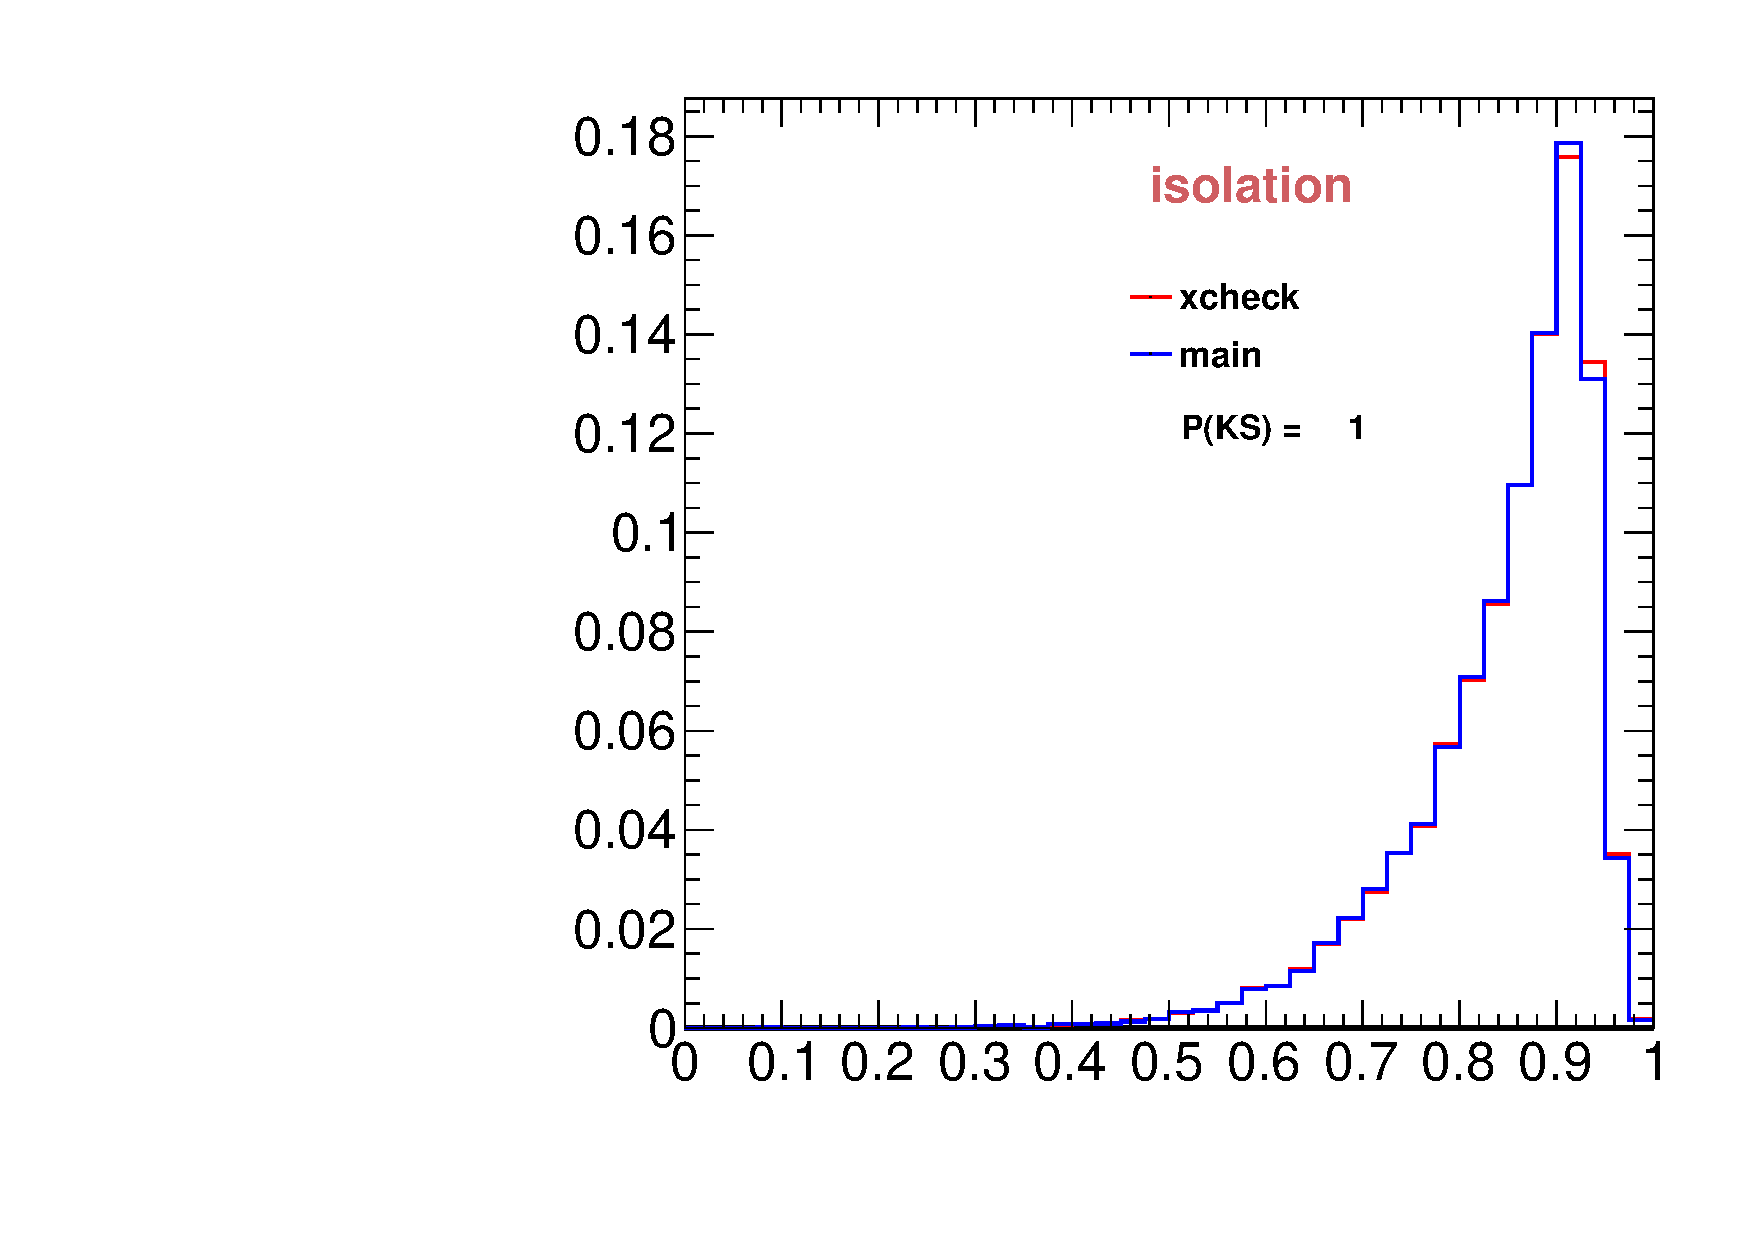
\includegraphics[width=0.3\textwidth]{Figures/VariablesComparison/MC_endcaps_figs/iso}
  %\label{fig:MC_endcaps_iso}
  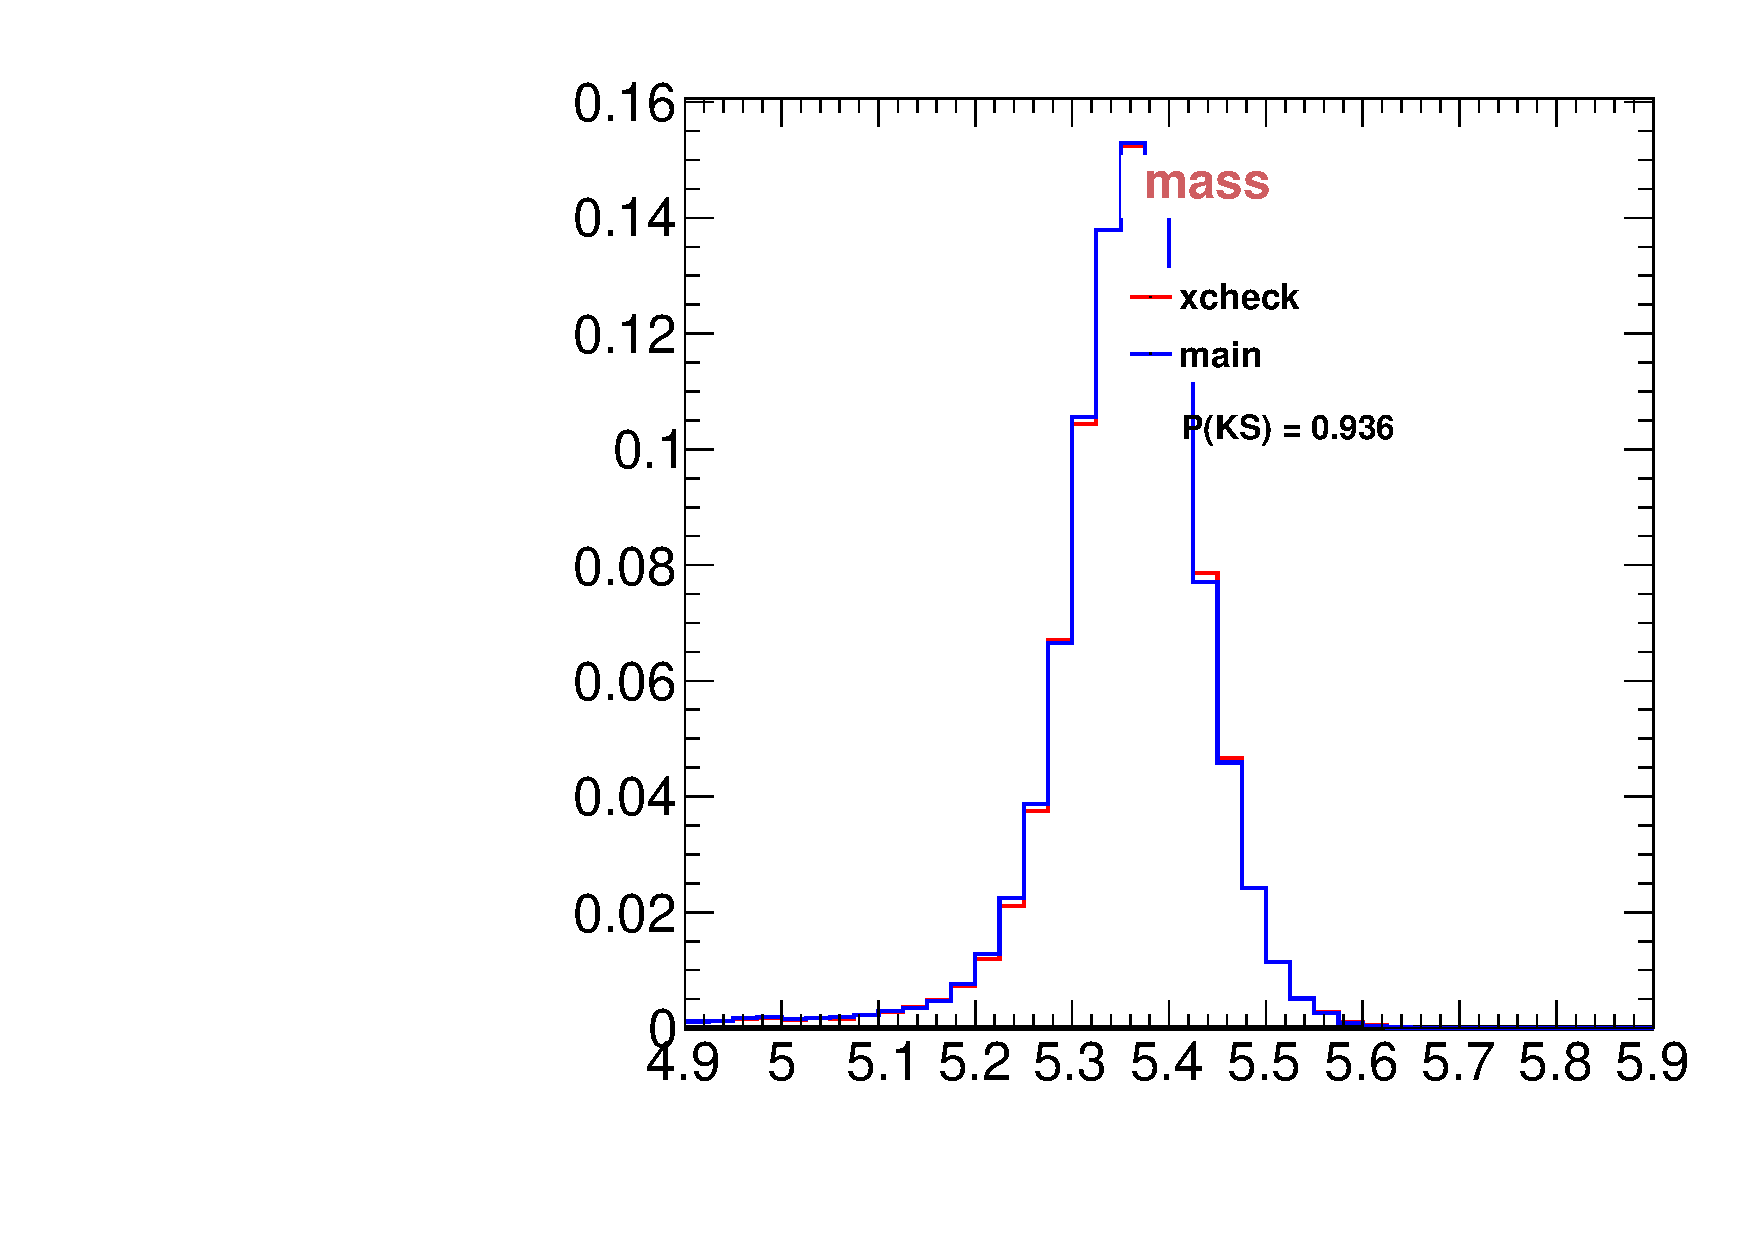
\includegraphics[width=0.3\textwidth]{Figures/VariablesComparison/MC_endcaps_figs/m}
  %\label{fig:MC_endcaps_m}
  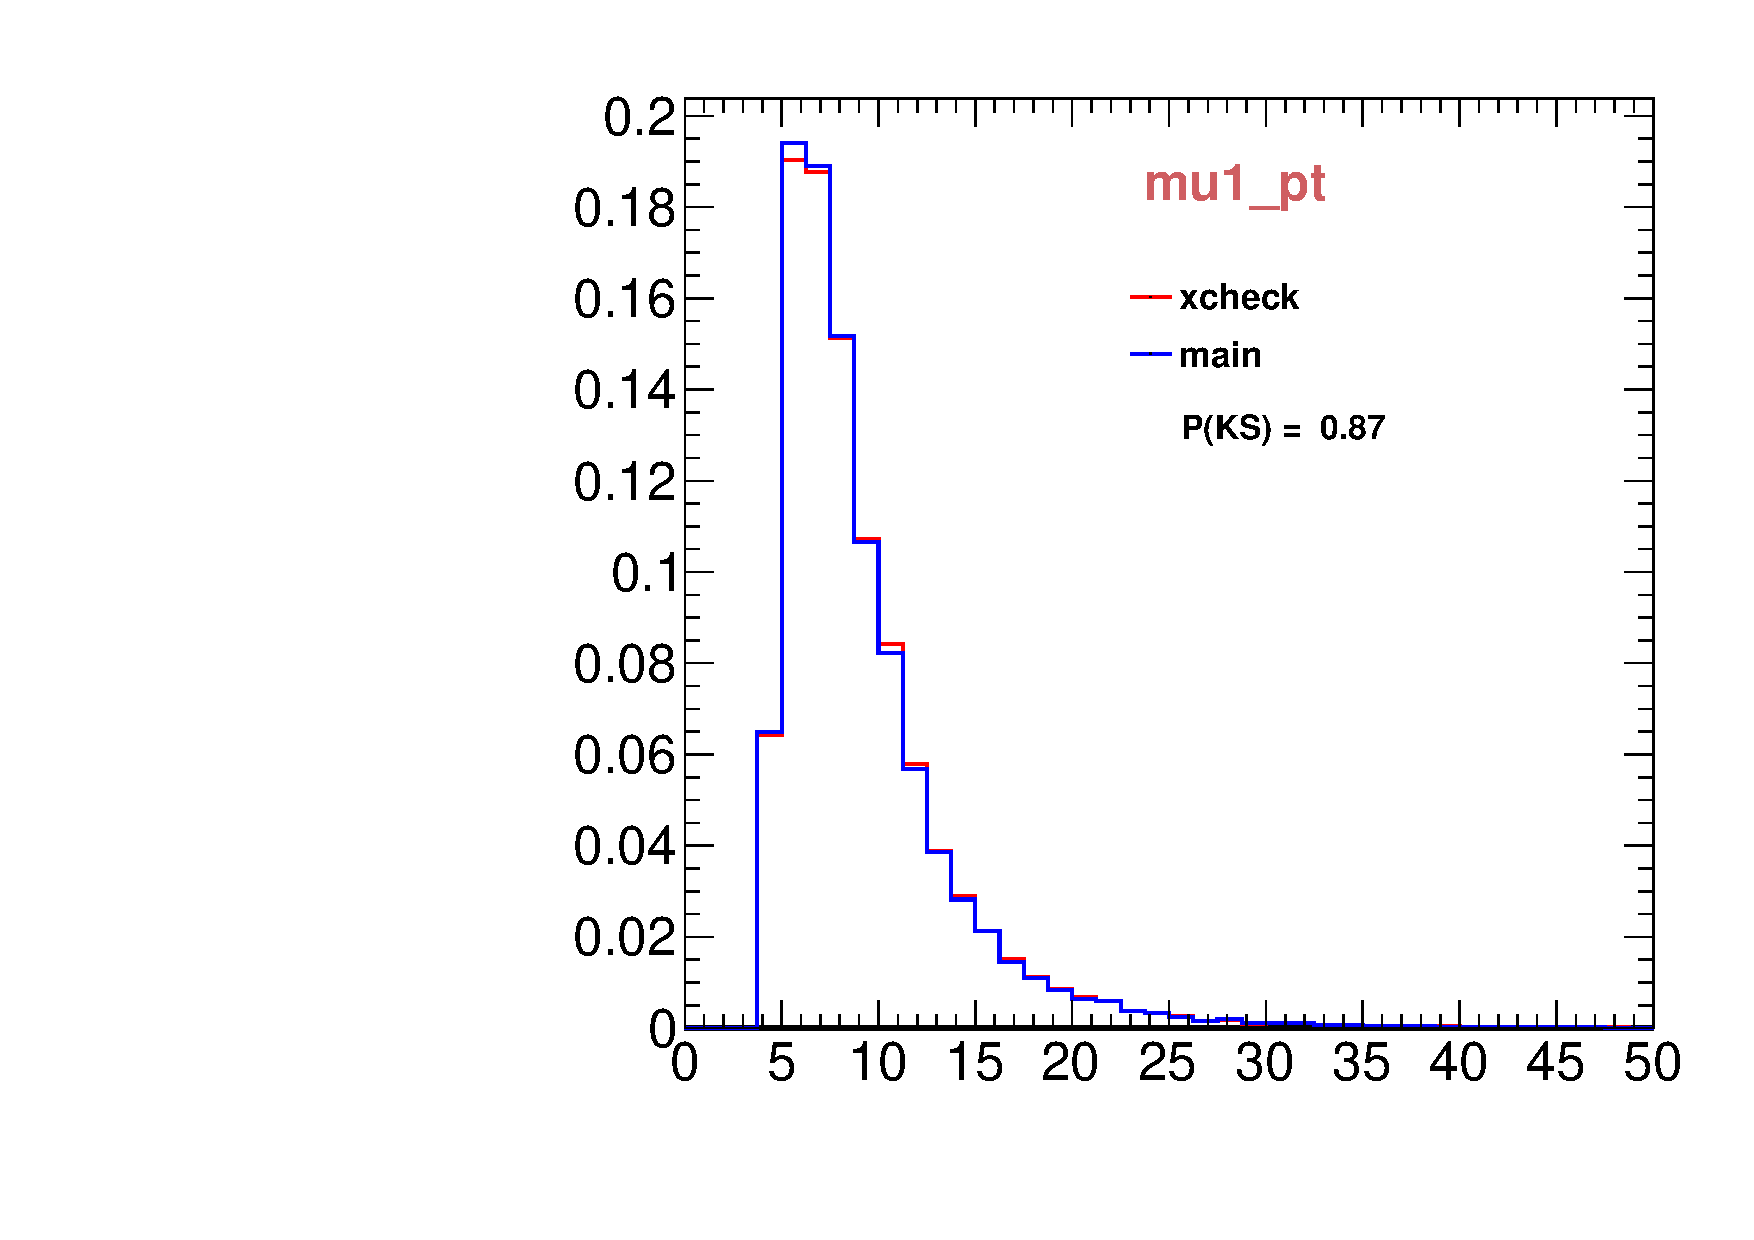
\includegraphics[width=0.3\textwidth]{Figures/VariablesComparison/MC_endcaps_figs/m1pt}
  %\label{fig:MC_endcaps_m1pt}
  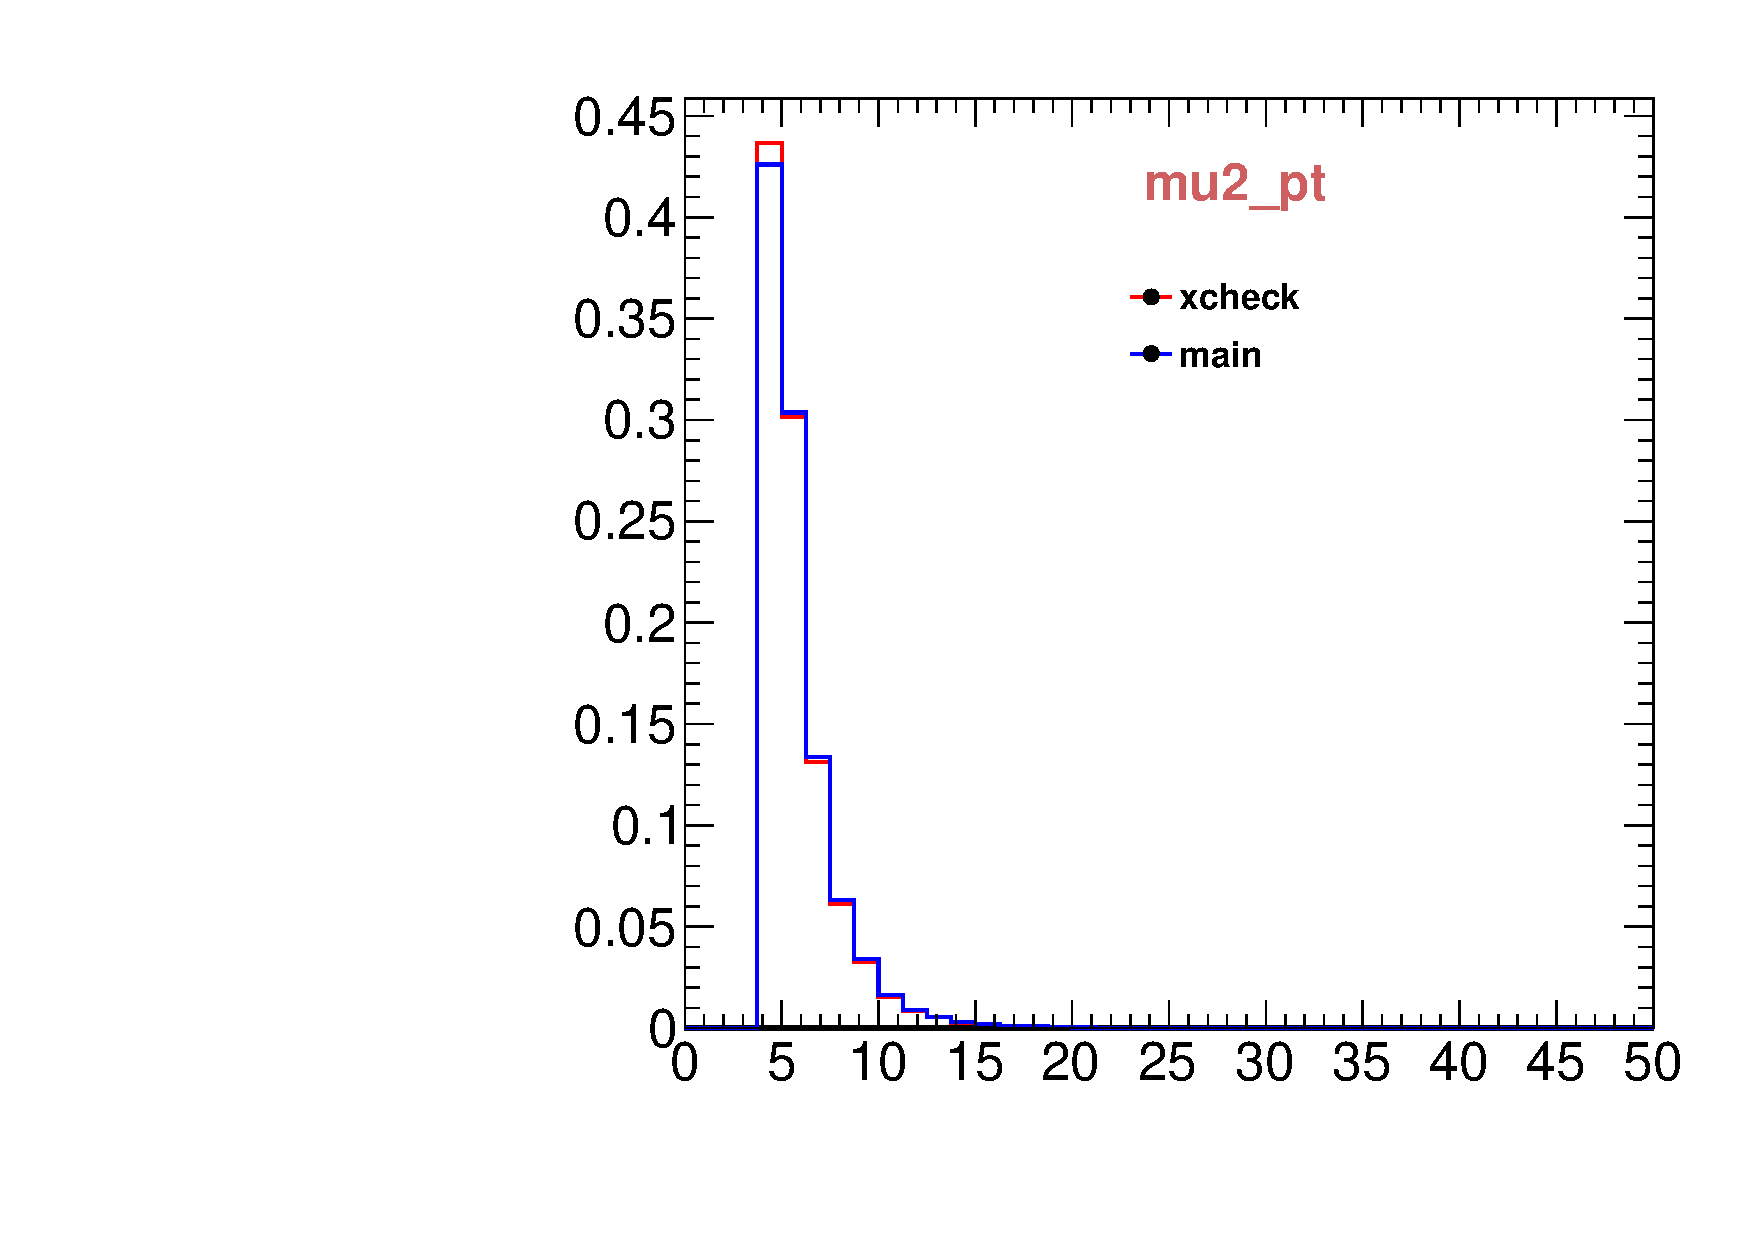
\includegraphics[width=0.3\textwidth]{Figures/VariablesComparison/MC_endcaps_figs/m2pt}
  %\label{fig:MC_endcaps_m2pt}
  \includegraphics[width=0.3\textwidth]{Figures/VariablesComparison/MC_endcaps_figs/maxdoca}
  %\label{fig:MC_endcaps_maxdoca}
  \includegraphics[width=0.3\textwidth]{Figures/VariablesComparison/MC_endcaps_figs/pt}
  %\label{fig:MC_endcaps_pt}
  \includegraphics[width=0.3\textwidth]{Figures/VariablesComparison/MC_endcaps_figs/pvip}
  %\label{fig:MC_endcaps_pvip}
  \includegraphics[width=0.3\textwidth]{Figures/VariablesComparison/MC_endcaps_figs/pvips}
  %\label{fig:MC_endcaps_pvips}
  \includegraphics[width=0.3\textwidth]{Figures/VariablesComparison/MC_endcaps_figs/pvw8}
  %\label{fig:MC_endcaps_pvw8}
  \includegraphics[width=0.3\textwidth]{Figures/VariablesComparison/MC_endcaps_figs/KS}
  %\label{fig:MC_endcaps_KS}
  \caption{Variable comparisons between the main analysis and the cross-check analysis. Part II: MC endcaps.}
  \label{fig:MC_endcaps_figs}
\end{figure}


\begin{figure}
  \centering
  \includegraphics[width=0.3\textwidth]{Figures/VariablesComparison/Data_barrel_figs/closetrk}
  %\label{fig:Data_barrel_closetrk}
  \includegraphics[width=0.3\textwidth]{Figures/VariablesComparison/Data_barrel_figs/cosa}
  %\label{fig:Data_barrel_cosa}
  \includegraphics[width=0.3\textwidth]{Figures/VariablesComparison/Data_barrel_figs/docatrk}
  %\label{fig:Data_barrel_docatrk}
  \includegraphics[width=0.3\textwidth]{Figures/VariablesComparison/Data_barrel_figs/fl3d}
  %\label{fig:Data_barrel_fl3d}
  \includegraphics[width=0.3\textwidth]{Figures/VariablesComparison/Data_barrel_figs/fls3d}
  %\label{fig:Data_barrel_fls3d}
  \includegraphics[width=0.3\textwidth]{Figures/VariablesComparison/Data_barrel_figs/iso}
  %\label{fig:Data_barrel_iso}
  \includegraphics[width=0.3\textwidth]{Figures/VariablesComparison/Data_barrel_figs/m}
  %\label{fig:Data_barrel_m}
  \includegraphics[width=0.3\textwidth]{Figures/VariablesComparison/Data_barrel_figs/m1pt}
  %\label{fig:Data_barrel_m1pt}
  \includegraphics[width=0.3\textwidth]{Figures/VariablesComparison/Data_barrel_figs/m2pt}
  %\label{fig:Data_barrel_m2pt}
  \includegraphics[width=0.3\textwidth]{Figures/VariablesComparison/Data_barrel_figs/maxdoca}
  %\label{fig:Data_barrel_maxdoca}
  \includegraphics[width=0.3\textwidth]{Figures/VariablesComparison/Data_barrel_figs/pt}
  %\label{fig:Data_barrel_pt}
  \includegraphics[width=0.3\textwidth]{Figures/VariablesComparison/Data_barrel_figs/pvip}
  %\label{fig:Data_barrel_pvip}
  \includegraphics[width=0.3\textwidth]{Figures/VariablesComparison/Data_barrel_figs/pvips}
  %\label{fig:Data_barrel_pvips}
  \includegraphics[width=0.3\textwidth]{Figures/VariablesComparison/Data_barrel_figs/pvw8}
  %\label{fig:Data_barrel_pvw8}
  \includegraphics[width=0.3\textwidth]{Figures/VariablesComparison/Data_barrel_figs/KS}
  %\label{fig:Data_barrel_KS}
  \caption{Variable comparisons between the main analysis and the cross-check analysis. Part III: Data barrel.}
  \label{fig:Data_barrel_figs}
\end{figure}


\begin{figure}
  \centering
  \includegraphics[width=0.3\textwidth]{Figures/VariablesComparison/Data_endcaps_figs/closetrk}
  %\label{fig:Data_endcaps_closetrk}
  \includegraphics[width=0.3\textwidth]{Figures/VariablesComparison/Data_endcaps_figs/cosa}
  %\label{fig:Data_endcaps_cosa}
  \includegraphics[width=0.3\textwidth]{Figures/VariablesComparison/Data_endcaps_figs/docatrk}
  %\label{fig:Data_endcaps_docatrk}
  \includegraphics[width=0.3\textwidth]{Figures/VariablesComparison/Data_endcaps_figs/fl3d}
  %\label{fig:Data_endcaps_fl3d}
  \includegraphics[width=0.3\textwidth]{Figures/VariablesComparison/Data_endcaps_figs/fls3d}
  %\label{fig:Data_endcaps_fls3d}
  \includegraphics[width=0.3\textwidth]{Figures/VariablesComparison/Data_endcaps_figs/iso}
  %\label{fig:Data_endcaps_iso}
  \includegraphics[width=0.3\textwidth]{Figures/VariablesComparison/Data_endcaps_figs/m}
  %\label{fig:Data_endcaps_m}
  \includegraphics[width=0.3\textwidth]{Figures/VariablesComparison/Data_endcaps_figs/m1pt}
  %\label{fig:Data_endcaps_m1pt}
  \includegraphics[width=0.3\textwidth]{Figures/VariablesComparison/Data_endcaps_figs/m2pt}
  %\label{fig:Data_endcaps_m2pt}
  \includegraphics[width=0.3\textwidth]{Figures/VariablesComparison/Data_endcaps_figs/maxdoca}
  %\label{fig:Data_endcaps_maxdoca}
  \includegraphics[width=0.3\textwidth]{Figures/VariablesComparison/Data_endcaps_figs/pt}
  %\label{fig:Data_endcaps_pt}
  \includegraphics[width=0.3\textwidth]{Figures/VariablesComparison/Data_endcaps_figs/pvip}
  %\label{fig:Data_endcaps_pvip}
  \includegraphics[width=0.3\textwidth]{Figures/VariablesComparison/Data_endcaps_figs/pvips}
  %\label{fig:Data_endcaps_pvips}
  \includegraphics[width=0.3\textwidth]{Figures/VariablesComparison/Data_endcaps_figs/pvw8}
  %\label{fig:Data_endcaps_pvw8}
  \includegraphics[width=0.3\textwidth]{Figures/VariablesComparison/Data_endcaps_figs/KS}
  %\label{fig:Data_endcaps_KS}
  \caption{Variable comparisons between the main analysis and the cross-check analysis. Part IV: Data endcaps.}
  \label{fig:Data_endcaps_figs}
\end{figure}



%\begin{sidewaysfigure}
        \centering
        \begin{subfigure}[b]{0.2\textwidth}
                \centering
                \includegraphics[width=\textwidth]{Figures/VariablesComparison/MC_barrel_figs_3h/ntrk}
                \label{fig:MC_barrel_ntrk_3h}
        \end{subfigure}
        \begin{subfigure}[b]{0.2\textwidth}
                \centering
                \includegraphics[width=\textwidth]{Figures/VariablesComparison/MC_barrel_figs_3h/cosAlpha3D}
                \label{fig:MC_barrel_cosAlpha3D_3h}
        \end{subfigure}
        \begin{subfigure}[b]{0.2\textwidth}
                \centering
                \includegraphics[width=\textwidth]{Figures/VariablesComparison/MC_barrel_figs_3h/minDca}
                \label{fig:MC_barrel_minDca_3h}
        \end{subfigure}
        \begin{subfigure}[b]{0.2\textwidth}
                \centering
                \includegraphics[width=\textwidth]{Figures/VariablesComparison/MC_barrel_figs_3h/l3d}
                \label{fig:MC_barrel_l3d_3h}
        \end{subfigure}
        \begin{subfigure}[b]{0.2\textwidth}
                \centering
                \includegraphics[width=\textwidth]{Figures/VariablesComparison/MC_barrel_figs_3h/l3dsig}
                \label{fig:MC_barrel_l3dsig_3h}
        \end{subfigure}
        \begin{subfigure}[b]{0.2\textwidth}
                \centering
                \includegraphics[width=\textwidth]{Figures/VariablesComparison/MC_barrel_figs_3h/isolation}
                \label{fig:MC_barrel_isolation_3h}
        \end{subfigure}
        \begin{subfigure}[b]{0.2\textwidth}
                \centering
                \includegraphics[width=\textwidth]{Figures/VariablesComparison/MC_barrel_figs_3h/mass}
                \label{fig:MC_barrel_mass_3h}
        \end{subfigure}
        \begin{subfigure}[b]{0.2\textwidth}
                \centering
                \includegraphics[width=\textwidth]{Figures/VariablesComparison/MC_barrel_figs_3h/mu1_pt}
                \label{fig:MC_barrel_mu1_pt_3h}
        \end{subfigure}
        \begin{subfigure}[b]{0.2\textwidth}
                \centering
                \includegraphics[width=\textwidth]{Figures/VariablesComparison/MC_barrel_figs_3h/mu2_pt}
                \label{fig:MC_barrel_mu2_pt_3h}
        \end{subfigure}
        \begin{subfigure}[b]{0.2\textwidth}
                \centering
                \includegraphics[width=\textwidth]{Figures/VariablesComparison/MC_barrel_figs_3h/dca}
                \label{fig:MC_barrel_dca_3h}
        \end{subfigure}
        \begin{subfigure}[b]{0.2\textwidth}
                \centering
                \includegraphics[width=\textwidth]{Figures/VariablesComparison/MC_barrel_figs_3h/pt}
                \label{fig:MC_barrel_pt_3h}
        \end{subfigure}
        \begin{subfigure}[b]{0.2\textwidth}
                \centering
                \includegraphics[width=\textwidth]{Figures/VariablesComparison/MC_barrel_figs_3h/delta3d}
                \label{fig:MC_barrel_delta3d_3h}
        \end{subfigure}
        \begin{subfigure}[b]{0.2\textwidth}
                \centering
                \includegraphics[width=\textwidth]{Figures/VariablesComparison/MC_barrel_figs_3h/delta3dErr}
                \label{fig:MC_barrel_delta3d/delta3dErr_3h}
        \end{subfigure}
        \begin{subfigure}[b]{0.2\textwidth}
                \centering
                \includegraphics[width=\textwidth]{Figures/VariablesComparison/MC_barrel_figs_3h/pvw8}
                \label{fig:MC_barrel_pvw8_3h}
        \end{subfigure}
        \begin{subfigure}[b]{0.2\textwidth}
                \centering
                \includegraphics[width=\textwidth]{Figures/VariablesComparison/MC_barrel_figs_3h/KS}
                \label{fig:MC_barrel_KS_3h}
        \end{subfigure}
        \caption{Overlay of BDT training variable distributions in Signal MC for events of the three subsets in the barrel. The plot on the bottom right summarizes all KS probablities.}
        \label{fig:MC_barrel_figs_3h}
\end{sidewaysfigure}


\begin{sidewaysfigure}
        \centering
        \begin{subfigure}[b]{0.2\textwidth}
                \centering
                \includegraphics[width=\textwidth]{Figures/VariablesComparison/MC_endcaps_figs_3h/ntrk}
                \label{fig:MC_endcaps_ntrk_3h}
        \end{subfigure}
        \begin{subfigure}[b]{0.2\textwidth}
                \centering
                \includegraphics[width=\textwidth]{Figures/VariablesComparison/MC_endcaps_figs_3h/cosAlpha3D}
                \label{fig:MC_endcaps_cosAlpha3D_3h}
        \end{subfigure}
        \begin{subfigure}[b]{0.2\textwidth}
                \centering
                \includegraphics[width=\textwidth]{Figures/VariablesComparison/MC_endcaps_figs_3h/minDca}
                \label{fig:MC_endcaps_minDca_3h}
        \end{subfigure}
        \begin{subfigure}[b]{0.2\textwidth}
                \centering
                \includegraphics[width=\textwidth]{Figures/VariablesComparison/MC_endcaps_figs_3h/l3d}
                \label{fig:MC_endcaps_l3d_3h}
        \end{subfigure}
        \begin{subfigure}[b]{0.2\textwidth}
                \centering
                \includegraphics[width=\textwidth]{Figures/VariablesComparison/MC_endcaps_figs_3h/l3dsig}
                \label{fig:MC_endcaps_l3dsig_3h}
        \end{subfigure}
        \begin{subfigure}[b]{0.2\textwidth}
                \centering
                \includegraphics[width=\textwidth]{Figures/VariablesComparison/MC_endcaps_figs_3h/isolation}
                \label{fig:MC_endcaps_isolation_3h}
        \end{subfigure}
        \begin{subfigure}[b]{0.2\textwidth}
                \centering
                \includegraphics[width=\textwidth]{Figures/VariablesComparison/MC_endcaps_figs_3h/mass}
                \label{fig:MC_endcaps_mass_3h}
        \end{subfigure}
        \begin{subfigure}[b]{0.2\textwidth}
                \centering
                \includegraphics[width=\textwidth]{Figures/VariablesComparison/MC_endcaps_figs_3h/mu1_pt}
                \label{fig:MC_endcaps_mu1_pt_3h}
        \end{subfigure}
        \begin{subfigure}[b]{0.2\textwidth}
                \centering
                \includegraphics[width=\textwidth]{Figures/VariablesComparison/MC_endcaps_figs_3h/mu2_pt}
                \label{fig:MC_endcaps_mu2_pt_3h}
        \end{subfigure}
        \begin{subfigure}[b]{0.2\textwidth}
                \centering
                \includegraphics[width=\textwidth]{Figures/VariablesComparison/MC_endcaps_figs_3h/dca}
                \label{fig:MC_endcaps_dca_3h}
        \end{subfigure}
        \begin{subfigure}[b]{0.2\textwidth}
                \centering
                \includegraphics[width=\textwidth]{Figures/VariablesComparison/MC_endcaps_figs_3h/pt}
                \label{fig:MC_endcaps_pt_3h}
        \end{subfigure}
        \begin{subfigure}[b]{0.2\textwidth}
                \centering
                \includegraphics[width=\textwidth]{Figures/VariablesComparison/MC_endcaps_figs_3h/delta3d}
                \label{fig:MC_endcaps_delta3d_3h}
        \end{subfigure}
        \begin{subfigure}[b]{0.2\textwidth}
                \centering
                \includegraphics[width=\textwidth]{Figures/VariablesComparison/MC_endcaps_figs_3h/delta3dErr}
                \label{fig:MC_endcaps_delta3d/delta3dErr_3h}
        \end{subfigure}
        \begin{subfigure}[b]{0.2\textwidth}
                \centering
                \includegraphics[width=\textwidth]{Figures/VariablesComparison/MC_endcaps_figs_3h/pvw8}
                \label{fig:MC_endcaps_pvw8_3h}
        \end{subfigure}
        \begin{subfigure}[b]{0.2\textwidth}
                \centering
                \includegraphics[width=\textwidth]{Figures/VariablesComparison/MC_endcaps_figs_3h/KS}
                \label{fig:MC_endcaps_KS_3h}
        \end{subfigure}
        \caption{Overlay of BDT training variable distributions in Signal MC for events of the three subsets in the endcap. The plot on the bottom right summarizes all KS probablities.}
        \label{fig:MC_endcaps_figs_3h}
\end{sidewaysfigure}


\begin{sidewaysfigure}
        \centering
        \begin{subfigure}[b]{0.2\textwidth}
                \centering
                \includegraphics[width=\textwidth]{Figures/VariablesComparison/Data_barrel_figs_3h/ntrk}
                \label{fig:Data_barrel_ntrk_3h}
        \end{subfigure}
        \begin{subfigure}[b]{0.2\textwidth}
                \centering
                \includegraphics[width=\textwidth]{Figures/VariablesComparison/Data_barrel_figs_3h/cosAlpha3D}
                \label{fig:Data_barrel_cosAlpha3D_3h}
        \end{subfigure}
        \begin{subfigure}[b]{0.2\textwidth}
                \centering
                \includegraphics[width=\textwidth]{Figures/VariablesComparison/Data_barrel_figs_3h/minDca}
                \label{fig:Data_barrel_minDca_3h}
        \end{subfigure}
        \begin{subfigure}[b]{0.2\textwidth}
                \centering
                \includegraphics[width=\textwidth]{Figures/VariablesComparison/Data_barrel_figs_3h/l3d}
                \label{fig:Data_barrel_l3d_3h}
        \end{subfigure}
        \begin{subfigure}[b]{0.2\textwidth}
                \centering
                \includegraphics[width=\textwidth]{Figures/VariablesComparison/Data_barrel_figs_3h/l3dsig}
                \label{fig:Data_barrel_l3dsig_3h}
        \end{subfigure}
        \begin{subfigure}[b]{0.2\textwidth}
                \centering
                \includegraphics[width=\textwidth]{Figures/VariablesComparison/Data_barrel_figs_3h/isolation}
                \label{fig:Data_barrel_isolation_3h}
        \end{subfigure}
        \begin{subfigure}[b]{0.2\textwidth}
                \centering
                \includegraphics[width=\textwidth]{Figures/VariablesComparison/Data_barrel_figs_3h/mass}
                \label{fig:Data_barrel_mass_3h}
        \end{subfigure}
        \begin{subfigure}[b]{0.2\textwidth}
                \centering
                \includegraphics[width=\textwidth]{Figures/VariablesComparison/Data_barrel_figs_3h/mu1_pt}
                \label{fig:Data_barrel_mu1_pt_3h}
        \end{subfigure}
        \begin{subfigure}[b]{0.2\textwidth}
                \centering
                \includegraphics[width=\textwidth]{Figures/VariablesComparison/Data_barrel_figs_3h/mu2_pt}
                \label{fig:Data_barrel_mu2_pt_3h}
        \end{subfigure}
        \begin{subfigure}[b]{0.2\textwidth}
                \centering
                \includegraphics[width=\textwidth]{Figures/VariablesComparison/Data_barrel_figs_3h/dca}
                \label{fig:Data_barrel_dca_3h}
        \end{subfigure}
        \begin{subfigure}[b]{0.2\textwidth}
                \centering
                \includegraphics[width=\textwidth]{Figures/VariablesComparison/Data_barrel_figs_3h/pt}
                \label{fig:Data_barrel_pt_3h}
        \end{subfigure}
        \begin{subfigure}[b]{0.2\textwidth}
                \centering
                \includegraphics[width=\textwidth]{Figures/VariablesComparison/Data_barrel_figs_3h/delta3d}
                \label{fig:Data_barrel_delta3d_3h}
        \end{subfigure}
        \begin{subfigure}[b]{0.2\textwidth}
                \centering
                \includegraphics[width=\textwidth]{Figures/VariablesComparison/Data_barrel_figs_3h/delta3dErr}
                \label{fig:Data_barrel_delta3d/delta3dErr_3h}
        \end{subfigure}
        \begin{subfigure}[b]{0.2\textwidth}
                \centering
                \includegraphics[width=\textwidth]{Figures/VariablesComparison/Data_barrel_figs_3h/pvw8}
                \label{fig:Data_barrel_pvw8_3h}
        \end{subfigure}
        \begin{subfigure}[b]{0.2\textwidth}
                \centering
                \includegraphics[width=\textwidth]{Figures/VariablesComparison/Data_barrel_figs_3h/KS}
                \label{fig:Data_barrel_KS_3h}
        \end{subfigure}
        \caption{Overlay of BDT training variable distributions in data sideband background for events of the three subsets in the barrel. The plot on the bottom right summarizes all KS probablities.}
        \label{fig:Data_barrel_figs_3h}
\end{sidewaysfigure}


\begin{sidewaysfigure}
        \centering
        \begin{subfigure}[b]{0.2\textwidth}
                \centering
                \includegraphics[width=\textwidth]{Figures/VariablesComparison/Data_endcaps_figs_3h/ntrk}
                \label{fig:Data_endcaps_ntrk_3h}
        \end{subfigure}
        \begin{subfigure}[b]{0.2\textwidth}
                \centering
                \includegraphics[width=\textwidth]{Figures/VariablesComparison/Data_endcaps_figs_3h/cosAlpha3D}
                \label{fig:Data_endcaps_cosAlpha3D_3h}
        \end{subfigure}
        \begin{subfigure}[b]{0.2\textwidth}
                \centering
                \includegraphics[width=\textwidth]{Figures/VariablesComparison/Data_endcaps_figs_3h/minDca}
                \label{fig:Data_endcaps_minDca_3h}
        \end{subfigure}
        \begin{subfigure}[b]{0.2\textwidth}
                \centering
                \includegraphics[width=\textwidth]{Figures/VariablesComparison/Data_endcaps_figs_3h/l3d}
                \label{fig:Data_endcaps_l3d_3h}
        \end{subfigure}
        \begin{subfigure}[b]{0.2\textwidth}
                \centering
                \includegraphics[width=\textwidth]{Figures/VariablesComparison/Data_endcaps_figs_3h/l3dsig}
                \label{fig:Data_endcaps_l3dsig_3h}
        \end{subfigure}
        \begin{subfigure}[b]{0.2\textwidth}
                \centering
                \includegraphics[width=\textwidth]{Figures/VariablesComparison/Data_endcaps_figs_3h/isolation}
                \label{fig:Data_endcaps_isolation_3h}
        \end{subfigure}
        \begin{subfigure}[b]{0.2\textwidth}
                \centering
                \includegraphics[width=\textwidth]{Figures/VariablesComparison/Data_endcaps_figs_3h/mass}
                \label{fig:Data_endcaps_mass_3h}
        \end{subfigure}
        \begin{subfigure}[b]{0.2\textwidth}
                \centering
                \includegraphics[width=\textwidth]{Figures/VariablesComparison/Data_endcaps_figs_3h/mu1_pt}
                \label{fig:Data_endcaps_mu1_pt_3h}
        \end{subfigure}
        \begin{subfigure}[b]{0.2\textwidth}
                \centering
                \includegraphics[width=\textwidth]{Figures/VariablesComparison/Data_endcaps_figs_3h/mu2_pt}
                \label{fig:Data_endcaps_mu2_pt_3h}
        \end{subfigure}
        \begin{subfigure}[b]{0.2\textwidth}
                \centering
                \includegraphics[width=\textwidth]{Figures/VariablesComparison/Data_endcaps_figs_3h/dca}
                \label{fig:Data_endcaps_dca_3h}
        \end{subfigure}
        \begin{subfigure}[b]{0.2\textwidth}
                \centering
                \includegraphics[width=\textwidth]{Figures/VariablesComparison/Data_endcaps_figs_3h/pt}
                \label{fig:Data_endcaps_pt_3h}
        \end{subfigure}
        \begin{subfigure}[b]{0.2\textwidth}
                \centering
                \includegraphics[width=\textwidth]{Figures/VariablesComparison/Data_endcaps_figs_3h/delta3d}
                \label{fig:Data_endcaps_delta3d_3h}
        \end{subfigure}
        \begin{subfigure}[b]{0.2\textwidth}
                \centering
                \includegraphics[width=\textwidth]{Figures/VariablesComparison/Data_endcaps_figs_3h/delta3dErr}
                \label{fig:Data_endcaps_delta3d/delta3dErr_3h}
        \end{subfigure}
        \begin{subfigure}[b]{0.2\textwidth}
                \centering
                \includegraphics[width=\textwidth]{Figures/VariablesComparison/Data_endcaps_figs_3h/pvw8}
                \label{fig:Data_endcaps_pvw8_3h}
        \end{subfigure}
        \begin{subfigure}[b]{0.2\textwidth}
                \centering
                \includegraphics[width=\textwidth]{Figures/VariablesComparison/Data_endcaps_figs_3h/KS}
                \label{fig:Data_endcaps_KS_3h}
        \end{subfigure}
        \caption{Overlay of BDT training variable distributions in data sideband background for events of the three subsets in the endcap. The plot on the bottom right summarizes all KS probablities.}
        \label{fig:Data_endcaps_figs_3h}
\end{sidewaysfigure}



